%&preformat-disser
\RequirePackage[l2tabu,orthodox]{nag} % Раскомментировав, можно в логе получать рекомендации относительно правильного использования пакетов и предупреждения об устаревших и нерекомендуемых пакетах
% Формат А4, 14pt (ГОСТ Р 7.0.11-2011, 5.3.6)
\documentclass[a4paper,14pt,oneside,openany]{memoir}

%%%%%%%%%%%%%%%%%%%%%%%%%%%%%%%%%%%%%%%%%%%%%%%%%%%%%%%%%%%%%%%%%%%%%%%%%%%%%%%%
%%%% Файл упрощённых настроек шаблона, общих для диссертации и автореферата %%%%
%%%%%%%%%%%%%%%%%%%%%%%%%%%%%%%%%%%%%%%%%%%%%%%%%%%%%%%%%%%%%%%%%%%%%%%%%%%%%%%%

%%% Режим черновика %%%
\makeatletter
\@ifundefined{c@draft}{
  \newcounter{draft}
  \setcounter{draft}{0}  % 0 --- чистовик (максимальное соблюдение ГОСТ)
                         % 1 --- черновик (отклонения от ГОСТ, но быстрая
                         %       сборка итоговых PDF)
}{}
\makeatother

%%% Пометки в тексте %%%
\makeatletter
\@ifundefined{c@showmarkup}{
  \newcounter{showmarkup}
  \setcounter{showmarkup}{0}  % 0 --- скрыть пометки
                              % 1 --- показывать пометки
}{}
\makeatother

%%% Использование в pdflatex шрифтов не по-умолчанию %%%
\makeatletter
\@ifundefined{c@usealtfont}{
  \newcounter{usealtfont}
  \setcounter{usealtfont}{1}    % 0 --- шрифты на базе Computer Modern
                                % 1 --- использовать пакет pscyr, при его
                                %       наличии
                                % 2 --- использовать пакет XCharter, при наличии
                                %       подходящей версии
}{}
\makeatother

%%% Использование в xelatex и lualatex семейств шрифтов %%%
\makeatletter
\@ifundefined{c@fontfamily}{
  \newcounter{fontfamily}
  \setcounter{fontfamily}{1}  % 0 --- CMU семейство. Используется как fallback;
                              % 1 --- Шрифты от MS (Times New Roman и компания)
                              % 2 --- Семейство Liberation
}{}
\makeatother

%%% Библиография %%%
\makeatletter
\@ifundefined{c@bibliosel}{
  \newcounter{bibliosel}
  \setcounter{bibliosel}{1}   % 0 --- встроенная реализация с загрузкой файла
                              %       через движок bibtex8;
                              % 1 --- реализация пакетом biblatex через движок
                              %       biber
}{}
\makeatother

%%% Вывод типов ссылок в библиографии %%%
\makeatletter
\@ifundefined{c@mediadisplay}{
  \newcounter{mediadisplay}
  \setcounter{mediadisplay}{1}   % 0 --- не делать ничего; надписи [Текст] и
                                 %       [Эл. ресурс] будут выводиться только в ссылках с
                                 %       заполненным полем `media`;
                                 % 1 --- автоматически добавлять надпись [Текст] к ссылкам с
                                 %       незаполненным полем `media`; таким образом, у всех
                                 %       источников будет указан тип, что соответствует
                                 %       требованиям ГОСТ
                                 % 2 --- автоматически удалять надписи [Текст], [Эл. Ресурс] и др.;
                                 %       не соответствует ГОСТ
                                 % 3 --- автоматически удалять надпись [Текст];
                                 %       не соответствует ГОСТ
                                 % 4 --- автоматически удалять надпись [Эл. Ресурс];
                                 %       не соответствует ГОСТ
}{}
\makeatother

%%% Предкомпиляция tikz рисунков для ускорения работы %%%
\makeatletter
\@ifundefined{c@imgprecompile}{
  \newcounter{imgprecompile}
  \setcounter{imgprecompile}{0}   % 0 --- без предкомпиляции;
                                  % 1 --- пользоваться предварительно
                                  %       скомпилированными pdf вместо генерации
                                  %       заново из tikz
}{}
\makeatother
            % общие настройки шаблона
%%% Проверка используемого TeX-движка %%%
\newif\ifxetexorluatex   % определяем новый условный оператор (http://tex.stackexchange.com/a/47579)
\ifxetex
    \xetexorluatextrue
\else
    \ifluatex
        \xetexorluatextrue
    \else
        \xetexorluatexfalse
    \fi
\fi

\newif\ifsynopsis           % Условие, проверяющее, что документ --- автореферат

\usepackage{etoolbox}[2015/08/02]   % Для продвинутой проверки разных условий
\providebool{presentation}

\usepackage{comment}    % Позволяет убирать блоки текста (добавляет
                        % окружение comment и команду \excludecomment)

%%% Поля и разметка страницы %%%
\usepackage{pdflscape}  % Для включения альбомных страниц
\usepackage{geometry}   % Для последующего задания полей

%%% Математические пакеты %%%
\usepackage{amsthm,amsmath,amscd}   % Математические дополнения от AMS
\usepackage{amsfonts,amssymb}       % Математические дополнения от AMS
\usepackage{mathtools}              % Добавляет окружение multlined
\usepackage{xfrac}                  % Красивые дроби
\usepackage[
    locale = DE,
    list-separator       = {;\,},
    list-final-separator = {;\,},
    list-pair-separator  = {;\,},
    list-units           = single,
    range-units          = single,
    range-phrase={\text{\ensuremath{-}}},
    % quotient-mode        = fraction, % красивые дроби могут не соответствовать ГОСТ
    fraction-function    = \sfrac,
    separate-uncertainty,
    ]{siunitx}[=v2]                 % Размерности SI
\sisetup{inter-unit-product = \ensuremath{{}\cdot{}}}

% Кириллица в нумерации subequations
% Для правильной работы требуется выполнение сразу после загрузки пакетов
\patchcmd{\subequations}{\def\theequation{\theparentequation\alph{equation}}}
{\def\theequation{\theparentequation\asbuk{equation}}}
{\typeout{subequations patched}}{\typeout{subequations not patched}}

%%%% Установки для размера шрифта 14 pt %%%%
%% Формирование переменных и констант для сравнения (один раз для всех подключаемых файлов)%%
%% должно располагаться до вызова пакета fontspec или polyglossia, потому что они сбивают его работу
\newlength{\curtextsize}
\newlength{\bigtextsize}
\setlength{\bigtextsize}{13.9pt}

\makeatletter
%\show\f@size    % неплохо для отслеживания, но вызывает стопорение процесса,
                 % если документ компилируется без команды  -interaction=nonstopmode
\setlength{\curtextsize}{\f@size pt}
\makeatother

%%% Кодировки и шрифты %%%
\ifxetexorluatex
    \ifpresentation
        \providecommand*\autodot{} % quick fix for polyglossia 1.50
    \fi
    \PassOptionsToPackage{no-math}{fontspec}    % https://tex.stackexchange.com/a/26295/104425
    \usepackage{polyglossia}[2014/05/21]        % Поддержка многоязычности
                                        % (fontspec подгружается автоматически)
\else
   %%% Решение проблемы копирования текста в буфер кракозябрами
    \ifnumequal{\value{usealtfont}}{0}{}{
        \input glyphtounicode.tex
        \input glyphtounicode-cmr.tex %from pdfx package
        \pdfgentounicode=1
    }
    \usepackage{cmap}   % Улучшенный поиск русских слов в полученном pdf-файле
    \ifnumequal{\value{usealtfont}}{2}{}{
        \defaulthyphenchar=127  % Если стоит до fontenc, то переносы
                                % не впишутся в выделяемый текст при
                                % копировании его в буфер обмена
    }
    \usepackage{textcomp}
    \usepackage[T1,T2A]{fontenc}                    % Поддержка русских букв
    \ifnumequal{\value{usealtfont}}{1}{% Используется pscyr, при наличии
        \IfFileExists{pscyr.sty}{\usepackage{pscyr}}{}  % Подключение pscyr
    }{}
    \usepackage[utf8]{inputenc}[2014/04/30]         % Кодировка utf8
    \usepackage[english, russian]{babel}[2014/03/24]% Языки: русский, английский
    \makeatletter\AtBeginDocument{\let\@elt\relax}\makeatother % babel 3.40 fix
    \ifnumequal{\value{usealtfont}}{2}{
        % http://dxdy.ru/post1238763.html#p1238763
        \usepackage[scaled=0.914]{XCharter}[2017/12/19] % Подключение русифицированных шрифтов XCharter
        \usepackage[charter, vvarbb, scaled=1.048]{newtxmath}[2017/12/14]
        \ifpresentation
        \else
            \setDisplayskipStretch{-0.078}
        \fi
    }{}
\fi

%%% Оформление абзацев %%%
\ifpresentation
\else
    \indentafterchapter     % Красная строка после заголовков типа chapter
    \usepackage{indentfirst}
\fi

%%% Цвета %%%
\ifpresentation
\else
    \usepackage[dvipsnames, table, hyperref]{xcolor} % Совместимо с tikz
\fi

%%% Таблицы %%%
\usepackage{longtable,ltcaption} % Длинные таблицы
\usepackage{multirow,makecell}   % Улучшенное форматирование таблиц
\usepackage{tabu, tabulary}      % таблицы с автоматически подбирающейся
                                 % шириной столбцов (tabu обязательно
                                 % до hyperref вызывать)
\makeatletter
%https://github.com/tabu-issues-for-future-maintainer/tabu/issues/26
\@ifpackagelater{longtable}{2020/02/07}{
\def\tabuendlongtrial{%
    \LT@echunk  \global\setbox\LT@gbox \hbox{\unhbox\LT@gbox}\kern\wd\LT@gbox
                \LT@get@widths
}%
}{}
\makeatother

\usepackage{threeparttable}      % автоматический подгон ширины подписи таблицы

%%% Общее форматирование
\usepackage{soulutf8}% Поддержка переносоустойчивых подчёркиваний и зачёркиваний
\usepackage{icomma}  % Запятая в десятичных дробях

%%% Оптимизация расстановки переносов и длины последней строки абзаца
\IfFileExists{impnattypo.sty}{% проверка установленности пакета impnattypo
    \ifluatex
        \ifnumequal{\value{draft}}{1}{% Черновик
            \usepackage[hyphenation, lastparline, nosingleletter, homeoarchy,
            rivers, draft]{impnattypo}
        }{% Чистовик
            \usepackage[hyphenation, lastparline, nosingleletter]{impnattypo}
        }
    \else
        \usepackage[hyphenation, lastparline]{impnattypo}
    \fi
}{}

%% Векторная графика

\usepackage{tikz}                   % Продвинутый пакет векторной графики
\usetikzlibrary{chains}             % Для примера tikz рисунка
\usetikzlibrary{shapes.geometric}   % Для примера tikz рисунка
\usetikzlibrary{shapes.symbols}     % Для примера tikz рисунка
\usetikzlibrary{arrows}             % Для примера tikz рисунка

%%% Гиперссылки %%%
\ifxetexorluatex
    \let\CYRDZE\relax
\fi
\usepackage{hyperref}[2012/11/06]

%%% Изображения %%%
\usepackage{graphicx}[2014/04/25]   % Подключаем пакет работы с графикой
\usepackage{caption}                % Подписи рисунков и таблиц
\usepackage{subcaption}             % Подписи подрисунков и подтаблиц
\usepackage{pdfpages}               % Добавление внешних pdf файлов

%%% Счётчики %%%
\usepackage{aliascnt}
\usepackage[figure,table]{totalcount}   % Счётчик рисунков и таблиц
\usepackage{totcount}   % Пакет создания счётчиков на основе последнего номера
                        % подсчитываемого элемента (может требовать дважды
                        % компилировать документ)
\usepackage{totpages}   % Счётчик страниц, совместимый с hyperref (ссылается
                        % на номер последней страницы). Желательно ставить
                        % последним пакетом в преамбуле

%%% Продвинутое управление групповыми ссылками (пока только формулами) %%%
\ifpresentation
\else
    \usepackage[russian]{cleveref} % cleveref имеет сложности со считыванием
    % языка из babel. Такое решение русификации вывода выбрано вместо
    % определения в documentclass из опасности что-то лишнее передать во все
    % остальные пакеты, включая библиографию.

    % Добавление возможности использования пробелов в \labelcref
    % https://tex.stackexchange.com/a/340502/104425
    \usepackage{kvsetkeys}
    \makeatletter
    \let\org@@cref\@cref
    \renewcommand*{\@cref}[2]{%
        \edef\process@me{%
            \noexpand\org@@cref{#1}{\zap@space#2 \@empty}%
        }\process@me
    }
    \makeatother
\fi

\usepackage{placeins} % для \FloatBarrier

\ifnumequal{\value{draft}}{1}{% Черновик
    \usepackage[firstpage]{draftwatermark}
    \SetWatermarkText{DRAFT}
    \SetWatermarkFontSize{14pt}
    \SetWatermarkScale{15}
    \SetWatermarkAngle{45}
}{}

%%% Цитата, не приводимая в автореферате:
% возможно, актуальна только для biblatex
%\newcommand{\citeinsynopsis}[1]{\ifsynopsis\else ~\cite{#1} \fi}

% если текущий процесс запущен библиотекой tikz-external, то прекомпиляция должна быть включена
\ifdefined\tikzexternalrealjob
    \setcounter{imgprecompile}{1}
\fi

\ifnumequal{\value{imgprecompile}}{1}{% Только если у нас включена предкомпиляция
    \usetikzlibrary{external}   % подключение возможности предкомпиляции
    \tikzexternalize[prefix=images/cache/,optimize command away=\includepdf] % activate! % здесь можно указать отдельную папку для скомпилированных файлов
    \ifxetex
        \tikzset{external/up to date check={diff}}
    \fi
}{}
         % Пакеты общие для диссертации и автореферата
\synopsisfalse                      % Этот документ --- не автореферат
%%% Прикладные пакеты %%%
%\usepackage{calc}               % Пакет для расчётов параметров, например длины

%%% Для добавления Стр. над номерами страниц в оглавлении
%%% http://tex.stackexchange.com/a/306950
\usepackage{afterpage}

%%% Списки %%%
\usepackage{enumitem}

%%% Оформление списка обозначений
\usepackage[intoc]{nomencl}
\makenomenclature
\setlength{\nomitemsep}{-.8\parsep}
    % Пакеты для диссертации
\usepackage{fr-longtable}    %ради \endlasthead

% Листинги с исходным кодом программ
\usepackage{fancyvrb}
\usepackage{listings}
\lccode`\~=0\relax %Без этого хака из-за особенностей пакета listings перестают работать конструкции с \MakeLowercase и т. п. в (xe|lua)latex

% Русская традиция начертания греческих букв
\usepackage{upgreek} % прямые греческие ради русской традиции

%%% Микротипографика
%\ifnumequal{\value{draft}}{0}{% Только если у нас режим чистовика
%    \usepackage[final, babel, shrink=45]{microtype}[2016/05/14] % улучшает представление букв и слов в строках, может помочь при наличии отдельно висящих слов
%}{}

% Отметка о версии черновика на каждой странице
% Чтобы работало надо в своей локальной копии по инструкции
% https://www.ctan.org/pkg/gitinfo2 создать небходимые файлы в папке
% ./git/hooks
% If you’re familiar with tweaking git, you can probably work it out for
% yourself. If not, I suggest you follow these steps:
% 1. First, you need a git repository and working tree. For this example,
% let’s suppose that the root of the working tree is in ~/compsci
% 2. Copy the file post-xxx-sample.txt (which is in the same folder of
% your TEX distribution as this pdf) into the git hooks directory in your
% working copy. In our example case, you should end up with a file called
% ~/compsci/.git/hooks/post-checkout
% 3. If you’re using a unix-like system, don’t forget to make the file executable.
% Just how you do this is outside the scope of this manual, but one
% possible way is with commands such as this:
% chmod g+x post-checkout.
% 4. Test your setup with “git checkout master” (or another suitable branch
% name). This should generate copies of gitHeadInfo.gin in the directories
% you intended.
% 5. Now make two more copies of this file in the same directory (hooks),
% calling them post-commit and post-merge, and you’re done. As before,
% users of unix-like systems should ensure these files are marked as
% executable.
\ifnumequal{\value{draft}}{1}{% Черновик
   \IfFileExists{.git/gitHeadInfo.gin}{
      \usepackage[mark,pcount]{gitinfo2}
      \renewcommand{\gitMark}{rev.\gitAbbrevHash\quad\gitCommitterEmail\quad\gitAuthorIsoDate}
      \renewcommand{\gitMarkFormat}{\rmfamily\color{Gray}\small\bfseries}
   }{}
}{}   % Пакеты для специфических пользовательских задач

%%%%%%%%%%%%%%%%%%%%%%%%%%%%%%%%%%%%%%%%%%%%%%%%%%%%%%
%%%% Файл упрощённых настроек шаблона диссертации %%%%
%%%%%%%%%%%%%%%%%%%%%%%%%%%%%%%%%%%%%%%%%%%%%%%%%%%%%%

%%% Инициализирование переменных, не трогать!  %%%
\newcounter{intvl}
\newcounter{otstup}
\newcounter{contnumeq}
\newcounter{contnumfig}
\newcounter{contnumtab}
\newcounter{pgnum}
\newcounter{chapstyle}
\newcounter{headingdelim}
\newcounter{headingalign}
\newcounter{headingsize}
%%%%%%%%%%%%%%%%%%%%%%%%%%%%%%%%%%%%%%%%%%%%%%%%%%%%%%

%%% Область упрощённого управления оформлением %%%

%% Интервал между заголовками и между заголовком и текстом %%
% Заголовки отделяют от текста сверху и снизу
% тремя интервалами (ГОСТ Р 7.0.11-2011, 5.3.5)
\setcounter{intvl}{3}               % Коэффициент кратности к размеру шрифта

%% Отступы у заголовков в тексте %%
\setcounter{otstup}{0}              % 0 --- без отступа; 1 --- абзацный отступ

%% Нумерация формул, таблиц и рисунков %%
% Нумерация формул
\setcounter{contnumeq}{0}   % 0 --- пораздельно (во введении подряд,
                            %       без номера раздела);
                            % 1 --- сквозная нумерация по всей диссертации
% Нумерация рисунков
\setcounter{contnumfig}{0}  % 0 --- пораздельно (во введении подряд,
                            %       без номера раздела);
                            % 1 --- сквозная нумерация по всей диссертации
% Нумерация таблиц
\setcounter{contnumtab}{1}  % 0 --- пораздельно (во введении подряд,
                            %       без номера раздела);
                            % 1 --- сквозная нумерация по всей диссертации

%% Оглавление %%
\setcounter{pgnum}{1}       % 0 --- номера страниц никак не обозначены;
                            % 1 --- Стр. над номерами страниц (дважды
                            %       компилировать после изменения настройки)
\settocdepth{subsection}    % до какого уровня подразделов выносить в оглавление
\setsecnumdepth{subsection} % до какого уровня нумеровать подразделы


%% Текст и форматирование заголовков %%
\setcounter{chapstyle}{1}     % 0 --- разделы только под номером;
                              % 1 --- разделы с названием "Глава" перед номером
\setcounter{headingdelim}{1}  % 0 --- номер отделен пропуском в 1em или \quad;
                              % 1 --- номера разделов и приложений отделены
                              %       точкой с пробелом, подразделы пропуском
                              %       без точки;
                              % 2 --- номера разделов, подразделов и приложений
                              %       отделены точкой с пробелом.

%% Выравнивание заголовков в тексте %%
\setcounter{headingalign}{0}  % 0 --- по центру;
                              % 1 --- по левому краю

%% Размеры заголовков в тексте %%
\setcounter{headingsize}{0}   % 0 --- по ГОСТ, все всегда 14 пт;
                              % 1 --- пропорционально изменяющийся размер
                              %       в зависимости от базового шрифта

%% Подпись таблиц %%

% Смещение строк подписи после первой строки
\newcommand{\tabindent}{0cm}

% Тип форматирования заголовка таблицы:
% plain --- название и текст в одной строке
% split --- название и текст в разных строках
\newcommand{\tabformat}{plain}

%%% Настройки форматирования таблицы `plain`

% Выравнивание по центру подписи, состоящей из одной строки:
% true  --- выравнивать
% false --- не выравнивать
\newcommand{\tabsinglecenter}{false}

% Выравнивание подписи таблиц:
% justified   --- выравнивать как обычный текст («по ширине»)
% centering   --- выравнивать по центру
% centerlast  --- выравнивать по центру только последнюю строку
% centerfirst --- выравнивать по центру только первую строку (не рекомендуется)
% raggedleft  --- выравнивать по правому краю
% raggedright --- выравнивать по левому краю
\newcommand{\tabjust}{justified}

% Разделитель записи «Таблица #» и названия таблицы
\newcommand{\tablabelsep}{~\cyrdash\ }

%%% Настройки форматирования таблицы `split`

% Положение названия таблицы:
% \centering   --- выравнивать по центру
% \raggedleft  --- выравнивать по правому краю
% \raggedright --- выравнивать по левому краю
\newcommand{\splitformatlabel}{\raggedleft}

% Положение текста подписи:
% \centering   --- выравнивать по центру
% \raggedleft  --- выравнивать по правому краю
% \raggedright --- выравнивать по левому краю
\newcommand{\splitformattext}{\raggedright}

%% Подпись рисунков %%
%Разделитель записи «Рисунок #» и названия рисунка
\newcommand{\figlabelsep}{~\cyrdash\ }  % (ГОСТ 2.105, 4.3.1)
                                        % "--- здесь не работает

%%% Цвета гиперссылок %%%
% Latex color definitions: http://latexcolor.com/
\definecolor{linkcolor}{rgb}{0.9,0,0}
\definecolor{citecolor}{rgb}{0,0.6,0}
\definecolor{urlcolor}{rgb}{0,0,1}
%\definecolor{linkcolor}{rgb}{0,0,0} %black
%\definecolor{citecolor}{rgb}{0,0,0} %black
%\definecolor{urlcolor}{rgb}{0,0,0} %black
      % Упрощённые настройки шаблона

% Новые переменные, которые могут использоваться во всём проекте
% ГОСТ 7.0.11-2011
% 9.2 Оформление текста автореферата диссертации
% 9.2.1 Общая характеристика работы включает в себя следующие основные структурные
% элементы:
% актуальность темы исследования;
\newcommand{\actualityTXT}{Актуальность темы.}
% степень ее разработанности;
\newcommand{\progressTXT}{Степень разработанности темы.}
% цели и задачи;
\newcommand{\aimTXT}{Целью}
\newcommand{\tasksTXT}{задачи}
% научную новизну;
\newcommand{\noveltyTXT}{Научная новизна:}
% теоретическую и практическую значимость работы;
%\newcommand{\influenceTXT}{Теоретическая и практическая значимость}
% или чаще используют просто
\newcommand{\influenceTXT}{Теоретическая и практическая значимость}
% методологию и методы исследования;
\newcommand{\methodsTXT}{Методология и методы исследования.}
% положения, выносимые на защиту;
\newcommand{\defpositionsTXT}{Основные положения, выносимые на~защиту:}
% степень достоверности и апробацию результатов.
\newcommand{\reliabilityTXT}{Достоверность}
\newcommand{\probationTXT}{Апробация работы.}

\newcommand{\contributionTXT}{Личный вклад.}
\newcommand{\publicationsTXT}{Публикации.}


%%% Заголовки библиографии:

% для автореферата:
\newcommand{\bibtitleauthor}{Публикации автора по теме диссертации}

% для стиля библиографии `\insertbiblioauthorgrouped`
\newcommand{\bibtitleauthorvak}{В изданиях из списка ВАК РФ}
\newcommand{\bibtitleauthorscopus}{В изданиях, входящих в международную базу цитирования Scopus}
\newcommand{\bibtitleauthorwos}{В изданиях, входящих в международную базу цитирования Web of Science}
\newcommand{\bibtitleauthorother}{В прочих изданиях}
\newcommand{\bibtitleauthorconf}{В сборниках трудов конференций}
\newcommand{\bibtitleauthorpatent}{Зарегистрированные патенты}
\newcommand{\bibtitleauthorprogram}{Зарегистрированные программы для ЭВМ}

% для стиля библиографии `\insertbiblioauthorimportant`:
\newcommand{\bibtitleauthorimportant}{Наиболее значимые \protect\MakeLowercase\bibtitleauthor}

% для списка литературы в диссертации и списка чужих работ в автореферате:
\newcommand{\bibtitlefull}{Список литературы} % (ГОСТ Р 7.0.11-2011, 4)
         % Новые переменные, для всего проекта

%%% Основные сведения %%%
\newcommand{\thesisAuthorLastName}{Перминов}
\newcommand{\thesisAuthorOtherNames}{Андрей Игоревич}
\newcommand{\thesisAuthorInitials}{А.\,И.}
\newcommand{\thesisAuthor}             % Диссертация, ФИО автора
{%
    \texorpdfstring{% \texorpdfstring takes two arguments and uses the first for (La)TeX and the second for pdf
        \thesisAuthorLastName~\thesisAuthorOtherNames% так будет отображаться на титульном листе или в тексте, где будет использоваться переменная
    }{%
        \thesisAuthorLastName, \thesisAuthorOtherNames% эта запись для свойств pdf-файла. В таком виде, если pdf будет обработан программами для сбора библиографических сведений, будет правильно представлена фамилия.
    }
}
\newcommand{\thesisAuthorShort}        % Диссертация, ФИО автора инициалами
{\thesisAuthorInitials~\thesisAuthorLastName}
%\newcommand{\thesisUdk}                % Диссертация, УДК
%{\fixme{xxx.xxx}}
\newcommand{\thesisTitle}              % Диссертация, название
{Модифицированный байесовский классификатор на основе многослойного персептрона}
\newcommand{\thesisSpecialtyNumber}    % Диссертация, специальность, номер
{2.3.5}
\newcommand{\thesisSpecialtyTitle}     % Диссертация, специальность, название (название взято с сайта ВАК для примера)
{Математическое и программное обеспечение вычислительных систем, комплексов и компьютерных сетей}
%% \newcommand{\thesisSpecialtyTwoNumber} % Диссертация, вторая специальность, номер
%% {\fixme{XX.XX.XX}}
%% \newcommand{\thesisSpecialtyTwoTitle}  % Диссертация, вторая специальность, название
%% {\fixme{Теория и~методика физического воспитания, спортивной тренировки,
%% оздоровительной и~адаптивной физической культуры}}
\newcommand{\thesisDegree}             % Диссертация, ученая степень
{кандидата физико-математических наук}
\newcommand{\thesisDegreeShort}        % Диссертация, ученая степень, краткая запись
{канд. физ.-мат. наук}
\newcommand{\thesisCity}               % Диссертация, город написания диссертации
{Москва}
\newcommand{\thesisYear}               % Диссертация, год написания диссертации
{\the\year}
\newcommand{\thesisOrganization}       % Диссертация, организация
{Федеральное государственное бюджетное учреждение науки Институт системного программирования им. В.П. Иванникова Российской академии наук}
\newcommand{\thesisOrganizationShort}  % Диссертация, краткое название организации для доклада
{ИСП РАН}

\newcommand{\thesisInOrganization}     % Диссертация, организация в предложном падеже: Работа выполнена в ...
{Федеральном государственном бюджетном учреждении науки Институте системного программирования им. В.П.
Иванникова Российской Академии Наук}

%% \newcommand{\supervisorDead}{}           % Рисовать рамку вокруг фамилии
\newcommand{\supervisorFio}              % Научный руководитель, ФИО
{Турдаков Денис Юрьевич}
\newcommand{\supervisorRegalia}          % Научный руководитель, регалии
{кандидат физико-математических наук}
\newcommand{\supervisorFioShort}         % Научный руководитель, ФИО
{Д.\,Ю.~Турдаков}
\newcommand{\supervisorRegaliaShort}     % Научный руководитель, регалии
{к.ф-м.н}

%% \newcommand{\supervisorTwoDead}{}        % Рисовать рамку вокруг фамилии
%% \newcommand{\supervisorTwoFio}           % Второй научный руководитель, ФИО
%% {\fixme{Фамилия Имя Отчество}}
%% \newcommand{\supervisorTwoRegalia}       % Второй научный руководитель, регалии
%% {\fixme{уч. степень, уч. звание}}
%% \newcommand{\supervisorTwoFioShort}      % Второй научный руководитель, ФИО
%% {\fixme{И.\,О.~Фамилия}}
%% \newcommand{\supervisorTwoRegaliaShort}  % Второй научный руководитель, регалии
%% {\fixme{уч.~ст.,~уч.~зв.}}

\newcommand{\opponentOneFio}           % Оппонент 1, ФИО
{\fixme{Фамилия Имя Отчество}}
\newcommand{\opponentOneRegalia}       % Оппонент 1, регалии
{\fixme{доктор физико-математических наук, профессор}}
\newcommand{\opponentOneJobPlace}      % Оппонент 1, место работы
{\fixme{Не очень длинное название для места работы}}
\newcommand{\opponentOneJobPost}       % Оппонент 1, должность
{\fixme{старший научный сотрудник}}

\newcommand{\opponentTwoFio}           % Оппонент 2, ФИО
{\fixme{Фамилия Имя Отчество}}
\newcommand{\opponentTwoRegalia}       % Оппонент 2, регалии
{\fixme{кандидат физико-математических наук}}
\newcommand{\opponentTwoJobPlace}      % Оппонент 2, место работы
{\fixme{Основное место работы c длинным длинным длинным длинным названием}}
\newcommand{\opponentTwoJobPost}       % Оппонент 2, должность
{\fixme{старший научный сотрудник}}

%% \newcommand{\opponentThreeFio}         % Оппонент 3, ФИО
%% {\fixme{Фамилия Имя Отчество}}
%% \newcommand{\opponentThreeRegalia}     % Оппонент 3, регалии
%% {\fixme{кандидат физико-математических наук}}
%% \newcommand{\opponentThreeJobPlace}    % Оппонент 3, место работы
%% {\fixme{Основное место работы c длинным длинным длинным длинным названием}}
%% \newcommand{\opponentThreeJobPost}     % Оппонент 3, должность
%% {\fixme{старший научный сотрудник}}

\newcommand{\leadingOrganizationTitle} % Ведущая организация, дополнительные строки. Удалить, чтобы не отображать в автореферате
{\fixme{Федеральное государственное бюджетное образовательное учреждение высшего
профессионального образования с~длинным длинным длинным длинным названием}}

\newcommand{\defenseDate}              % Защита, дата
{\fixme{DD mmmmmmmm 2025~г.~в~XX часов}}
\newcommand{\defenseCouncilNumber}     % Защита, номер диссертационного совета
{\fixme{Д\,123.456.78}}
\newcommand{\defenseCouncilTitle}      % Защита, учреждение диссертационного совета
{Федеральном государственном бюджетном учреждении науки Институте системного программирования им. В.П. Иванникова Российской Академии Наук}
\newcommand{\defenseCouncilAddress}    % Защита, адрес учреждение диссертационного совета
{109004, г. Москва, ул.Александра Солженицына, д. 25}
\newcommand{\defenseCouncilPhone}      % Телефон для справок
{\fixme{+7~(0000)~00-00-00}}

\newcommand{\defenseSecretaryFio}      % Секретарь диссертационного совета, ФИО
{\fixme{Зеленов С.В.}}
\newcommand{\defenseSecretaryRegalia}  % Секретарь диссертационного совета, регалии
{\fixme{кандидат физико-математических наук}}            % Для сокращений есть ГОСТы, например: ГОСТ Р 7.0.12-2011 + http://base.garant.ru/179724/#block_30000

\newcommand{\synopsisLibrary}          % Автореферат, название библиотеки
{\fixme{Название библиотеки}}
\newcommand{\synopsisDate}             % Автореферат, дата рассылки
{\fixme{DD mmmmmmmm}\the\year~года}

% To avoid conflict with beamer class use \providecommand
\providecommand{\keywords}%            % Ключевые слова для метаданных PDF диссертации и автореферата
{}
             % Основные сведения
%%% Кодировки и шрифты %%%
\ifxetexorluatex
    % Язык по-умолчанию русский с поддержкой приятных команд пакета babel
    \setmainlanguage[babelshorthands=true]{russian}
    % Дополнительный язык = английский (в американской вариации по-умолчанию)
    \setotherlanguage{english}

    % Проверка существования шрифтов. Недоступна в pdflatex
    \ifnumequal{\value{fontfamily}}{1}{
        \IfFontExistsTF{Times New Roman}{}{\setcounter{fontfamily}{0}}
    }{}
    \ifnumequal{\value{fontfamily}}{2}{
        \IfFontExistsTF{LiberationSerif}{}{\setcounter{fontfamily}{0}}
    }{}

    \ifnumequal{\value{fontfamily}}{0}{                    % Семейство шрифтов CMU. Используется как fallback
        \setmonofont{CMU Typewriter Text}                  % моноширинный шрифт
        \newfontfamily\cyrillicfonttt{CMU Typewriter Text} % моноширинный шрифт для кириллицы
        \defaultfontfeatures{Ligatures=TeX}                % стандартные лигатуры TeX, замены нескольких дефисов на тире и т. п. Настройки моноширинного шрифта должны идти до этой строки, чтобы при врезках кода программ в коде не применялись лигатуры и замены дефисов
        \setmainfont{CMU Serif}                            % Шрифт с засечками
        \newfontfamily\cyrillicfont{CMU Serif}             % Шрифт с засечками для кириллицы
        \setsansfont{CMU Sans Serif}                       % Шрифт без засечек
        \newfontfamily\cyrillicfontsf{CMU Sans Serif}      % Шрифт без засечек для кириллицы
    }

    \ifnumequal{\value{fontfamily}}{1}{                    % Семейство MS шрифтов
        \setmonofont{Courier New}                          % моноширинный шрифт
        \newfontfamily\cyrillicfonttt{Courier New}         % моноширинный шрифт для кириллицы
        \defaultfontfeatures{Ligatures=TeX}                % стандартные лигатуры TeX, замены нескольких дефисов на тире и т. п. Настройки моноширинного шрифта должны идти до этой строки, чтобы при врезках кода программ в коде не применялись лигатуры и замены дефисов
        \setmainfont{Times New Roman}                      % Шрифт с засечками
        \newfontfamily\cyrillicfont{Times New Roman}       % Шрифт с засечками для кириллицы
        \setsansfont{Arial}                                % Шрифт без засечек
        \newfontfamily\cyrillicfontsf{Arial}               % Шрифт без засечек для кириллицы
    }

    \ifnumequal{\value{fontfamily}}{2}{                    % Семейство шрифтов Liberation (https://pagure.io/liberation-fonts)
        \setmonofont{LiberationMono}[Scale=0.87] % моноширинный шрифт
        \newfontfamily\cyrillicfonttt{LiberationMono}[     % моноширинный шрифт для кириллицы
            Scale=0.87]
        \defaultfontfeatures{Ligatures=TeX}                % стандартные лигатуры TeX, замены нескольких дефисов на тире и т. п. Настройки моноширинного шрифта должны идти до этой строки, чтобы при врезках кода программ в коде не применялись лигатуры и замены дефисов
        \setmainfont{LiberationSerif}                      % Шрифт с засечками
        \newfontfamily\cyrillicfont{LiberationSerif}       % Шрифт с засечками для кириллицы
        \setsansfont{LiberationSans}                       % Шрифт без засечек
        \newfontfamily\cyrillicfontsf{LiberationSans}      % Шрифт без засечек для кириллицы
    }

\else
    \ifnumequal{\value{usealtfont}}{1}{% Используется pscyr, при наличии
        \IfFileExists{pscyr.sty}{\renewcommand{\rmdefault}{ftm}}{}
    }{}
\fi
            % Определение шрифтов (частичное)
%%% Шаблон %%%
\DeclareRobustCommand{\fixme}{\textcolor{red}}  % решаем проблему превращения
                                % названия цвета в результате \MakeUppercase,
                                % http://tex.stackexchange.com/a/187930,
                                % \DeclareRobustCommand protects \fixme
                                % from expanding inside \MakeUppercase
\AtBeginDocument{%
    \setlength{\parindent}{2.5em}                   % Абзацный отступ. Должен быть одинаковым по всему тексту и равен пяти знакам (ГОСТ Р 7.0.11-2011, 5.3.7).
}

%%% Таблицы %%%
\DeclareCaptionLabelSeparator{tabsep}{\tablabelsep} % нумерация таблиц
\DeclareCaptionFormat{split}{\splitformatlabel#1\par\splitformattext#3}

\captionsetup[table]{
        format=\tabformat,                % формат подписи (plain|hang)
        font=normal,                      % нормальные размер, цвет, стиль шрифта
        skip=.0pt,                        % отбивка под подписью
        parskip=.0pt,                     % отбивка между параграфами подписи
        position=above,                   % положение подписи
        justification=\tabjust,           % центровка
        indent=\tabindent,                % смещение строк после первой
        labelsep=tabsep,                  % разделитель
        singlelinecheck=\tabsinglecenter, % не выравнивать по центру, если умещается в одну строку
}

%%% Рисунки %%%
\DeclareCaptionLabelSeparator{figsep}{\figlabelsep} % нумерация рисунков

\captionsetup[figure]{
        format=plain,                     % формат подписи (plain|hang)
        font=normal,                      % нормальные размер, цвет, стиль шрифта
        skip=.0pt,                        % отбивка под подписью
        parskip=.0pt,                     % отбивка между параграфами подписи
        position=below,                   % положение подписи
        singlelinecheck=true,             % выравнивание по центру, если умещается в одну строку
        justification=centerlast,         % центровка
        labelsep=figsep,                  % разделитель
}

%%% Подписи подрисунков %%%
\DeclareCaptionSubType{figure}
\renewcommand\thesubfigure{\asbuk{subfigure}} % нумерация подрисунков
\ifsynopsis
\DeclareCaptionFont{norm}{\fontsize{10pt}{11pt}\selectfont}
\newcommand{\subfigureskip}{2.pt}
\else
\DeclareCaptionFont{norm}{\fontsize{14pt}{16pt}\selectfont}
\newcommand{\subfigureskip}{0.pt}
\fi

\captionsetup[subfloat]{
        labelfont=norm,                 % нормальный размер подписей подрисунков
        textfont=norm,                  % нормальный размер подписей подрисунков
        labelsep=space,                 % разделитель
        labelformat=brace,              % одна скобка справа от номера
        justification=centering,        % центровка
        singlelinecheck=true,           % выравнивание по центру, если умещается в одну строку
        skip=\subfigureskip,            % отбивка над подписью
        parskip=.0pt,                   % отбивка между параграфами подписи
        position=below,                 % положение подписи
}

%%% Настройки ссылок на рисунки, таблицы и др. %%%
% команды \cref...format отвечают за форматирование при помощи команды \cref
% команды \labelcref...format отвечают за форматирование при помощи команды \labelcref

\ifpresentation
\else
    \crefdefaultlabelformat{#2#1#3}

    % Уравнение
    \crefformat{equation}{(#2#1#3)} % одиночная ссылка с приставкой
    \labelcrefformat{equation}{(#2#1#3)} % одиночная ссылка без приставки
    \crefrangeformat{equation}{(#3#1#4) \cyrdash~(#5#2#6)} % диапазон ссылок с приставкой
    \labelcrefrangeformat{equation}{(#3#1#4) \cyrdash~(#5#2#6)} % диапазон ссылок без приставки
    \crefmultiformat{equation}{(#2#1#3)}{ и~(#2#1#3)}{, (#2#1#3)}{ и~(#2#1#3)} % перечисление ссылок с приставкой
    \labelcrefmultiformat{equation}{(#2#1#3)}{ и~(#2#1#3)}{, (#2#1#3)}{ и~(#2#1#3)} % перечисление без приставки

    % Подуравнение
    \crefformat{subequation}{(#2#1#3)} % одиночная ссылка с приставкой
    \labelcrefformat{subequation}{(#2#1#3)} % одиночная ссылка без приставки
    \crefrangeformat{subequation}{(#3#1#4) \cyrdash~(#5#2#6)} % диапазон ссылок с приставкой
    \labelcrefrangeformat{subequation}{(#3#1#4) \cyrdash~(#5#2#6)} % диапазон ссылок без приставки
    \crefmultiformat{subequation}{(#2#1#3)}{ и~(#2#1#3)}{, (#2#1#3)}{ и~(#2#1#3)} % перечисление ссылок с приставкой
    \labelcrefmultiformat{subequation}{(#2#1#3)}{ и~(#2#1#3)}{, (#2#1#3)}{ и~(#2#1#3)} % перечисление без приставки

    % Глава
    \crefformat{chapter}{#2#1#3} % одиночная ссылка с приставкой
    \labelcrefformat{chapter}{#2#1#3} % одиночная ссылка без приставки
    \crefrangeformat{chapter}{#3#1#4 \cyrdash~#5#2#6} % диапазон ссылок с приставкой
    \labelcrefrangeformat{chapter}{#3#1#4 \cyrdash~#5#2#6} % диапазон ссылок без приставки
    \crefmultiformat{chapter}{#2#1#3}{ и~#2#1#3}{, #2#1#3}{ и~#2#1#3} % перечисление ссылок с приставкой
    \labelcrefmultiformat{chapter}{#2#1#3}{ и~#2#1#3}{, #2#1#3}{ и~#2#1#3} % перечисление без приставки

    % Параграф
    \crefformat{section}{#2#1#3} % одиночная ссылка с приставкой
    \labelcrefformat{section}{#2#1#3} % одиночная ссылка без приставки
    \crefrangeformat{section}{#3#1#4 \cyrdash~#5#2#6} % диапазон ссылок с приставкой
    \labelcrefrangeformat{section}{#3#1#4 \cyrdash~#5#2#6} % диапазон ссылок без приставки
    \crefmultiformat{section}{#2#1#3}{ и~#2#1#3}{, #2#1#3}{ и~#2#1#3} % перечисление ссылок с приставкой
    \labelcrefmultiformat{section}{#2#1#3}{ и~#2#1#3}{, #2#1#3}{ и~#2#1#3} % перечисление без приставки

    % Приложение
    \crefformat{appendix}{#2#1#3} % одиночная ссылка с приставкой
    \labelcrefformat{appendix}{#2#1#3} % одиночная ссылка без приставки
    \crefrangeformat{appendix}{#3#1#4 \cyrdash~#5#2#6} % диапазон ссылок с приставкой
    \labelcrefrangeformat{appendix}{#3#1#4 \cyrdash~#5#2#6} % диапазон ссылок без приставки
    \crefmultiformat{appendix}{#2#1#3}{ и~#2#1#3}{, #2#1#3}{ и~#2#1#3} % перечисление ссылок с приставкой
    \labelcrefmultiformat{appendix}{#2#1#3}{ и~#2#1#3}{, #2#1#3}{ и~#2#1#3} % перечисление без приставки

    % Рисунок
    \crefformat{figure}{#2#1#3} % одиночная ссылка с приставкой
    \labelcrefformat{figure}{#2#1#3} % одиночная ссылка без приставки
    \crefrangeformat{figure}{#3#1#4 \cyrdash~#5#2#6} % диапазон ссылок с приставкой
    \labelcrefrangeformat{figure}{#3#1#4 \cyrdash~#5#2#6} % диапазон ссылок без приставки
    \crefmultiformat{figure}{#2#1#3}{ и~#2#1#3}{, #2#1#3}{ и~#2#1#3} % перечисление ссылок с приставкой
    \labelcrefmultiformat{figure}{#2#1#3}{ и~#2#1#3}{, #2#1#3}{ и~#2#1#3} % перечисление без приставки

    % Таблица
    \crefformat{table}{#2#1#3} % одиночная ссылка с приставкой
    \labelcrefformat{table}{#2#1#3} % одиночная ссылка без приставки
    \crefrangeformat{table}{#3#1#4 \cyrdash~#5#2#6} % диапазон ссылок с приставкой
    \labelcrefrangeformat{table}{#3#1#4 \cyrdash~#5#2#6} % диапазон ссылок без приставки
    \crefmultiformat{table}{#2#1#3}{ и~#2#1#3}{, #2#1#3}{ и~#2#1#3} % перечисление ссылок с приставкой
    \labelcrefmultiformat{table}{#2#1#3}{ и~#2#1#3}{, #2#1#3}{ и~#2#1#3} % перечисление без приставки

    % Листинг
    \crefformat{lstlisting}{#2#1#3} % одиночная ссылка с приставкой
    \labelcrefformat{lstlisting}{#2#1#3} % одиночная ссылка без приставки
    \crefrangeformat{lstlisting}{#3#1#4 \cyrdash~#5#2#6} % диапазон ссылок с приставкой
    \labelcrefrangeformat{lstlisting}{#3#1#4 \cyrdash~#5#2#6} % диапазон ссылок без приставки
    \crefmultiformat{lstlisting}{#2#1#3}{ и~#2#1#3}{, #2#1#3}{ и~#2#1#3} % перечисление ссылок с приставкой
    \labelcrefmultiformat{lstlisting}{#2#1#3}{ и~#2#1#3}{, #2#1#3}{ и~#2#1#3} % перечисление без приставки

    % Листинг
    \crefformat{ListingEnv}{#2#1#3} % одиночная ссылка с приставкой
    \labelcrefformat{ListingEnv}{#2#1#3} % одиночная ссылка без приставки
    \crefrangeformat{ListingEnv}{#3#1#4 \cyrdash~#5#2#6} % диапазон ссылок с приставкой
    \labelcrefrangeformat{ListingEnv}{#3#1#4 \cyrdash~#5#2#6} % диапазон ссылок без приставки
    \crefmultiformat{ListingEnv}{#2#1#3}{ и~#2#1#3}{, #2#1#3}{ и~#2#1#3} % перечисление ссылок с приставкой
    \labelcrefmultiformat{ListingEnv}{#2#1#3}{ и~#2#1#3}{, #2#1#3}{ и~#2#1#3} % перечисление без приставки
\fi

%%% Настройки гиперссылок %%%
\ifluatex
    \hypersetup{
        unicode,                % Unicode encoded PDF strings
    }
\fi

\hypersetup{
    linktocpage=true,           % ссылки с номера страницы в оглавлении, списке таблиц и списке рисунков
%    linktoc=all,                % both the section and page part are links
%    pdfpagelabels=false,        % set PDF page labels (true|false)
    plainpages=false,           % Forces page anchors to be named by the Arabic form  of the page number, rather than the formatted form
    colorlinks,                 % ссылки отображаются раскрашенным текстом, а не раскрашенным прямоугольником, вокруг текста
    linkcolor={linkcolor},      % цвет ссылок типа ref, eqref и подобных
    citecolor={citecolor},      % цвет ссылок-цитат
    urlcolor={urlcolor},        % цвет гиперссылок
%    hidelinks,                  % Hide links (removing color and border)
    pdftitle={\thesisTitle},    % Заголовок
    pdfauthor={\thesisAuthor},  % Автор
    pdfsubject={\thesisSpecialtyNumber\ \thesisSpecialtyTitle},      % Тема
%    pdfcreator={Создатель},     % Создатель, Приложение
%    pdfproducer={Производитель},% Производитель, Производитель PDF
    pdfkeywords={\keywords},    % Ключевые слова
    pdflang={ru},
}
\ifnumequal{\value{draft}}{1}{% Черновик
    \hypersetup{
        draft,
    }
}{}

%%% Списки %%%
% Используем короткое тире (endash) для ненумерованных списков (ГОСТ 2.105-95, пункт 4.1.7, требует дефиса, но так лучше смотрится)
\renewcommand{\labelitemi}{\normalfont\bfseries{--}}

% Перечисление строчными буквами латинского алфавита (ГОСТ 2.105-95, 4.1.7)
%\renewcommand{\theenumi}{\alph{enumi}}
%\renewcommand{\labelenumi}{\theenumi)}

% Перечисление строчными буквами русского алфавита (ГОСТ 2.105-95, 4.1.7)
\makeatletter
\AddEnumerateCounter{\asbuk}{\russian@alph}{щ}      % Управляем списками/перечислениями через пакет enumitem, а он 'не знает' про asbuk, потому 'учим' его
\makeatother
%\renewcommand{\theenumi}{\asbuk{enumi}} %первый уровень нумерации
%\renewcommand{\labelenumi}{\theenumi)} %первый уровень нумерации
\renewcommand{\theenumii}{\asbuk{enumii}} %второй уровень нумерации
\renewcommand{\labelenumii}{\theenumii)} %второй уровень нумерации
\renewcommand{\theenumiii}{\arabic{enumiii}} %третий уровень нумерации
\renewcommand{\labelenumiii}{\theenumiii)} %третий уровень нумерации

\setlist{nosep,%                                    % Единый стиль для всех списков (пакет enumitem), без дополнительных интервалов.
    labelindent=\parindent,leftmargin=*%            % Каждый пункт, подпункт и перечисление записывают с абзацного отступа (ГОСТ 2.105-95, 4.1.8)
}

%%% Правильная нумерация приложений, рисунков и формул %%%
%% По ГОСТ 2.105, п. 4.3.8 Приложения обозначают заглавными буквами русского алфавита,
%% начиная с А, за исключением букв Ё, З, Й, О, Ч, Ь, Ы, Ъ.
%% Здесь также переделаны все нумерации русскими буквами.
\ifxetexorluatex
    \makeatletter
    \def\russian@Alph#1{\ifcase#1\or
       А\or Б\or В\or Г\or Д\or Е\or Ж\or
       И\or К\or Л\or М\or Н\or
       П\or Р\or С\or Т\or У\or Ф\or Х\or
       Ц\or Ш\or Щ\or Э\or Ю\or Я\else\xpg@ill@value{#1}{russian@Alph}\fi}
    \def\russian@alph#1{\ifcase#1\or
       а\or б\or в\or г\or д\or е\or ж\or
       и\or к\or л\or м\or н\or
       п\or р\or с\or т\or у\or ф\or х\or
       ц\or ш\or щ\or э\or ю\or я\else\xpg@ill@value{#1}{russian@alph}\fi}
    \def\cyr@Alph#1{\ifcase#1\or
        А\or Б\or В\or Г\or Д\or Е\or Ж\or
        И\or К\or Л\or М\or Н\or
        П\or Р\or С\or Т\or У\or Ф\or Х\or
        Ц\or Ш\or Щ\or Э\or Ю\or Я\else\xpg@ill@value{#1}{cyr@Alph}\fi}
    \def\cyr@alph#1{\ifcase#1\or
        а\or б\or в\or г\or д\or е\or ж\or
        и\or к\or л\or м\or н\or
        п\or р\or с\or т\or у\or ф\or х\or
        ц\or ш\or щ\or э\or ю\or я\else\xpg@ill@value{#1}{cyr@alph}\fi}
    \makeatother
\else
    \makeatletter
    \if@uni@ode
      \def\russian@Alph#1{\ifcase#1\or
        А\or Б\or В\or Г\or Д\or Е\or Ж\or
        И\or К\or Л\or М\or Н\or
        П\or Р\or С\or Т\or У\or Ф\or Х\or
        Ц\or Ш\or Щ\or Э\or Ю\or Я\else\@ctrerr\fi}
    \else
      \def\russian@Alph#1{\ifcase#1\or
        \CYRA\or\CYRB\or\CYRV\or\CYRG\or\CYRD\or\CYRE\or\CYRZH\or
        \CYRI\or\CYRK\or\CYRL\or\CYRM\or\CYRN\or
        \CYRP\or\CYRR\or\CYRS\or\CYRT\or\CYRU\or\CYRF\or\CYRH\or
        \CYRC\or\CYRSH\or\CYRSHCH\or\CYREREV\or\CYRYU\or
        \CYRYA\else\@ctrerr\fi}
    \fi
    \if@uni@ode
      \def\russian@alph#1{\ifcase#1\or
        а\or б\or в\or г\or д\or е\or ж\or
        и\or к\or л\or м\or н\or
        п\or р\or с\or т\or у\or ф\or х\or
        ц\or ш\or щ\or э\or ю\or я\else\@ctrerr\fi}
    \else
      \def\russian@alph#1{\ifcase#1\or
        \cyra\or\cyrb\or\cyrv\or\cyrg\or\cyrd\or\cyre\or\cyrzh\or
        \cyri\or\cyrk\or\cyrl\or\cyrm\or\cyrn\or
        \cyrp\or\cyrr\or\cyrs\or\cyrt\or\cyru\or\cyrf\or\cyrh\or
        \cyrc\or\cyrsh\or\cyrshch\or\cyrerev\or\cyryu\or
        \cyrya\else\@ctrerr\fi}
    \fi
    \makeatother
\fi


%%http://www.linux.org.ru/forum/general/6993203#comment-6994589 (используется totcount)
\makeatletter
\def\formtotal#1#2#3#4#5{%
    \newcount\@c
    \@c\totvalue{#1}\relax
    \newcount\@last
    \newcount\@pnul
    \@last\@c\relax
    \divide\@last 10
    \@pnul\@last\relax
    \divide\@pnul 10
    \multiply\@pnul-10
    \advance\@pnul\@last
    \multiply\@last-10
    \advance\@last\@c
    #2%
    \ifnum\@pnul=1#5\else%
    \ifcase\@last#5\or#3\or#4\or#4\or#4\else#5\fi
    \fi
}
\makeatother

\newcommand{\formbytotal}[5]{\total{#1}~\formtotal{#1}{#2}{#3}{#4}{#5}}

%%% Команды рецензирования %%%
\ifboolexpr{ (test {\ifnumequal{\value{draft}}{1}}) or (test {\ifnumequal{\value{showmarkup}}{1}})}{
        \newrobustcmd{\todo}[1]{\textcolor{red}{#1}}
        \newrobustcmd{\note}[2][]{\ifstrempty{#1}{#2}{\textcolor{#1}{#2}}}
        \newenvironment{commentbox}[1][]%
        {\ifstrempty{#1}{}{\color{#1}}}%
        {}
}{
        \newrobustcmd{\todo}[1]{}
        \newrobustcmd{\note}[2][]{}
        \excludecomment{commentbox}
}
           % Стили общие для диссертации и автореферата
%%% Переопределение именований, если иначе не сработает %%%
%\gappto\captionsrussian{
%    \renewcommand{\chaptername}{Глава}
%    \renewcommand{\appendixname}{Приложение} % (ГОСТ Р 7.0.11-2011, 5.7)
%}

%%% Изображения %%%
\graphicspath{{images/}{Dissertation/images/}}         % Пути к изображениям

%%% Интервалы %%%
%% По ГОСТ Р 7.0.11-2011, пункту 5.3.6 требуется полуторный интервал
%% Реализация средствами класса (на основе setspace) ближе к типографской классике.
%% И правит сразу и в таблицах (если со звёздочкой)
%\DoubleSpacing*     % Двойной интервал
\OnehalfSpacing*    % Полуторный интервал
%\setSpacing{1.42}   % Полуторный интервал, подобный Ворду (возможно, стоит включать вместе с предыдущей строкой)

%%% Макет страницы %%%
% Выставляем значения полей (ГОСТ 7.0.11-2011, 5.3.7)
\geometry{a4paper, top=2cm, bottom=2cm, left=2.5cm, right=1cm, nofoot, nomarginpar} %, heightrounded, showframe
\setlength{\topskip}{0pt}   %размер дополнительного верхнего поля
\setlength{\footskip}{12.3pt} % снимет warning, согласно https://tex.stackexchange.com/a/334346

%%% Выравнивание и переносы %%%
%% http://tex.stackexchange.com/questions/241343/what-is-the-meaning-of-fussy-sloppy-emergencystretch-tolerance-hbadness
%% http://www.latex-community.org/forum/viewtopic.php?p=70342#p70342
\tolerance 1414
\hbadness 1414
\emergencystretch 1.5em % В случае проблем регулировать в первую очередь
\hfuzz 0.3pt
\vfuzz \hfuzz
%\raggedbottom
%\sloppy                 % Избавляемся от переполнений
\clubpenalty=10000      % Запрещаем разрыв страницы после первой строки абзаца
\widowpenalty=10000     % Запрещаем разрыв страницы после последней строки абзаца
\brokenpenalty=4991     % Ограничение на разрыв страницы, если строка заканчивается переносом

%%% Блок управления параметрами для выравнивания заголовков в тексте %%%
\newlength{\otstuplen}
\setlength{\otstuplen}{\theotstup\parindent}
\ifnumequal{\value{headingalign}}{0}{% выравнивание заголовков в тексте
    \newcommand{\hdngalign}{\centering}                % по центру
    \newcommand{\hdngaligni}{}% по центру
    \setlength{\otstuplen}{0pt}
}{%
    \newcommand{\hdngalign}{}                 % по левому краю
    \newcommand{\hdngaligni}{\hspace{\otstuplen}}      % по левому краю
} % В обоих случаях вроде бы без переноса, как и надо (ГОСТ Р 7.0.11-2011, 5.3.5)

%%% Оглавление %%%
\renewcommand{\cftchapterdotsep}{\cftdotsep}                % отбивка точками до номера страницы начала главы/раздела

%% Переносить слова в заголовке не допускается (ГОСТ Р 7.0.11-2011, 5.3.5). Заголовки в оглавлении должны точно повторять заголовки в тексте (ГОСТ Р 7.0.11-2011, 5.2.3). Прямого указания на запрет переносов в оглавлении нет, но по той же логике невнесения искажений в смысл, лучше в оглавлении не переносить:
\setrmarg{2.55em plus1fil}                             %To have the (sectional) titles in the ToC, etc., typeset ragged right with no hyphenation
\renewcommand{\cftchapterpagefont}{\normalfont}        % нежирные номера страниц у глав в оглавлении
\renewcommand{\cftchapterleader}{\cftdotfill{\cftchapterdotsep}}% нежирные точки до номеров страниц у глав в оглавлении
%\renewcommand{\cftchapterfont}{}                       % нежирные названия глав в оглавлении

\ifnumgreater{\value{headingdelim}}{0}{%
    \renewcommand\cftchapteraftersnum{.\space}       % добавляет точку с пробелом после номера раздела в оглавлении
}{}
\ifnumgreater{\value{headingdelim}}{1}{%
    \renewcommand\cftsectionaftersnum{.\space}       % добавляет точку с пробелом после номера подраздела в оглавлении
    \renewcommand\cftsubsectionaftersnum{.\space}    % добавляет точку с пробелом после номера подподраздела в оглавлении
    \renewcommand\cftsubsubsectionaftersnum{.\space} % добавляет точку с пробелом после номера подподподраздела в оглавлении
    \AfterEndPreamble{% без этого polyglossia сама всё переопределяет
        \setsecnumformat{\csname the#1\endcsname.\space}
    }
}{%
    \AfterEndPreamble{% без этого polyglossia сама всё переопределяет
        \setsecnumformat{\csname the#1\endcsname\quad}
    }
}

\renewcommand*{\cftappendixname}{\appendixname\space} % Слово Приложение в оглавлении

%%% Колонтитулы %%%
% Порядковый номер страницы печатают на середине верхнего поля страницы (ГОСТ Р 7.0.11-2011, 5.3.8)
\makeevenhead{plain}{}{\rmfamily\thepage}{}
\makeoddhead{plain}{}{\rmfamily\thepage}{}
\makeevenfoot{plain}{}{}{}
\makeoddfoot{plain}{}{}{}
\pagestyle{plain}

%%% добавить Стр. над номерами страниц в оглавлении
%%% http://tex.stackexchange.com/a/306950
\newif\ifendTOC

\newcommand*{\tocheader}{
\ifnumequal{\value{pgnum}}{1}{%
    \ifendTOC\else\hbox to \linewidth%
      {\noindent{}~\hfill{Стр.}}\par%
      \ifnumless{\value{page}}{3}{}{%
        \vspace{0.5\onelineskip}
      }
      \afterpage{\tocheader}
    \fi%
}{}%
}%

%%% Оформление заголовков глав, разделов, подразделов %%%
%% Работа должна быть выполнена ... размером шрифта 12-14 пунктов (ГОСТ Р 7.0.11-2011, 5.3.8). То есть не должно быть надписей шрифтом более 14. Так и поставим.
%% Эти установки будут давать одинаковый результат независимо от выбора базовым шрифтом 12 пт или 14 пт
\newcommand{\basegostsectionfont}{\fontsize{14pt}{16pt}\selectfont\bfseries}

\makechapterstyle{thesisgost}{%
    \chapterstyle{default}
    \setlength{\beforechapskip}{0pt}
    \setlength{\midchapskip}{0pt}
    \setlength{\afterchapskip}{\theintvl\curtextsize}
    \renewcommand*{\chapnamefont}{\basegostsectionfont}
    \renewcommand*{\chapnumfont}{\basegostsectionfont}
    \renewcommand*{\chaptitlefont}{\basegostsectionfont}
    \renewcommand*{\chapterheadstart}{}
    \ifnumgreater{\value{headingdelim}}{0}{%
        \renewcommand*{\afterchapternum}{.\space}   % добавляет точку с пробелом после номера раздела
    }{%
        \renewcommand*{\afterchapternum}{\quad}     % добавляет \quad после номера раздела
    }
    \renewcommand*{\printchapternum}{\hdngaligni\hdngalign\chapnumfont \thechapter}
    \renewcommand*{\printchaptername}{}
    \renewcommand*{\printchapternonum}{\hdngaligni\hdngalign}
}

\makeatletter
\makechapterstyle{thesisgostchapname}{%
    \chapterstyle{thesisgost}
    \renewcommand*{\printchapternum}{\chapnumfont \thechapter}
    \renewcommand*{\printchaptername}{\hdngaligni\hdngalign\chapnamefont \@chapapp} %
}
\makeatother

\chapterstyle{thesisgost}

\setsecheadstyle{\basegostsectionfont\hdngalign}
\setsecindent{\otstuplen}

\setsubsecheadstyle{\basegostsectionfont\hdngalign}
\setsubsecindent{\otstuplen}

\setsubsubsecheadstyle{\basegostsectionfont\hdngalign}
\setsubsubsecindent{\otstuplen}

\sethangfrom{\noindent #1} %все заголовки подразделов центрируются с учетом номера, как block

\ifnumequal{\value{chapstyle}}{1}{%
    \chapterstyle{thesisgostchapname}
    \renewcommand*{\cftchaptername}{\chaptername\space} % будет вписано слово Глава перед каждым номером раздела в оглавлении
}{}%

%%% Интервалы между заголовками
\setbeforesecskip{\theintvl\curtextsize}% Заголовки отделяют от текста сверху и снизу тремя интервалами (ГОСТ Р 7.0.11-2011, 5.3.5).
\setaftersecskip{\theintvl\curtextsize}
\setbeforesubsecskip{\theintvl\curtextsize}
\setaftersubsecskip{\theintvl\curtextsize}
\setbeforesubsubsecskip{\theintvl\curtextsize}
\setaftersubsubsecskip{\theintvl\curtextsize}

%%% Вертикальные интервалы глав (\chapter) в оглавлении как и у заголовков
% раскомментировать следующие 2
% \setlength{\cftbeforechapterskip}{0pt plus 0pt}   % ИЛИ эти 2 строки из учебника
% \renewcommand*{\insertchapterspace}{}
% или эту
% \renewcommand*{\cftbeforechapterskip}{0em}


%%% Блок дополнительного управления размерами заголовков
\ifnumequal{\value{headingsize}}{1}{% Пропорциональные заголовки и базовый шрифт 14 пт
    \renewcommand{\basegostsectionfont}{\large\bfseries}
    \renewcommand*{\chapnamefont}{\Large\bfseries}
    \renewcommand*{\chapnumfont}{\Large\bfseries}
    \renewcommand*{\chaptitlefont}{\Large\bfseries}
}{}

%%% Счётчики %%%

%% Упрощённые настройки шаблона диссертации: нумерация формул, таблиц, рисунков
\ifnumequal{\value{contnumeq}}{1}{%
    \counterwithout{equation}{chapter} % Убираем связанность номера формулы с номером главы/раздела
}{}
\ifnumequal{\value{contnumfig}}{1}{%
    \counterwithout{figure}{chapter}   % Убираем связанность номера рисунка с номером главы/раздела
}{}
\ifnumequal{\value{contnumtab}}{1}{%
    \counterwithout{table}{chapter}    % Убираем связанность номера таблицы с номером главы/раздела
}{}

\AfterEndPreamble{
%% регистрируем счётчики в системе totcounter
    \regtotcounter{totalcount@figure}
    \regtotcounter{totalcount@table}       % Если иным способом поставить в преамбуле то ошибка в числе таблиц
    \regtotcounter{TotPages}               % Если иным способом поставить в преамбуле то ошибка в числе страниц
    \newtotcounter{totalappendix}
    \newtotcounter{totalchapter}
}
  % Стили для диссертации
% для вертикального центрирования ячеек в tabulary
\def\zz{\ifx\[$\else\aftergroup\zzz\fi}
%$ \] % <-- чиним подсветку синтаксиса в некоторых редакторах
\def\zzz{\setbox0\lastbox
\dimen0\dimexpr\extrarowheight + \ht0-\dp0\relax
\setbox0\hbox{\raise-.5\dimen0\box0}%
\ht0=\dimexpr\ht0+\extrarowheight\relax
\dp0=\dimexpr\dp0+\extrarowheight\relax
\box0
}

\lstdefinelanguage{Renhanced}%
{keywords={abbreviate,abline,abs,acos,acosh,action,add1,add,%
        aggregate,alias,Alias,alist,all,anova,any,aov,aperm,append,apply,%
        approx,approxfun,apropos,Arg,args,array,arrows,as,asin,asinh,%
        atan,atan2,atanh,attach,attr,attributes,autoload,autoloader,ave,%
        axis,backsolve,barplot,basename,besselI,besselJ,besselK,besselY,%
        beta,binomial,body,box,boxplot,break,browser,bug,builtins,bxp,by,%
        c,C,call,Call,case,cat,category,cbind,ceiling,character,char,%
        charmatch,check,chol,chol2inv,choose,chull,class,close,cm,codes,%
        coef,coefficients,co,col,colnames,colors,colours,commandArgs,%
        comment,complete,complex,conflicts,Conj,contents,contour,%
        contrasts,contr,control,helmert,contrib,convolve,cooks,coords,%
        distance,coplot,cor,cos,cosh,count,fields,cov,covratio,wt,CRAN,%
        create,crossprod,cummax,cummin,cumprod,cumsum,curve,cut,cycle,D,%
        data,dataentry,date,dbeta,dbinom,dcauchy,dchisq,de,debug,%
        debugger,Defunct,default,delay,delete,deltat,demo,de,density,%
        deparse,dependencies,Deprecated,deriv,description,detach,%
        dev2bitmap,dev,cur,deviance,off,prev,,dexp,df,dfbetas,dffits,%
        dgamma,dgeom,dget,dhyper,diag,diff,digamma,dim,dimnames,dir,%
        dirname,dlnorm,dlogis,dnbinom,dnchisq,dnorm,do,dotplot,double,%
        download,dpois,dput,drop,drop1,dsignrank,dt,dummy,dump,dunif,%
        duplicated,dweibull,dwilcox,dyn,edit,eff,effects,eigen,else,%
        emacs,end,environment,env,erase,eval,equal,evalq,example,exists,%
        exit,exp,expand,expression,External,extract,extractAIC,factor,%
        fail,family,fft,file,filled,find,fitted,fivenum,fix,floor,for,%
        For,formals,format,formatC,formula,Fortran,forwardsolve,frame,%
        frequency,ftable,ftable2table,function,gamma,Gamma,gammaCody,%
        gaussian,gc,gcinfo,gctorture,get,getenv,geterrmessage,getOption,%
        getwd,gl,glm,globalenv,gnome,GNOME,graphics,gray,grep,grey,grid,%
        gsub,hasTsp,hat,heat,help,hist,home,hsv,httpclient,I,identify,if,%
        ifelse,Im,image,\%in\%,index,influence,measures,inherits,install,%
        installed,integer,interaction,interactive,Internal,intersect,%
        inverse,invisible,IQR,is,jitter,kappa,kronecker,labels,lapply,%
        layout,lbeta,lchoose,lcm,legend,length,levels,lgamma,library,%
        licence,license,lines,list,lm,load,local,locator,log,log10,log1p,%
        log2,logical,loglin,lower,lowess,ls,lsfit,lsf,ls,machine,Machine,%
        mad,mahalanobis,make,link,margin,match,Math,matlines,mat,matplot,%
        matpoints,matrix,max,mean,median,memory,menu,merge,methods,min,%
        missing,Mod,mode,model,response,mosaicplot,mtext,mvfft,na,nan,%
        names,omit,nargs,nchar,ncol,NCOL,new,next,NextMethod,nextn,%
        nlevels,nlm,noquote,NotYetImplemented,NotYetUsed,nrow,NROW,null,%
        numeric,\%o\%,objects,offset,old,on,Ops,optim,optimise,optimize,%
        options,or,order,ordered,outer,package,packages,page,pairlist,%
        pairs,palette,panel,par,parent,parse,paste,path,pbeta,pbinom,%
        pcauchy,pchisq,pentagamma,persp,pexp,pf,pgamma,pgeom,phyper,pico,%
        pictex,piechart,Platform,plnorm,plogis,plot,pmatch,pmax,pmin,%
        pnbinom,pnchisq,pnorm,points,poisson,poly,polygon,polyroot,pos,%
        postscript,power,ppoints,ppois,predict,preplot,pretty,Primitive,%
        print,prmatrix,proc,prod,profile,proj,prompt,prop,provide,%
        psignrank,ps,pt,ptukey,punif,pweibull,pwilcox,q,qbeta,qbinom,%
        qcauchy,qchisq,qexp,qf,qgamma,qgeom,qhyper,qlnorm,qlogis,qnbinom,%
        qnchisq,qnorm,qpois,qqline,qqnorm,qqplot,qr,Q,qty,qy,qsignrank,%
        qt,qtukey,quantile,quasi,quit,qunif,quote,qweibull,qwilcox,%
        rainbow,range,rank,rbeta,rbind,rbinom,rcauchy,rchisq,Re,read,csv,%
        csv2,fwf,readline,socket,real,Recall,rect,reformulate,regexpr,%
        relevel,remove,rep,repeat,replace,replications,report,require,%
        resid,residuals,restart,return,rev,rexp,rf,rgamma,rgb,rgeom,R,%
        rhyper,rle,rlnorm,rlogis,rm,rnbinom,RNGkind,rnorm,round,row,%
        rownames,rowsum,rpois,rsignrank,rstandard,rstudent,rt,rug,runif,%
        rweibull,rwilcox,sample,sapply,save,scale,scan,scan,screen,sd,se,%
        search,searchpaths,segments,seq,sequence,setdiff,setequal,set,%
        setwd,show,sign,signif,sin,single,sinh,sink,solve,sort,source,%
        spline,splinefun,split,sqrt,stars,start,stat,stem,step,stop,%
        storage,strstrheight,stripplot,strsplit,structure,strwidth,sub,%
        subset,substitute,substr,substring,sum,summary,sunflowerplot,svd,%
        sweep,switch,symbol,symbols,symnum,sys,status,system,t,table,%
        tabulate,tan,tanh,tapply,tempfile,terms,terrain,tetragamma,text,%
        time,title,topo,trace,traceback,transform,tri,trigamma,trunc,try,%
        ts,tsp,typeof,unclass,undebug,undoc,union,unique,uniroot,unix,%
        unlink,unlist,unname,untrace,update,upper,url,UseMethod,var,%
        variable,vector,Version,vi,warning,warnings,weighted,weights,%
        which,while,window,write,\%x\%,x11,X11,xedit,xemacs,xinch,xor,%
        xpdrows,xy,xyinch,yinch,zapsmall,zip},%
    otherkeywords={!,!=,~,$,*,\%,\&,\%/\%,\%*\%,\%\%,<-,<<-},%$
    alsoother={._$},%$
    sensitive,%
    morecomment=[l]\#,%
    morestring=[d]",%
    morestring=[d]'% 2001 Robert Denham
}%

%решаем проблему с кириллицей в комментариях (в pdflatex) https://tex.stackexchange.com/a/103712
\lstset{extendedchars=true,keepspaces=true,literate={Ö}{{\"O}}1
    {Ä}{{\"A}}1
    {Ü}{{\"U}}1
    {ß}{{\ss}}1
    {ü}{{\"u}}1
    {ä}{{\"a}}1
    {ö}{{\"o}}1
    {~}{{\textasciitilde}}1
    {а}{{\selectfont\char224}}1
    {б}{{\selectfont\char225}}1
    {в}{{\selectfont\char226}}1
    {г}{{\selectfont\char227}}1
    {д}{{\selectfont\char228}}1
    {е}{{\selectfont\char229}}1
    {ё}{{\"e}}1
    {ж}{{\selectfont\char230}}1
    {з}{{\selectfont\char231}}1
    {и}{{\selectfont\char232}}1
    {й}{{\selectfont\char233}}1
    {к}{{\selectfont\char234}}1
    {л}{{\selectfont\char235}}1
    {м}{{\selectfont\char236}}1
    {н}{{\selectfont\char237}}1
    {о}{{\selectfont\char238}}1
    {п}{{\selectfont\char239}}1
    {р}{{\selectfont\char240}}1
    {с}{{\selectfont\char241}}1
    {т}{{\selectfont\char242}}1
    {у}{{\selectfont\char243}}1
    {ф}{{\selectfont\char244}}1
    {х}{{\selectfont\char245}}1
    {ц}{{\selectfont\char246}}1
    {ч}{{\selectfont\char247}}1
    {ш}{{\selectfont\char248}}1
    {щ}{{\selectfont\char249}}1
    {ъ}{{\selectfont\char250}}1
    {ы}{{\selectfont\char251}}1
    {ь}{{\selectfont\char252}}1
    {э}{{\selectfont\char253}}1
    {ю}{{\selectfont\char254}}1
    {я}{{\selectfont\char255}}1
    {А}{{\selectfont\char192}}1
    {Б}{{\selectfont\char193}}1
    {В}{{\selectfont\char194}}1
    {Г}{{\selectfont\char195}}1
    {Д}{{\selectfont\char196}}1
    {Е}{{\selectfont\char197}}1
    {Ё}{{\"E}}1
    {Ж}{{\selectfont\char198}}1
    {З}{{\selectfont\char199}}1
    {И}{{\selectfont\char200}}1
    {Й}{{\selectfont\char201}}1
    {К}{{\selectfont\char202}}1
    {Л}{{\selectfont\char203}}1
    {М}{{\selectfont\char204}}1
    {Н}{{\selectfont\char205}}1
    {О}{{\selectfont\char206}}1
    {П}{{\selectfont\char207}}1
    {Р}{{\selectfont\char208}}1
    {С}{{\selectfont\char209}}1
    {Т}{{\selectfont\char210}}1
    {У}{{\selectfont\char211}}1
    {Ф}{{\selectfont\char212}}1
    {Х}{{\selectfont\char213}}1
    {Ц}{{\selectfont\char214}}1
    {Ч}{{\selectfont\char215}}1
    {Ш}{{\selectfont\char216}}1
    {Щ}{{\selectfont\char217}}1
    {Ъ}{{\selectfont\char218}}1
    {Ы}{{\selectfont\char219}}1
    {Ь}{{\selectfont\char220}}1
    {Э}{{\selectfont\char221}}1
    {Ю}{{\selectfont\char222}}1
    {Я}{{\selectfont\char223}}1
    {і}{{\selectfont\char105}}1
    {ї}{{\selectfont\char168}}1
    {є}{{\selectfont\char185}}1
    {ґ}{{\selectfont\char160}}1
    {І}{{\selectfont\char73}}1
    {Ї}{{\selectfont\char136}}1
    {Є}{{\selectfont\char153}}1
    {Ґ}{{\selectfont\char128}}1
}

% Ширина текста минус ширина надписи 999
\newlength{\twless}
\newlength{\lmarg}
\setlength{\lmarg}{\widthof{999}}   % ширина надписи 999
\setlength{\twless}{\textwidth-\lmarg}

\lstset{ %
%    language=R,                     %  Язык указать здесь, если во всех листингах преимущественно один язык, в результате часть настроек может пойти только для этого языка
    numbers=left,                   % where to put the line-numbers
    numberstyle=\fontsize{12pt}{14pt}\selectfont\color{Gray},  % the style that is used for the line-numbers
    firstnumber=1,                  % в этой и следующей строках задаётся поведение нумерации 5, 10, 15...
    stepnumber=5,                   % the step between two line-numbers. If it's 1, each line will be numbered
    numbersep=5pt,                  % how far the line-numbers are from the code
    backgroundcolor=\color{white},  % choose the background color. You must add \usepackage{color}
    showspaces=false,               % show spaces adding particular underscores
    showstringspaces=false,         % underline spaces within strings
    showtabs=false,                 % show tabs within strings adding particular underscores
    frame=leftline,                 % adds a frame of different types around the code
    rulecolor=\color{black},        % if not set, the frame-color may be changed on line-breaks within not-black text (e.g. commens (green here))
    tabsize=2,                      % sets default tabsize to 2 spaces
    captionpos=t,                   % sets the caption-position to top
    breaklines=true,                % sets automatic line breaking
    breakatwhitespace=false,        % sets if automatic breaks should only happen at whitespace
%    title=\lstname,                 % show the filename of files included with \lstinputlisting;
    % also try caption instead of title
    basicstyle=\fontsize{12pt}{14pt}\selectfont\ttfamily,% the size of the fonts that are used for the code
%    keywordstyle=\color{blue},      % keyword style
    commentstyle=\color{ForestGreen}\emph,% comment style
    stringstyle=\color{Mahogany},   % string literal style
    escapeinside={\%*}{*)},         % if you want to add a comment within your code
    morekeywords={*,...},           % if you want to add more keywords to the set
    inputencoding=utf8,             % кодировка кода
    xleftmargin={\lmarg},           % Чтобы весь код и полоска с номерами строк была смещена влево, так чтобы цифры не вылезали за пределы текста слева
}

%http://tex.stackexchange.com/questions/26872/smaller-frame-with-listings
% Окружение, чтобы листинг был компактнее обведен рамкой, если она задается, а не на всю ширину текста
\makeatletter
\newenvironment{SmallListing}[1][]
{\lstset{#1}\VerbatimEnvironment\begin{VerbatimOut}{VerbEnv.tmp}}
{\end{VerbatimOut}\settowidth\@tempdima{%
        \lstinputlisting{VerbEnv.tmp}}
    \minipage{\@tempdima}\lstinputlisting{VerbEnv.tmp}\endminipage}
\makeatother

\DefineVerbatimEnvironment% с шрифтом 12 пт
{Verb}{Verbatim}
{fontsize=\fontsize{12pt}{14pt}\selectfont}

\newfloat[chapter]{ListingEnv}{lol}{Листинг}

\renewcommand{\lstlistingname}{Листинг}

%Общие счётчики окружений листингов
%http://tex.stackexchange.com/questions/145546/how-to-make-figure-and-listing-share-their-counter
% Если смешивать плавающие и не плавающие окружения, то могут быть проблемы с нумерацией
\makeatletter
\AfterEndPreamble{% https://tex.stackexchange.com/a/252682
    \let\c@ListingEnv\relax % drop existing counter "ListingEnv"
    \newaliascnt{ListingEnv}{lstlisting} % команда требует пакет aliascnt
    \let\ftype@lstlisting\ftype@ListingEnv % give the floats the same precedence
}
\makeatother

% значок С++ — используйте команду \cpp
\newcommand{\cpp}{%
    C\nolinebreak\hspace{-.05em}%
    \raisebox{.2ex}{+}\nolinebreak\hspace{-.10em}%
    \raisebox{.2ex}{+}%
}

%%%  Чересстрочное форматирование таблиц
%% http://tex.stackexchange.com/questions/278362/apply-italic-formatting-to-every-other-row
\newcounter{rowcnt}
\newcommand\altshape{\ifnumodd{\value{rowcnt}}{\color{red}}{\vspace*{-1ex}\itshape}}
% \AtBeginEnvironment{tabular}{\setcounter{rowcnt}{1}}
% \AtEndEnvironment{tabular}{\setcounter{rowcnt}{0}}

%%% Ради примера во второй главе
\let\originalepsilon\epsilon
\let\originalphi\phi
\let\originalkappa\kappa
\let\originalle\le
\let\originalleq\leq
\let\originalge\ge
\let\originalgeq\geq
\let\originalemptyset\emptyset
\let\originaltan\tan
\let\originalcot\cot
\let\originalcsc\csc

%%% Русская традиция начертания математических знаков
\renewcommand{\le}{\ensuremath{\leqslant}}
\renewcommand{\leq}{\ensuremath{\leqslant}}
\renewcommand{\ge}{\ensuremath{\geqslant}}
\renewcommand{\geq}{\ensuremath{\geqslant}}
\renewcommand{\emptyset}{\varnothing}

%%% Русская традиция начертания математических функций (на случай копирования из зарубежных источников)
\renewcommand{\tan}{\operatorname{tg}}
\renewcommand{\cot}{\operatorname{ctg}}
\renewcommand{\csc}{\operatorname{cosec}}

%%% Русская традиция начертания греческих букв (греческие буквы вертикальные, через пакет upgreek)
\renewcommand{\epsilon}{\ensuremath{\upvarepsilon}}   %  русская традиция записи
\renewcommand{\phi}{\ensuremath{\upvarphi}}
%\renewcommand{\kappa}{\ensuremath{\varkappa}}
\renewcommand{\alpha}{\upalpha}
\renewcommand{\beta}{\upbeta}
\renewcommand{\gamma}{\upgamma}
\renewcommand{\delta}{\updelta}
\renewcommand{\varepsilon}{\upvarepsilon}
\renewcommand{\zeta}{\upzeta}
\renewcommand{\eta}{\upeta}
\renewcommand{\theta}{\uptheta}
\renewcommand{\vartheta}{\upvartheta}
\renewcommand{\iota}{\upiota}
\renewcommand{\kappa}{\upkappa}
\renewcommand{\lambda}{\uplambda}
\renewcommand{\mu}{\upmu}
\renewcommand{\nu}{\upnu}
\renewcommand{\xi}{\upxi}
\renewcommand{\pi}{\uppi}
\renewcommand{\varpi}{\upvarpi}
\renewcommand{\rho}{\uprho}
%\renewcommand{\varrho}{\upvarrho}
\renewcommand{\sigma}{\upsigma}
%\renewcommand{\varsigma}{\upvarsigma}
\renewcommand{\tau}{\uptau}
\renewcommand{\upsilon}{\upupsilon}
\renewcommand{\varphi}{\upvarphi}
\renewcommand{\chi}{\upchi}
\renewcommand{\psi}{\uppsi}
\renewcommand{\omega}{\upomega}
 % Стили для специфических пользовательских задач

%%% Библиография. Выбор движка для реализации %%%
% Здесь только проверка установленного ключа. Сама настройка выбора движка
% размещена в common/setup.tex
\ifnumequal{\value{bibliosel}}{0}{%
    %%% Реализация библиографии встроенными средствами посредством движка bibtex8 %%%

%%% Пакеты %%%
\usepackage{cite}                                   % Красивые ссылки на литературу


%%% Стили %%%
\bibliographystyle{BibTeX-Styles/utf8gost71u}    % Оформляем библиографию по ГОСТ 7.1 (ГОСТ Р 7.0.11-2011, 5.6.7)

\makeatletter
\renewcommand{\@biblabel}[1]{#1.}   % Заменяем библиографию с квадратных скобок на точку
\makeatother
%% Управление отступами между записями
%% требует etoolbox
%% http://tex.stackexchange.com/a/105642
%\patchcmd\thebibliography
% {\labelsep}
% {\labelsep\itemsep=5pt\parsep=0pt\relax}
% {}
% {\typeout{Couldn't patch the command}}

%%% Список литературы с красной строки (без висячего отступа) %%%
%\patchcmd{\thebibliography} %может потребовать включения пакета etoolbox
%  {\advance\leftmargin\labelsep}
%  {\leftmargin=0pt%
%   \setlength{\labelsep}{\widthof{\ }}% Управляет длиной отступа после точки
%   \itemindent=\parindent%
%   \addtolength{\itemindent}{\labelwidth}% Сдвигаем правее на величину номера с точкой
%   \advance\itemindent\labelsep%
%  }
%  {}{}

%%% Цитирование %%%
\renewcommand\citepunct{;\penalty\citepunctpenalty%
    \hskip.13emplus.1emminus.1em\relax}                % Разделение ; при перечислении ссылок (ГОСТ Р 7.0.5-2008)

\newcommand*{\autocite}[1]{}  % Чтобы примеры цитирования, рассчитанные на biblatex, не вызывали ошибок при компиляции в bibtex

%%% Создание команд для вывода списка литературы %%%
\newcommand*{\insertbibliofull}{
\bibliography{biblio/external,biblio/author}         % Подключаем BibTeX-базы % После запятых не должно быть лишних пробелов — он "думает", что это тоже имя пути
}

\newcommand*{\insertbiblioauthor}{
\bibliography{biblio/author}         % Подключаем BibTeX-базы % После запятых не должно быть лишних пробелов — он "думает", что это тоже имя пути
}

\newcommand*{\insertbiblioexternal}{
\bibliography{biblio/external}         % Подключаем BibTeX-базы
}


%% Счётчик использованных ссылок на литературу, обрабатывающий с учётом неоднократных ссылок
%% Требуется дважды компилировать, поскольку ему нужно считать актуальный внешний файл со списком литературы
\newtotcounter{citenum}
\def\oldcite{}
\let\oldcite=\bibcite
\def\bibcite{\stepcounter{citenum}\oldcite}
   % Встроенная реализация с загрузкой файла через движок bibtex8
}{
    %%% Реализация библиографии пакетами biblatex и biblatex-gost с использованием движка biber %%%

\usepackage{csquotes} % biblatex рекомендует его подключать. Пакет для оформления сложных блоков цитирования.
%%% Загрузка пакета с основными настройками %%%
\makeatletter
\ifnumequal{\value{draft}}{0}{% Чистовик
\usepackage[%
backend=biber,% движок
bibencoding=utf8,% кодировка bib файла
sorting=none,% настройка сортировки списка литературы
style=gost-numeric,% стиль цитирования и библиографии (по ГОСТ)
language=autobib,% получение языка из babel/polyglossia, default: autobib % если ставить autocite или auto, то цитаты в тексте с указанием страницы, получат указание страницы на языке оригинала
autolang=other,% многоязычная библиография
clearlang=true,% внутренний сброс поля language, если он совпадает с языком из babel/polyglossia
defernumbers=false,% нумерация проставляется после двух компиляций, зато позволяет выцеплять библиографию по ключевым словам и нумеровать не из большего списка
sortcites=true,% сортировать номера затекстовых ссылок при цитировании (если в квадратных скобках несколько ссылок, то отображаться будут отсортированно, а не абы как)
doi=false,% Показывать или нет ссылки на DOI
isbn=false,% Показывать или нет ISBN, ISSN, ISRN
]{biblatex}[2016/09/17]
\ltx@iffilelater{biblatex-gost.def}{2017/05/03}%
{\toggletrue{bbx:gostbibliography}%
\renewcommand*{\revsdnamepunct}{\addcomma}}{}
}{%Черновик
\usepackage[%
backend=biber,% движок
bibencoding=utf8,% кодировка bib файла
sorting=none,% настройка сортировки списка литературы
% defernumbers=true, % откомментируйте, если требуется правильная нумерация ссылок на литературу в режиме черновика. Замедляет сборку
]{biblatex}[2016/09/17]%
}
\makeatother

\providebool{blxmc} % biblatex version needs and has MakeCapital workaround
\boolfalse{blxmc} % setting our new boolean flag to default false
\ifxetexorluatex
\else
% Исправление случая неподдержки знака номера в pdflatex
    \DefineBibliographyStrings{russian}{number={\textnumero}}

% Исправление случая отсутствия прописных букв в некоторых случаях
% https://github.com/plk/biblatex/issues/960#issuecomment-596658282
    \ifdefmacro{\ExplSyntaxOn}{}{\usepackage{expl3}}
    \makeatletter
    \ltx@ifpackagelater{biblatex}{2020/02/23}{
    % Assuming this version of biblatex defines MakeCapital correctly
    }{
        \ltx@ifpackagelater{biblatex}{2019/12/01}{
            % Assuming this version of biblatex defines MakeCapital incorrectly
            \usepackage{expl3}[2020/02/25]
            \@ifpackagelater{expl3}{2020/02/25}{
                \booltrue{blxmc} % setting our new boolean flag to true
            }{}
        }{}
    }
    \makeatother
    \ifblxmc
        \typeout{Assuming this version of biblatex defines MakeCapital
        incorrectly}
        \usepackage{xparse}
        \makeatletter
        \ExplSyntaxOn
        \NewDocumentCommand \blx@maketext@lowercase {m}
          {
            \text_lowercase:n {#1}
          }

        \NewDocumentCommand \blx@maketext@uppercase {m}
          {
            \text_uppercase:n {#1}
          }

        \RenewDocumentCommand \MakeCapital {m}
          {
            \text_titlecase_first:n {#1}
          }
        \ExplSyntaxOff

        \protected\def\blx@biblcstring#1#2#3{%
          \blx@begunit
          \blx@hyphenreset
          \blx@bibstringsimple
          \lowercase{\edef\blx@tempa{#3}}%
          \ifcsundef{#2@\blx@tempa}
            {\blx@warn@nostring\blx@tempa
             \blx@endnounit}
            {#1{\blx@maketext@lowercase{\csuse{#2@\blx@tempa}}}%
             \blx@endunit}}

        \protected\def\blx@bibucstring#1#2#3{%
          \blx@begunit
          \blx@hyphenreset
          \blx@bibstringsimple
          \lowercase{\edef\blx@tempa{#3}}%
          \ifcsundef{#2@\blx@tempa}
            {\blx@warn@nostring\blx@tempa
             \blx@endnounit}
            {#1{\blx@maketext@uppercase{\csuse{#2@\blx@tempa}}}%
             \blx@endunit}}
        \makeatother
    \fi
\fi

\ifsynopsis
\ifnumgreater{\value{usefootcite}}{0}{
    \ExecuteBibliographyOptions{autocite=footnote}
    \newbibmacro*{cite:full}{%
        \printtext[bibhypertarget]{%
            \usedriver{%
                \DeclareNameAlias{sortname}{default}%
            }{%
                \thefield{entrytype}%
            }%
        }%
        \usebibmacro{shorthandintro}%
    }
    \DeclareCiteCommand{\smartcite}[\mkbibfootnote]{%
        \usebibmacro{prenote}%
    }{%
        \usebibmacro{citeindex}%
        \usebibmacro{cite:full}%
    }{%
        \multicitedelim%
    }{%
        \usebibmacro{postnote}%
    }
}{}
\fi

%%% Подключение файлов bib %%%
\addbibresource[label=bl-external]{biblio/external.bib}
\addbibresource[label=bl-author]{biblio/author.bib}
\addbibresource[label=bl-registered]{biblio/registered.bib}

%http://tex.stackexchange.com/a/141831/79756
%There is a way to automatically map the language field to the langid field. The following lines in the preamble should be enough to do that.
%This command will copy the language field into the langid field and will then delete the contents of the language field. The language field will only be deleted if it was successfully copied into the langid field.
\DeclareSourcemap{ %модификация bib файла перед тем, как им займётся biblatex
    \maps{
        \map{% перекидываем значения полей language в поля langid, которыми пользуется biblatex
            \step[fieldsource=language, fieldset=langid, origfieldval, final]
            \step[fieldset=language, null]
        }
        \map{% перекидываем значения полей numpages в поля pagetotal, которыми пользуется biblatex
            \step[fieldsource=numpages, fieldset=pagetotal, origfieldval, final]
            \step[fieldset=numpages, null]
        }
        \map{% перекидываем значения полей pagestotal в поля pagetotal, которыми пользуется biblatex
            \step[fieldsource=pagestotal, fieldset=pagetotal, origfieldval, final]
            \step[fieldset=pagestotal, null]
        }
        \map[overwrite]{% перекидываем значения полей shortjournal, если они есть, в поля journal, которыми пользуется biblatex
            \step[fieldsource=shortjournal, final]
            \step[fieldset=journal, origfieldval]
            \step[fieldset=shortjournal, null]
        }
        \map[overwrite]{% перекидываем значения полей shortbooktitle, если они есть, в поля booktitle, которыми пользуется biblatex
            \step[fieldsource=shortbooktitle, final]
            \step[fieldset=booktitle, origfieldval]
            \step[fieldset=shortbooktitle, null]
        }
        \map{% если в поле medium написано "Электронный ресурс", то устанавливаем поле media, которым пользуется biblatex, в значение eresource.
            \step[fieldsource=medium,
            match=\regexp{Электронный\s+ресурс},
            final]
            \step[fieldset=media, fieldvalue=eresource]
            \step[fieldset=medium, null]
        }
        \map[overwrite]{% стираем значения всех полей issn
            \step[fieldset=issn, null]
        }
        \map[overwrite]{% стираем значения всех полей abstract, поскольку ими не пользуемся, а там бывают "неприятные" латеху символы
            \step[fieldsource=abstract]
            \step[fieldset=abstract,null]
        }
        \map[overwrite]{ % переделка формата записи даты
            \step[fieldsource=urldate,
            match=\regexp{([0-9]{2})\.([0-9]{2})\.([0-9]{4})},
            replace={$3-$2-$1$4}, % $4 вставлен исключительно ради нормальной работы программ подсветки синтаксиса, которые некорректно обрабатывают $ в таких конструкциях
            final]
        }
        \map[overwrite]{ % стираем ключевые слова
            \step[fieldsource=keywords]
            \step[fieldset=keywords,null]
        }
        % реализация foreach различается для biblatex v3.12 и v3.13.
        % Для версии v3.13 эта конструкция заменяет последующие 7 структур map
        % \map[overwrite,foreach={authorvak,authorscopus,authorwos,authorconf,authorother,authorparent,authorprogram}]{ % записываем информацию о типе публикации в ключевые слова
        %     \step[fieldsource=$MAPLOOP,final=true]
        %     \step[fieldset=keywords,fieldvalue={,biblio$MAPLOOP},append=true]
        % }
        \map[overwrite]{ % записываем информацию о типе публикации в ключевые слова
            \step[fieldsource=authorvak,final=true]
            \step[fieldset=keywords,fieldvalue={,biblioauthorvak},append=true]
        }
        \map[overwrite]{ % записываем информацию о типе публикации в ключевые слова
            \step[fieldsource=authorscopus,final=true]
            \step[fieldset=keywords,fieldvalue={,biblioauthorscopus},append=true]
        }
        \map[overwrite]{ % записываем информацию о типе публикации в ключевые слова
            \step[fieldsource=authorwos,final=true]
            \step[fieldset=keywords,fieldvalue={,biblioauthorwos},append=true]
        }
        \map[overwrite]{ % записываем информацию о типе публикации в ключевые слова
            \step[fieldsource=authorconf,final=true]
            \step[fieldset=keywords,fieldvalue={,biblioauthorconf},append=true]
        }
        \map[overwrite]{ % записываем информацию о типе публикации в ключевые слова
            \step[fieldsource=authorother,final=true]
            \step[fieldset=keywords,fieldvalue={,biblioauthorother},append=true]
        }
        \map[overwrite]{ % записываем информацию о типе публикации в ключевые слова
            \step[fieldsource=authorpatent,final=true]
            \step[fieldset=keywords,fieldvalue={,biblioauthorpatent},append=true]
        }
        \map[overwrite]{ % записываем информацию о типе публикации в ключевые слова
            \step[fieldsource=authorprogram,final=true]
            \step[fieldset=keywords,fieldvalue={,biblioauthorprogram},append=true]
        }
        \map[overwrite]{ % добавляем ключевые слова, чтобы различать источники
            \perdatasource{biblio/external.bib}
            \step[fieldset=keywords, fieldvalue={,biblioexternal},append=true]
        }
        \map[overwrite]{ % добавляем ключевые слова, чтобы различать источники
            \perdatasource{biblio/author.bib}
            \step[fieldset=keywords, fieldvalue={,biblioauthor},append=true]
        }
        \map[overwrite]{ % добавляем ключевые слова, чтобы различать источники
            \perdatasource{biblio/registered.bib}
            \step[fieldset=keywords, fieldvalue={,biblioregistered},append=true]
        }
        \map[overwrite]{ % добавляем ключевые слова, чтобы различать источники
            \step[fieldset=keywords, fieldvalue={,bibliofull},append=true]
        }
%        \map[overwrite]{% стираем значения всех полей series
%            \step[fieldset=series, null]
%        }
        \map[overwrite]{% перекидываем значения полей howpublished в поля organization для типа online
            \step[typesource=online, typetarget=online, final]
            \step[fieldsource=howpublished, fieldset=organization, origfieldval]
            \step[fieldset=howpublished, null]
        }
    }
}

\ifnumequal{\value{mediadisplay}}{1}{
    \DeclareSourcemap{
        \maps{%
            \map{% использование media=text по умолчанию
                \step[fieldset=media, fieldvalue=text]
            }
        }
    }
}{}
\ifnumequal{\value{mediadisplay}}{2}{
    \DeclareSourcemap{
        \maps{%
            \map[overwrite]{% удаление всех записей media
                \step[fieldset=media, null]
            }
        }
    }
}{}
\ifnumequal{\value{mediadisplay}}{3}{
    \DeclareSourcemap{
        \maps{
            \map[overwrite]{% стираем значения всех полей media=text
                \step[fieldsource=media,match={text},final]
                \step[fieldset=media, null]
            }
        }
    }
}{}
\ifnumequal{\value{mediadisplay}}{4}{
    \DeclareSourcemap{
        \maps{
            \map[overwrite]{% стираем значения всех полей media=eresource
                \step[fieldsource=media,match={eresource},final]
                \step[fieldset=media, null]
            }
        }
    }
}{}

\ifsynopsis
\else
\DeclareSourcemap{ %модификация bib файла перед тем, как им займётся biblatex
    \maps{
        \map[overwrite]{% стираем значения всех полей addendum
            \perdatasource{biblio/author.bib}
            \step[fieldset=addendum, null] %чтобы избавиться от информации об объёме авторских статей, в отличие от автореферата
        }
    }
}
\fi

\ifpresentation
% удаляем лишние поля в списке литературы презентации
% их названия можно узнать в файле presentation.bbl
\DeclareSourcemap{
    \maps{
    \map[overwrite,foreach={%
        % {{{ Список лишних полей в презентации
        address,%
        chapter,%
        edition,%
        editor,%
        eid,%
        howpublished,%
        institution,%
        key,%
        month,%
        note,%
        number,%
        organization,%
        pages,%
        publisher,%
        school,%
        series,%
        type,%
        media,%
        url,%
        doi,%
        location,%
        volume,%
        % Список лишних полей в презентации }}}
    }]{
        \perdatasource{biblio/author.bib}
        \step[fieldset=$MAPLOOP,null]
    }
    }
}
\fi

\defbibfilter{vakscopuswos}{%
    keyword=biblioauthorvak or keyword=biblioauthorscopus or keyword=biblioauthorwos
}

\defbibfilter{scopuswos}{%
    keyword=biblioauthorscopus or keyword=biblioauthorwos
}

\defbibfilter{papersregistered}{%
    keyword=biblioauthor or keyword=biblioregistered
}

%%% Убираем неразрывные пробелы перед двоеточием и точкой с запятой %%%
%\makeatletter
%\ifnumequal{\value{draft}}{0}{% Чистовик
%    \renewcommand*{\addcolondelim}{%
%      \begingroup%
%      \def\abx@colon{%
%        \ifdim\lastkern>\z@\unkern\fi%
%        \abx@puncthook{:}\space}%
%      \addcolon%
%      \endgroup}
%
%    \renewcommand*{\addsemicolondelim}{%
%      \begingroup%
%      \def\abx@semicolon{%
%        \ifdim\lastkern>\z@\unkern\fi%
%        \abx@puncthook{;}\space}%
%      \addsemicolon%
%      \endgroup}
%}{}
%\makeatother

%%% Правка записей типа thesis, чтобы дважды не писался автор
%\ifnumequal{\value{draft}}{0}{% Чистовик
%\DeclareBibliographyDriver{thesis}{%
%  \usebibmacro{bibindex}%
%  \usebibmacro{begentry}%
%  \usebibmacro{heading}%
%  \newunit
%  \usebibmacro{author}%
%  \setunit*{\labelnamepunct}%
%  \usebibmacro{thesistitle}%
%  \setunit{\respdelim}%
%  %\printnames[last-first:full]{author}%Вот эту строчку нужно убрать, чтобы автор диссертации не дублировался
%  \newunit\newblock
%  \printlist[semicolondelim]{specdata}%
%  \newunit
%  \usebibmacro{institution+location+date}%
%  \newunit\newblock
%  \usebibmacro{chapter+pages}%
%  \newunit
%  \printfield{pagetotal}%
%  \newunit\newblock
%  \usebibmacro{doi+eprint+url+note}%
%  \newunit\newblock
%  \usebibmacro{addendum+pubstate}%
%  \setunit{\bibpagerefpunct}\newblock
%  \usebibmacro{pageref}%
%  \newunit\newblock
%  \usebibmacro{related:init}%
%  \usebibmacro{related}%
%  \usebibmacro{finentry}}
%}{}

%\newbibmacro{string+doi}[1]{% новая макрокоманда на простановку ссылки на doi
%    \iffieldundef{doi}{#1}{\href{http://dx.doi.org/\thefield{doi}}{#1}}}

%\ifnumequal{\value{draft}}{0}{% Чистовик
%\renewcommand*{\mkgostheading}[1]{\usebibmacro{string+doi}{#1}} % ссылка на doi с авторов. стоящих впереди записи
%\renewcommand*{\mkgostheading}[1]{#1} % только лишь убираем курсив с авторов
%}{}
%\DeclareFieldFormat{title}{\usebibmacro{string+doi}{#1}} % ссылка на doi с названия работы
%\DeclareFieldFormat{journaltitle}{\usebibmacro{string+doi}{#1}} % ссылка на doi с названия журнала
%%% Тире как разделитель в библиографии традиционной руской длины:
\renewcommand*{\newblockpunct}{\addperiod\addnbspace\cyrdash\space\bibsentence}
%%% Убрать тире из разделителей элементов в библиографии:
%\renewcommand*{\newblockpunct}{%
%    \addperiod\space\bibsentence}%block punct.,\bibsentence is for vol,etc.
%%% Изменение точки с запятой на запятую в перечислении библиографических
%%% ссылок:
%\renewcommand*{\multicitedelim}{\addcomma\space}

%%% Возвращаем запись «Режим доступа» %%%
%\DefineBibliographyStrings{english}{%
%    urlfrom = {Mode of access}
%}
%\DeclareFieldFormat{url}{\bibstring{urlfrom}\addcolon\space\url{#1}}

%%% В списке литературы обозначение одной буквой диапазона страниц англоязычного источника %%%
\DefineBibliographyStrings{english}{%
    pages = {p\adddot} %заглавность буквы затем по месту определяется работой самого biblatex
}

%%% В ссылке на источник в основном тексте с указанием конкретной страницы обозначение одной большой буквой %%%
%\DefineBibliographyStrings{russian}{%
%    page = {C\adddot}
%}

%%% Исправление длины тире в диапазонах %%%
% \cyrdash --- тире «русской» длины, \textendash --- en-dash
\DefineBibliographyExtras{russian}{%
  \protected\def\bibrangedash{%
    \cyrdash\penalty\value{abbrvpenalty}}% almost unbreakable dash
  \protected\def\bibdaterangesep{\bibrangedash}%тире для дат
}
\DefineBibliographyExtras{english}{%
  \protected\def\bibrangedash{%
    \cyrdash\penalty\value{abbrvpenalty}}% almost unbreakable dash
  \protected\def\bibdaterangesep{\bibrangedash}%тире для дат
}

%Set higher penalty for breaking in number, dates and pages ranges
\setcounter{abbrvpenalty}{10000} % default is \hyphenpenalty which is 12

%Set higher penalty for breaking in names
\setcounter{highnamepenalty}{10000} % If you prefer the traditional BibTeX behavior (no linebreaks at highnamepenalty breakpoints), set it to ‘infinite’ (10 000 or higher).
\setcounter{lownamepenalty}{10000}

%%% Set low penalties for breaks at uppercase letters and lowercase letters
%\setcounter{biburllcpenalty}{500} %управляет разрывами ссылок после маленьких букв RTFM biburllcpenalty
%\setcounter{biburlucpenalty}{3000} %управляет разрывами ссылок после больших букв, RTFM biburlucpenalty

%%% Список литературы с красной строки (без висячего отступа) %%%
%\defbibenvironment{bibliography} % переопределяем окружение библиографии из gost-numeric.bbx пакета biblatex-gost
%  {\list
%     {\printtext[labelnumberwidth]{%
%       \printfield{prefixnumber}%
%       \printfield{labelnumber}}}
%     {%
%      \setlength{\labelwidth}{\labelnumberwidth}%
%      \setlength{\leftmargin}{0pt}% default is \labelwidth
%      \setlength{\labelsep}{\widthof{\ }}% Управляет длиной отступа после точки % default is \biblabelsep
%      \setlength{\itemsep}{\bibitemsep}% Управление дополнительным вертикальным разрывом между записями. \bibitemsep по умолчанию соответствует \itemsep списков в документе.
%      \setlength{\itemindent}{\bibhang}% Пользуемся тем, что \bibhang по умолчанию принимает значение \parindent (абзацного отступа), который переназначен в styles.tex
%      \addtolength{\itemindent}{\labelwidth}% Сдвигаем правее на величину номера с точкой
%      \addtolength{\itemindent}{\labelsep}% Сдвигаем ещё правее на отступ после точки
%      \setlength{\parsep}{\bibparsep}%
%     }%
%      \renewcommand*{\makelabel}[1]{\hss##1}%
%  }
%  {\endlist}
%  {\item}

%%% Макросы автоматического подсчёта количества авторских публикаций.
% Печатают невидимую (пустую) библиографию, считая количество источников.
% http://tex.stackexchange.com/a/66851/79756
%
\makeatletter
    \newtotcounter{citenum}
    \defbibenvironment{counter}
        {\setcounter{citenum}{0}\renewcommand{\blx@driver}[1]{}} % begin code: убирает весь выводимый текст
        {} % end code
        {\stepcounter{citenum}} % item code: cчитает "печатаемые в библиографию" источники

    \newtotcounter{citeauthorvak}
    \defbibenvironment{countauthorvak}
        {\setcounter{citeauthorvak}{0}\renewcommand{\blx@driver}[1]{}}
        {}
        {\stepcounter{citeauthorvak}}

    \newtotcounter{citeauthorscopus}
    \defbibenvironment{countauthorscopus}
        {\setcounter{citeauthorscopus}{0}\renewcommand{\blx@driver}[1]{}}
        {}
        {\stepcounter{citeauthorscopus}}

    \newtotcounter{citeauthorwos}
    \defbibenvironment{countauthorwos}
        {\setcounter{citeauthorwos}{0}\renewcommand{\blx@driver}[1]{}}
        {}
        {\stepcounter{citeauthorwos}}

    \newtotcounter{citeauthorother}
    \defbibenvironment{countauthorother}
        {\setcounter{citeauthorother}{0}\renewcommand{\blx@driver}[1]{}}
        {}
        {\stepcounter{citeauthorother}}

    \newtotcounter{citeauthorconf}
    \defbibenvironment{countauthorconf}
        {\setcounter{citeauthorconf}{0}\renewcommand{\blx@driver}[1]{}}
        {}
        {\stepcounter{citeauthorconf}}

    \newtotcounter{citeauthor}
    \defbibenvironment{countauthor}
        {\setcounter{citeauthor}{0}\renewcommand{\blx@driver}[1]{}}
        {}
        {\stepcounter{citeauthor}}

    \newtotcounter{citeauthorvakscopuswos}
    \defbibenvironment{countauthorvakscopuswos}
        {\setcounter{citeauthorvakscopuswos}{0}\renewcommand{\blx@driver}[1]{}}
        {}
        {\stepcounter{citeauthorvakscopuswos}}

    \newtotcounter{citeauthorscopuswos}
    \defbibenvironment{countauthorscopuswos}
        {\setcounter{citeauthorscopuswos}{0}\renewcommand{\blx@driver}[1]{}}
        {}
        {\stepcounter{citeauthorscopuswos}}

    \newtotcounter{citeregistered}
    \defbibenvironment{countregistered}
        {\setcounter{citeregistered}{0}\renewcommand{\blx@driver}[1]{}}
        {}
        {\stepcounter{citeregistered}}

    \newtotcounter{citeauthorpatent}
    \defbibenvironment{countauthorpatent}
        {\setcounter{citeauthorpatent}{0}\renewcommand{\blx@driver}[1]{}}
        {}
        {\stepcounter{citeauthorpatent}}

    \newtotcounter{citeauthorprogram}
    \defbibenvironment{countauthorprogram}
        {\setcounter{citeauthorprogram}{0}\renewcommand{\blx@driver}[1]{}}
        {}
        {\stepcounter{citeauthorprogram}}

    \newtotcounter{citeexternal}
    \defbibenvironment{countexternal}
        {\setcounter{citeexternal}{0}\renewcommand{\blx@driver}[1]{}}
        {}
        {\stepcounter{citeexternal}}
\makeatother

\defbibheading{nobibheading}{} % пустой заголовок, для подсчёта публикаций с помощью невидимой библиографии
\defbibheading{pubgroup}{\section*{#1}} % обычный стиль, заголовок-секция
\defbibheading{pubsubgroup}{\noindent\textbf{#1}} % для подразделов "по типу источника"

%%%Сортировка списка литературы Русский-Английский (предварительно удалить dissertation.bbl) (начало)
%%%Источник: https://github.com/odomanov/biblatex-gost/wiki/%D0%9A%D0%B0%D0%BA-%D1%81%D0%B4%D0%B5%D0%BB%D0%B0%D1%82%D1%8C,-%D1%87%D1%82%D0%BE%D0%B1%D1%8B-%D1%80%D1%83%D1%81%D1%81%D0%BA%D0%BE%D1%8F%D0%B7%D1%8B%D1%87%D0%BD%D1%8B%D0%B5-%D0%B8%D1%81%D1%82%D0%BE%D1%87%D0%BD%D0%B8%D0%BA%D0%B8-%D0%BF%D1%80%D0%B5%D0%B4%D1%88%D0%B5%D1%81%D1%82%D0%B2%D0%BE%D0%B2%D0%B0%D0%BB%D0%B8-%D0%BE%D1%81%D1%82%D0%B0%D0%BB%D1%8C%D0%BD%D1%8B%D0%BC
%\DeclareSourcemap{
%    \maps[datatype=bibtex]{
%        \map{
%            \step[fieldset=langid, fieldvalue={tempruorder}]
%        }
%        \map[overwrite]{
%            \step[fieldsource=langid, match=russian, final]
%            \step[fieldsource=presort,
%            match=\regexp{(.+)},
%            replace=\regexp{aa$1}]
%        }
%        \map{
%            \step[fieldsource=langid, match=russian, final]
%            \step[fieldset=presort, fieldvalue={az}]
%        }
%        \map[overwrite]{
%            \step[fieldsource=langid, notmatch=russian, final]
%            \step[fieldsource=presort,
%            match=\regexp{(.+)},
%            replace=\regexp{za$1}]
%        }
%        \map{
%            \step[fieldsource=langid, notmatch=russian, final]
%            \step[fieldset=presort, fieldvalue={zz}]
%        }
%        \map{
%            \step[fieldsource=langid, match={tempruorder}, final]
%            \step[fieldset=langid, null]
%        }
%    }
%}
%Сортировка списка литературы (конец)

%%% Создание команд для вывода списка литературы %%%
\newcommand*{\insertbibliofull}{
    \printbibliography[keyword=bibliofull,section=0,title=\bibtitlefull]
    \ifnumequal{\value{draft}}{0}{
      \printbibliography[heading=nobibheading,env=counter,keyword=bibliofull,section=0]
    }{}
}
\newcommand*{\insertbiblioauthor}{
    \printbibliography[heading=pubgroup, section=0, filter=papersregistered, title=\bibtitleauthor]
}
\newcommand*{\insertbiblioauthorimportant}{
    \printbibliography[heading=pubgroup, section=2, filter=papersregistered, title=\bibtitleauthorimportant]
}

% Вариант вывода печатных работ автора, с группировкой по типу источника.
% Порядок команд `\printbibliography` должен соответствовать порядку в файле common/characteristic.tex
\newcommand*{\insertbiblioauthorgrouped}{
    \section*{\bibtitleauthor}
    \ifsynopsis
    \printbibliography[heading=pubsubgroup, section=0, keyword=biblioauthorvak,    title=\bibtitleauthorvak,resetnumbers=true] % Работы автора из списка ВАК (сброс нумерации)
    \else
    \printbibliography[heading=pubsubgroup, section=0, keyword=biblioauthorvak,    title=\bibtitleauthorvak,resetnumbers=false] % Работы автора из списка ВАК (сквозная нумерация)
    \fi
    \printbibliography[heading=pubsubgroup, section=0, keyword=biblioauthorwos,    title=\bibtitleauthorwos,resetnumbers=false]% Работы автора, индексируемые Web of Science
    \printbibliography[heading=pubsubgroup, section=0, keyword=biblioauthorscopus, title=\bibtitleauthorscopus,resetnumbers=false]% Работы автора, индексируемые Scopus
    \printbibliography[heading=pubsubgroup, section=0, keyword=biblioauthorpatent, title=\bibtitleauthorpatent,resetnumbers=false]% Патенты
    \printbibliography[heading=pubsubgroup, section=0, keyword=biblioauthorprogram,title=\bibtitleauthorprogram,resetnumbers=false]% Программы для ЭВМ
    \printbibliography[heading=pubsubgroup, section=0, keyword=biblioauthorconf,   title=\bibtitleauthorconf,resetnumbers=false]% Тезисы конференций
    \printbibliography[heading=pubsubgroup, section=0, keyword=biblioauthorother,  title=\bibtitleauthorother,resetnumbers=false]% Прочие работы автора
}

\newcommand*{\insertbiblioexternal}{
    \printbibliography[heading=pubgroup,    section=0, keyword=biblioexternal,     title=\bibtitlefull]
}
     % Реализация пакетом biblatex через движок biber
}

% Вывести информацию о выбранных опциях в лог сборки
\typeout{Selected options:}
\typeout{Draft mode: \arabic{draft}}
\typeout{Font: \arabic{fontfamily}}
\typeout{AltFont: \arabic{usealtfont}}
\typeout{Bibliography backend: \arabic{bibliosel}}
\typeout{Precompile images: \arabic{imgprecompile}}
% Вывести информацию о версиях используемых библиотек в лог сборки
\listfiles

%%% Управление компиляцией отдельных частей диссертации %%%
% Необходимо сначала иметь полностью скомпилированный документ, чтобы все
% промежуточные файлы были в наличии
% Затем, для вывода отдельных частей можно воспользоваться командой \includeonly
% Ниже примеры использования команды:
%
%\includeonly{Dissertation/part2}
%\includeonly{Dissertation/contents,Dissertation/appendix,Dissertation/conclusion}
%
% Если все команды закомментированы, то документ будет выведен в PDF файл полностью

\newtheorem{theorem}{Теорема}
\begin{document}
%%% Переопределение именований типовых разделов
% https://tex.stackexchange.com/a/156050
\gappto\captionsrussian{%%% Переопределение именований %%%
\renewcommand{\contentsname}{Оглавление}% (ГОСТ Р 7.0.11-2011, 4)
\renewcommand{\figurename}{Рисунок}% (ГОСТ Р 7.0.11-2011, 5.3.9)
\renewcommand{\tablename}{Таблица}% (ГОСТ Р 7.0.11-2011, 5.3.10)
\renewcommand{\listfigurename}{Список рисунков}%
\renewcommand{\listtablename}{Список таблиц}%
\renewcommand{\bibname}{\bibtitlefull}%
% Переопределения названий для nomencl. Так как опция russian не для utf8
\renewcommand{\nomname}{Список сокращений и условных обозначений}%
\renewcommand{\eqdeclaration}[1]{, см.~(#1)}%
\renewcommand{\pagedeclaration}[1]{, стр.~#1}%
\renewcommand{\nomAname}{Латинские буквы}%
\renewcommand{\nomGname}{Греческие буквы}%
\renewcommand{\nomXname}{Верхние индексы}%
\renewcommand{\nomZname}{Индексы}%\unskip} % for polyglossia and babel
%%% Переопределение именований %%%
\renewcommand{\contentsname}{Оглавление}% (ГОСТ Р 7.0.11-2011, 4)
\renewcommand{\figurename}{Рисунок}% (ГОСТ Р 7.0.11-2011, 5.3.9)
\renewcommand{\tablename}{Таблица}% (ГОСТ Р 7.0.11-2011, 5.3.10)
\renewcommand{\listfigurename}{Список рисунков}%
\renewcommand{\listtablename}{Список таблиц}%
\renewcommand{\bibname}{\bibtitlefull}%
% Переопределения названий для nomencl. Так как опция russian не для utf8
\renewcommand{\nomname}{Список сокращений и условных обозначений}%
\renewcommand{\eqdeclaration}[1]{, см.~(#1)}%
\renewcommand{\pagedeclaration}[1]{, стр.~#1}%
\renewcommand{\nomAname}{Латинские буквы}%
\renewcommand{\nomGname}{Греческие буквы}%
\renewcommand{\nomXname}{Верхние индексы}%
\renewcommand{\nomZname}{Индексы}%

%%% Структура диссертации (ГОСТ Р 7.0.11-2011, 4)
% Титульный лист (ГОСТ Р 7.0.11-2001, 5.1)
\thispagestyle{empty}
\begin{center}
\thesisOrganization
\end{center}
%
\vspace{0pt plus4fill} %число перед fill = кратность относительно некоторого расстояния fill, кусками которого заполнены пустые места
\IfFileExists{images/logo.pdf}{
  \begin{minipage}[b]{0.5\linewidth}
    \begin{flushleft}
      \includegraphics[height=3.5cm]{logo}
    \end{flushleft}
  \end{minipage}%
  \begin{minipage}[b]{0.5\linewidth}
    \begin{flushright}
      На правах рукописи\\
%      \textsl {УДК \thesisUdk}
    \end{flushright}
  \end{minipage}
}{
\begin{flushright}
На правах рукописи

%\textsl {УДК \thesisUdk}
\end{flushright}
}
%
\vspace{0pt plus6fill} %число перед fill = кратность относительно некоторого расстояния fill, кусками которого заполнены пустые места
\begin{center}
{\large \thesisAuthor}
\end{center}
%
\vspace{0pt plus1fill} %число перед fill = кратность относительно некоторого расстояния fill, кусками которого заполнены пустые места
\begin{center}
\textbf {\large %\MakeUppercase
\thesisTitle}

\vspace{0pt plus2fill} %число перед fill = кратность относительно некоторого расстояния fill, кусками которого заполнены пустые места
{%\small
Специальность \thesisSpecialtyNumber\ "---

<<\thesisSpecialtyTitle>>
}

\ifdefined\thesisSpecialtyTwoNumber
{%\small
Специальность \thesisSpecialtyTwoNumber\ "---

<<\thesisSpecialtyTwoTitle>>
}
\fi

\vspace{0pt plus2fill} %число перед fill = кратность относительно некоторого расстояния fill, кусками которого заполнены пустые места
Диссертация на соискание учёной степени

\thesisDegree
\end{center}
%
\vspace{0pt plus4fill} %число перед fill = кратность относительно некоторого расстояния fill, кусками которого заполнены пустые места
\begin{flushright}
\ifdefined\supervisorTwoFio
Научные руководители:

\supervisorRegalia

\ifdefined\supervisorDead
\framebox{\supervisorFio}
\else
\supervisorFio
\fi

\supervisorTwoRegalia

\ifdefined\supervisorTwoDead
\framebox{\supervisorTwoFio}
\else
\supervisorTwoFio
\fi
\else
Научный руководитель:

\supervisorRegalia

\ifdefined\supervisorDead
\framebox{\supervisorFio}
\else
\supervisorFio
\fi
\fi

\end{flushright}
%
\vspace{0pt plus4fill} %число перед fill = кратность относительно некоторого расстояния fill, кусками которого заполнены пустые места
{\centering\thesisCity\ "--- \thesisYear\par}
           % Титульный лист
% Оглавление (ГОСТ Р 7.0.11-2011, 5.2)
\ifdefmacro{\microtypesetup}{\microtypesetup{protrusion=false}}{} % не рекомендуется применять пакет микротипографики к автоматически генерируемому оглавлению
\tableofcontents*
\addtocontents{toc}{\protect\tocheader}
\endTOCtrue
\ifdefmacro{\microtypesetup}{\microtypesetup{protrusion=true}}{}        % Оглавление
\ifnumequal{\value{contnumfig}}{1}{}{\counterwithout{figure}{chapter}}
\ifnumequal{\value{contnumtab}}{1}{}{\counterwithout{table}{chapter}}
\chapter*{Введение}                         % Заголовок
\addcontentsline{toc}{chapter}{Введение}    % Добавляем его в оглавление

\newcommand{\actuality}{}
\newcommand{\progress}{}
\newcommand{\aim}{{\textbf\aimTXT}}
\newcommand{\tasks}{\textbf{\tasksTXT}}
\newcommand{\novelty}{\textbf{\noveltyTXT}}
\newcommand{\influence}{\textbf{\influenceTXT}}
\newcommand{\methods}{\textbf{\methodsTXT}}
\newcommand{\defpositions}{\textbf{\defpositionsTXT}}
\newcommand{\reliability}{\textbf{\reliabilityTXT}}
\newcommand{\probation}{\textbf{\probationTXT}}
\newcommand{\contribution}{\textbf{\contributionTXT}}
\newcommand{\publications}{\textbf{\publicationsTXT}}


{\actuality} 

Одной из ключевых задач в машинном обучении и статистическом распознавании образов является построение классификаторов, обладающих устойчивостью при ограниченных объёмах обучающих данных, а также при наличии существенного дисбаланса классов~\cite{he2009learning, japkowicz2002class}. Такие условия характерны для множества прикладных сценариев, в том числе в анализе табличных данных невысокой размерности, применяемых в медицинской диагностике, промышленном контроле, финансовой аналитике и других областях, где один из классов либо отсутствует в выборке частично, либо представлен незначительным числом наблюдений. При этом априорные вероятности классов могут значительно различаться, что приводит к деградации точности решений, принимаемых в пользу маломощных распределений. Невозможность обоснованно классифицировать объекты, относящиеся к слабо представленным кластерам, особенно при их близости к границам доминирующего класса, делает задачу построения классификатора в такой постановке математически и вычислительно нетривиальной~\cite{elkan2001foundations}.

Отдельную сложность представляет ситуация, когда тестовые данные выходят за пределы носителя распределения обучающей выборки. В таких случаях отсутствует статистически обоснованная возможность принимать решения с высокой степенью уверенности, и требуется формализованный механизм отказа от классификации. Это особенно важно в задачах, где цена ошибки велика, а распределения данных обладают сложной или разреженной структурой.

Известно, что при высокой априорной вероятности одного из классов даже значительное значение правдоподобия маломощного класса может оказаться недостаточным для принятия в его пользу в рамках классического байесовского подхода~\cite{bishop2006pattern}. В то же время стандартные процедуры балансировки, такие как редукция выборки доминирующего класса либо синтетическое увеличение мощности маломощных классов (например, путём дублирования наблюдений), как правило, вносят искажения в структуру исходного распределения~\cite{chawla2002smote}. Это нарушает статистические предпосылки, лежащие в основе байесовского вывода, и делает полученные модели плохо интерпретируемыми и неустойчивыми при генерализации.

Дополнительным фактором, затрудняющим построение устойчивых моделей, является неполнота данных. В табличных наборах, собираемых в реальных прикладных задачах, часто присутствуют пропуски, возникающие по разным причинам -- от случайных ошибок измерений до систематического отсутствия признаков у целых подмножеств объектов. Обработка таких данных требует специальных методов, обеспечивающих корректность статистического вывода и минимизацию потерь информации~\cite{little1995statistical}.

Актуальной задачей является построение классификатора, сохраняющего свойства состоятельности и обобщающей способности в условиях ограниченности данных, дисбаланса классов, неполноты наблюдений и возможного выхода входных данных за пределы области, охваченной обучающей выборкой. Дополнительную сложность представляет необходимость получения интерпретируемых и вычислительно эффективных правил принятия решений, особенно при высокой размерности пространства признаков и ограниченной мощности выборки~\cite{rudin2019stop}. Для практического применения классификатора важной становится также возможность локализации областей пространства признаков, в которых принимаемые решения обладают высокой степенью надёжности.

Особую актуальность приобретает задача получения состоятельной оценки апостериорной вероятности принадлежности к классу, заданной на компакте в пространстве признаков, без дополнительных предположений о параметрической форме плотностей~\cite{devroye2013probabilistic}. В условиях отсутствия полной априорной информации, ограниченного количества обучающих примеров, неполноты данных и неоднородности структуры распределения необходимы методы, обладающие адаптивностью, устойчивостью к локальным вариациям плотности, масштабной инвариантностью и возможностью отказа от классификации в зонах высокой неопределённости. Такие методы должны быть совместимы с современными требованиями вычислительной эффективности, масштабируемости и интерпретируемости~\cite{dwivedi2023explainable}.

Задача построения универсальных, статистически обоснованных и практически применимых моделей классификации в подобных условиях остаётся открытой и представляет собой предмет активного теоретического и прикладного исследования.



% Обзор, введение в тему, обозначение места данной работы в
% мировых исследованиях и~т.\:п., можно использовать ссылки на~другие
% работы~\autocite{Gosele1999161,Lermontov}
% (если их~нет, то~в~автореферате
% автоматически пропадёт раздел <<Список литературы>>). Внимание! Ссылки
% на~другие работы в~разделе общей характеристики работы можно
% использовать только при использовании \verb!biblatex! (из-за технических
% ограничений \verb!bibtex8!. Это связано с тем, что одна
% и~та~же~характеристика используются и~в~тексте диссертации, и в
% автореферате. В~последнем, согласно ГОСТ, должен присутствовать список
% работ автора по~теме диссертации, а~\verb!bibtex8! не~умеет выводить в~одном
% файле два списка литературы).
% При использовании \verb!biblatex! возможно использование исключительно
% в~автореферате подстрочных ссылок
% для других работ командой \verb!\autocite!, а~также цитирование
% собственных работ командой \verb!\cite!. Для этого в~файле
% \verb!common/setup.tex! необходимо присвоить положительное значение
% счётчику \verb!\setcounter{usefootcite}{1}!.

% Для генерации содержимого титульного листа автореферата, диссертации
% и~презентации используются данные из файла \verb!common/data.tex!. Если,
% например, вы меняете название диссертации, то оно автоматически
% появится в~итоговых файлах после очередного запуска \LaTeX. Согласно
% ГОСТ 7.0.11-2011 <<5.1.1 Титульный лист является первой страницей
% диссертации, служит источником информации, необходимой для обработки и
% поиска документа>>. Наличие логотипа организации на~титульном листе
% упрощает обработку и~поиск, для этого разметите логотип вашей
% организации в папке images в~формате PDF (лучше найти его в векторном
% варианте, чтобы он хорошо смотрелся при печати) под именем
% \verb!logo.pdf!. Настроить размер изображения с логотипом можно
% в~соответствующих местах файлов \verb!title.tex!  отдельно для
% диссертации и автореферата. Если вам логотип не~нужен, то просто
% удалите файл с~логотипом.

% \ifsynopsis
% Этот абзац появляется только в~автореферате.
% Для формирования блоков, которые будут обрабатываться только в~автореферате,
% заведена проверка условия \verb!\!\verb!ifsynopsis!.
% Значение условия задаётся в~основном файле документа (\verb!synopsis.tex! для
% автореферата).
% \else
% Этот абзац появляется только в~диссертации.
% Через проверку условия \verb!\!\verb!ifsynopsis!, задаваемого в~основном файле
% документа (\verb!dissertation.tex! для диссертации), можно сделать новую
% команду, обеспечивающую появление цитаты в~диссертации, но~не~в~автореферате.
% \fi

% {\progress}
% Этот раздел должен быть отдельным структурным элементом по
% ГОСТ, но он, как правило, включается в описание актуальности
% темы. Нужен он отдельным структурынм элемементом или нет ---
% смотрите другие диссертации вашего совета, скорее всего не нужен.

{\aim} данной работы является построение формально обоснованных методов классификации табличных данных, обеспечивающих статистическую состоятельность, устойчивость к дисбалансу классов и некомплектности данных, а также корректную обработку объектов вне носителя обучающего распределения, на основе модифицированного байесовского классификатора с использованием многослойного персептрона.

Для~достижения поставленной цели необходимо было решить следующие {\tasks}:
\begin{enumerate}[beginpenalty=10000] % https://tex.stackexchange.com/a/476052/104425
  \item Разработать и реализовать метод построения классификатора, обеспечивающего состоятельную аппроксимацию апостериорных вероятностей при дисбалансе классов и некомплектности данных за счёт использования модифицированного байесовского классификатора на основе многослойного персептрона.

  \item Разработать методы генерации синтетических табличных данных и обработки некомплектных табличных данных на основе предложенного метода построения классификатора.

  \item Провести экспериментальное исследование разработанных методов на модельных и прикладных данных для оценки устойчивости классификатора к дисбалансу классов, неполноте данных и корректности обработки объектов вне носителя обучающего распределения.

  \item Разработать интеллектуальную систему машинного обучения, реализующую предложенные методы и обеспечивающую решение задач классификации табличных данных в условиях дисбаланса классов, некомплектности данных и высокой неопределённости вне носителя распределения.
\end{enumerate}

{\defpositions}
\begin{enumerate}[beginpenalty=10000] % https://tex.stackexchange.com/a/476052/104425
  \item Метод построения классификатора, обеспечивающего состоятельную аппроксимацию апостериорных вероятностей при дисбалансе классов и некомплектности данных за счёт использования модифицированного байесовского классификатора на основе многослойного персептрона.
  
  \item Метод создания синтетических табличных данных на основе предложенного метода построения классификатора.

  \item Метод обработки некомплектных табличных данных, на основе предложенного метода построения классификатора.

  \item Интеллектуальная система машинного обучения, реализующая предложенные методы и обеспечивающая решение задач классификации табличных данных в условиях дисбаланса классов, некомплектности данных и высокой неопределённости вне носителя распределения.
\end{enumerate}

Перечисленные положения относятся к направлениям исследований 4, 7, 8 и 9 паспорта специальности 2.3.5.

{\novelty} разработан метод построения классификаторов табличных данных, обеспечивающий состоятельную аппроксимацию апостериорных вероятностей в условиях дисбаланса классов, неполноты данных и выхода объектов за пределы носителя обучающего распределения. Метод основан на аппроксимации апостериорных вероятностей с использованием многослойного персептрона с кусочно-линейными функциями активации и включает две специализированные версии: бинарную для аппроксимации вероятности между двумя классами и унарную для оценки плотности распределения одного класса с формализованной процедурой отказа от классификации и детектированием объектов вне обучающего распределения. В рамках метода предложены алгоритмы обработки данных с пропусками на основе унарной вероятностной модели и генерации синтетических табличных данных с сохранением статистических характеристик исходного распределения. Дополнительно выполнено развитие теоретических основ построения классификаторов в условиях ограниченного объёма данных и высокой неопределённости, включая формализацию процедур отказа и введение количественных показателей доверия к решениям.

Основные элементы научной новизны состоят в следующем:

\begin{enumerate}[beginpenalty=10000] % https://tex.stackexchange.com/a/476052/104425
  \item Установлена асимптотическая эквивалентность между нейросетевой регрессией, построенной с использованием многослойного персептрона, и гистограммной оценкой апостериорной вероятности, что обеспечивает теоретическое обоснование состоятельности предложенного метода.
  \item Введён формализованный механизм отказа от классификации, основанный на пороговой оценке аппроксимированной апостериорной вероятности, и предложен способ количественного измерения уровня доверия к решению классификатора в каждом наблюдении признакового пространства.
  \item Разработан метод обучения по некомплектным данным, основанный на совместном восстановлении пропущенных значений и обучении унарных регрессионных моделей, что обеспечивает устойчивость к пропускам и позволяет проводить классификацию с использованием частичной информации.
  \item Предложен метод создания синтетических табличных данных путём прореживания равномерного фонового распределения с использованием адаптивной плотностной аппроксимации, полученной в результате унарной классификации, с доказанной состоятельностью соответствующих оценок.
  \item Показано, что предложенный классификатор обладает линейной сложностью по числу объектов выборки при применении, что обеспечивает его пригодность для обработки больших табличных наборов данных в реальном времени.
\end{enumerate}

{\influence}

Теоретическая значимость работы состоит в развитии математических основ байесовской классификации в условиях дисбаланса классов, ограниченного объёма выборки, отсутствующих данных и выхода за пределы носителя обучающего распределения. Установлена асимптотическая связь между нейросетевой и гистограммной оценками апостериорной вероятности, обеспечивающая обоснование состоятельности предложенного подхода. Введён формализованный критерий отказа от классификации, основанный на пороговой аппроксимации апостериорной вероятности, и предложена процедура количественной оценки уровня доверия к принимаемым классификатором решениям. Разработанный подход расширяет теоретическую базу классификации и дополняет существующие модели нелинейной регрессии в вероятностном контексте, обеспечивая строгие условия применимости и гарантии корректности работы в зонах высокой неопределённости.

Практическая значимость заключается в возможности применения разработанного метода к задачам анализа табличных данных в условиях ограниченной или неполной информации. Предложенный классификатор позволяет осуществлять устойчивую и интерпретируемую классификацию в задачах с несбалансированными классами и повышать надёжность принимаемых решений за счёт автоматического отказа от распознавания в недостоверных областях признакового пространства. Разработаны методы генерации синтетических данных, сохраняющих структуру исходного распределения, а также методы обработки пропущенных значений на основе регрессионных унарных моделей. Реализован программный комплекс, обеспечивающий воспроизводимое и наглядное применение предложенного метода в задачах предварительного анализа классификации и восстановления табличных данных, а также оценке уровня доверия обученных моделей.

{\probation}
Основные результаты работы были представлены на следующих конференциях и семинарах:

\begin{itemize}
    \item Форум «Цифровая экономика. Технологии доверенного искусственного интеллекта», Москва, 25 мая 2023 г.
    \item 32-я научно-техническая конференция «Методы и технические средства обеспечения безопасности информации» (МиТСОБИ), Санкт-Петербург, 26-29 июня 2023 г.
    \item WAIT: Workshop on Artificial Intelligence Trustworthiness, Almaty, Kazakhstan, 24 апреля 2024 г.
    \item Международная конференция «Иванниковские чтения», Великий Новгород, 17-18 мая 2024 г.
    \item II форум «Технологии доверенного искусственного интеллекта», Москва, 27 мая 2024 г.    
    \item 33-я научно-техническая конференция «Методы и технические средства обеспечения безопасности информации» (МиТСОБИ), Санкт-Петербург, 24-27 июня 2024 г.
    \item MathAI 2025 The International Conference dedicated to mathematics in artificial intelligence, March 24-28, 2025 г.
    \item III форум «Технологии Доверенного Искусственного Интеллекта», Москва, 20 мая 2025 г.
    \item 34-я всероссийская конференция «Методы и технические средства обеспечения безопасности информации» (МиТСОБИ), Санкт-Петербург, 23-26 июня 2025 г.
    \item Международная конференция «Иванниковские чтения», Иркутск, 26-27 июня 2025 г.
\end{itemize}

{\contribution} Все выносимые на защиту результаты получены лично автором.

\ifnumequal{\value{bibliosel}}{0}
{%%% Встроенная реализация с загрузкой файла через движок bibtex8. (При желании, внутри можно использовать обычные ссылки, наподобие `\cite{vakbib1,vakbib2}`).
    {\publications} Основные результаты по теме диссертации изложены
    в~XX~печатных изданиях,
    X из которых изданы в журналах, рекомендованных ВАК,
    X "--- в тезисах докладов.
}%
{%%% Реализация пакетом biblatex через движок biber
    \begin{refsection}[bl-author, bl-registered]
        % Это refsection=1.
        % Процитированные здесь работы:
        %  * подсчитываются, для автоматического составления фразы "Основные результаты ..."
        %  * попадают в авторскую библиографию, при usefootcite==0 и стиле `\insertbiblioauthor` или `\insertbiblioauthorgrouped`
        %  * нумеруются там в зависимости от порядка команд `\printbibliography` в этом разделе.
        %  * при использовании `\insertbiblioauthorgrouped`, порядок команд `\printbibliography` в нём должен быть тем же (см. biblio/biblatex.tex)
        %
        % Невидимый библиографический список для подсчёта количества публикаций:
        \printbibliography[heading=nobibheading, section=1, env=countauthorvak,          keyword=biblioauthorvak]%
        \printbibliography[heading=nobibheading, section=1, env=countauthorwos,          keyword=biblioauthorwos]%
        \printbibliography[heading=nobibheading, section=1, env=countauthorscopus,       keyword=biblioauthorscopus]%
        \printbibliography[heading=nobibheading, section=1, env=countauthorconf,         keyword=biblioauthorconf]%
        \printbibliography[heading=nobibheading, section=1, env=countauthorother,        keyword=biblioauthorother]%
        \printbibliography[heading=nobibheading, section=1, env=countregistered,         keyword=biblioregistered]%
        \printbibliography[heading=nobibheading, section=1, env=countauthorpatent,       keyword=biblioauthorpatent]%
        \printbibliography[heading=nobibheading, section=1, env=countauthorprogram,      keyword=biblioauthorprogram]%
        \printbibliography[heading=nobibheading, section=1, env=countauthor,             keyword=biblioauthor]%
        \printbibliography[heading=nobibheading, section=1, env=countauthorvakscopuswos, filter=vakscopuswos]%
        \printbibliography[heading=nobibheading, section=1, env=countauthorscopuswos,    filter=scopuswos]%
        %
        \nocite{*}%
        %
        {\publications} Основные результаты по теме диссертации изложены в~\arabic{citeauthor}~печатных изданиях,
        \arabic{citeauthorvak} из которых изданы в журналах, рекомендованных ВАК\sloppy%
        \ifnum \value{citeauthorscopuswos}>0%
            , \arabic{citeauthorscopuswos} "--- в~периодических научных журналах, индексируемых Web of~Science и Scopus\sloppy%
        \fi%
        \ifnum \value{citeauthorconf}>0%
            , \arabic{citeauthorconf} "--- в~тезисах докладов.
        \else%
            .
        \fi%
        \ifnum \value{citeregistered}=1%
            \ifnum \value{citeauthorpatent}=1%
                Зарегистрирован \arabic{citeauthorpatent} патент.
            \fi%
            \ifnum \value{citeauthorprogram}=1%
                Зарегистрирована \arabic{citeauthorprogram} программа для ЭВМ.
            \fi%
        \fi%
        \ifnum \value{citeregistered}>1%
            Зарегистрированы\ %
            \ifnum \value{citeauthorpatent}>0%
            \formbytotal{citeauthorpatent}{патент}{}{а}{}\sloppy%
            \ifnum \value{citeauthorprogram}=0 . \else \ и~\fi%
            \fi%
            \ifnum \value{citeauthorprogram}>0%
            \formbytotal{citeauthorprogram}{программ}{а}{ы}{} для ЭВМ.
            \fi%
        \fi%
        % К публикациям, в которых излагаются основные научные результаты диссертации на соискание учёной
        % степени, в рецензируемых изданиях приравниваются патенты на изобретения, патенты (свидетельства) на
        % полезную модель, патенты на промышленный образец, патенты на селекционные достижения, свидетельства
        % на программу для электронных вычислительных машин, базу данных, топологию интегральных микросхем,
        % зарегистрированные в установленном порядке.(в ред. Постановления Правительства РФ от 21.04.2016 N 335)
    \end{refsection}%
    \begin{refsection}[bl-author, bl-registered]
        % Это refsection=2.
        % Процитированные здесь работы:
        %  * попадают в авторскую библиографию, при usefootcite==0 и стиле `\insertbiblioauthorimportant`.
        %  * ни на что не влияют в противном случае
        \nocite{vakbib2}%vak
        \nocite{patbib1}%patent
        \nocite{progbib1}%program
        \nocite{bib1}%other
        \nocite{confbib1}%conf
    \end{refsection}%
        %
        % Всё, что вне этих двух refsection, это refsection=0,
        %  * для диссертации - это нормальные ссылки, попадающие в обычную библиографию
        %  * для автореферата:
        %     * при usefootcite==0, ссылка корректно сработает только для источника из `external.bib`. Для своих работ --- напечатает "[0]" (и даже Warning не вылезет).
        %     * при usefootcite==1, ссылка сработает нормально. В авторской библиографии будут только процитированные в refsection=0 работы.
}

% При использовании пакета \verb!biblatex! будут подсчитаны все работы, добавленные
% в файл \verb!biblio/author.bib!. Для правильного подсчёта работ в~различных
% системах цитирования требуется использовать поля:
% \begin{itemize}
%         \item \texttt{authorvak} если публикация индексирована ВАК,
%         \item \texttt{authorscopus} если публикация индексирована Scopus,
%         \item \texttt{authorwos} если публикация индексирована Web of Science,
%         \item \texttt{authorconf} для докладов конференций,
%         \item \texttt{authorpatent} для патентов,
%         \item \texttt{authorprogram} для зарегистрированных программ для ЭВМ,
%         \item \texttt{authorother} для других публикаций.
% \end{itemize}
% Для подсчёта используются счётчики:
% \begin{itemize}
%         \item \texttt{citeauthorvak} для работ, индексируемых ВАК,
%         \item \texttt{citeauthorscopus} для работ, индексируемых Scopus,
%         \item \texttt{citeauthorwos} для работ, индексируемых Web of Science,
%         \item \texttt{citeauthorvakscopuswos} для работ, индексируемых одной из трёх баз,
%         \item \texttt{citeauthorscopuswos} для работ, индексируемых Scopus или Web of~Science,
%         \item \texttt{citeauthorconf} для докладов на конференциях,
%         \item \texttt{citeauthorother} для остальных работ,
%         \item \texttt{citeauthorpatent} для патентов,
%         \item \texttt{citeauthorprogram} для зарегистрированных программ для ЭВМ,
%         \item \texttt{citeauthor} для суммарного количества работ.
% \end{itemize}
% % Счётчик \texttt{citeexternal} используется для подсчёта процитированных публикаций;
% % \texttt{citeregistered} "--- для подсчёта суммарного количества патентов и программ для ЭВМ.

% Для добавления в список публикаций автора работ, которые не были процитированы в
% автореферате, требуется их~перечислить с использованием команды \verb!\nocite! в
% \verb!Synopsis/content.tex!.
 % Характеристика работы по структуре во введении и в автореферате не отличается (ГОСТ Р 7.0.11, пункты 5.3.1 и 9.2.1), потому её загружаем из одного и того же внешнего файла, предварительно задав форму выделения некоторым параметрам

\textbf{Объём и структура работы.} Диссертация состоит из~введения,
\formbytotal{totalchapter}{глав}{ы}{}{},
заключения и
\formbytotal{totalappendix}{приложен}{ия}{ий}{}.
%% на случай ошибок оставляю исходный кусок на месте, закомментированным
%Полный объём диссертации составляет  \ref*{TotPages}~страницу
%с~\totalfigures{}~рисунками и~\totaltables{}~таблицами. Список литературы
%содержит \total{citenum}~наименований.
%
Полный объём диссертации составляет
\formbytotal{TotPages}{страниц}{у}{ы}{}, включая
\formbytotal{totalcount@figure}{рисун}{ок}{ка}{ков} и
\formbytotal{totalcount@table}{таблиц}{у}{ы}{}.
Список литературы содержит
\formbytotal{citenum}{наименован}{ие}{ия}{ий}.
    % Введение
\ifnumequal{\value{contnumfig}}{1}{\counterwithout{figure}{chapter}
}{\counterwithin{figure}{chapter}}
\ifnumequal{\value{contnumtab}}{1}{\counterwithout{table}{chapter}
}{\counterwithin{table}{chapter}}

\chapter{Бинарная классификация}

\section{Модифицированный байесовский классификатор}\label{sec:ch1/modified_bayesian_classifier}

\subsection{Задача классификации и байесовский классификатор}\label{subsec:ch1/classification_task}

Одной из задач, решаемых с помощью методов машинного обучения с учителем, является классификация~\cite{vorontsov2008lections}. Пусть \(D = (X, Y)\) -- случайный вектор с некоторым распределением \(P\), причём \(X \in [0, 1]^d\) и \(Y \in \{\pm 1\}\). Обозначим отвечающее \(P\) распределение \(X\) через \(P_X\) . В дальнейшем будем называть значения \(X\) признаками, \(Y\) -- метками классов, а \(d\) -- размерностью признакового пространства. Задача бинарной классификации заключается в построении дискриминантной функции \(f\): \([0, 1]^d \rightarrow \{\pm 1\}\), которая значениям признаков ставит в соответствие метки классов.

Общую задачу классификации можно записать в следующем виде:

\begin{equation}
    \label{eq:binary_classification}
    \mathbb{P}(Y \neq f(X)) \rightarrow \min\limits_{f},
\end{equation}
где минимум берется по всем функциям со значениями \(\pm 1\). Аналогично, в этих терминах задача регрессии принимает вид

\begin{equation}
    \label{eq:binary_regression}
    \mathbb{E}\left(Y - f(X)\right)^2 \rightarrow \min\limits_{f},
\end{equation}
где \(\mathbb{E}\) – отвечающее \(P\) математическое ожидание, а минимум берётся по всем функциям на \([0, 1]^d\).

Решение задачи регрессии – это условное математическое ожидание
\[
    g(x) = \mathbb{E}\left(Y|X=x\right) = 2\mathbb{P}(Y=1|X=x) - 1, x \in [0, 1]^d,
\]

как следует из элементарного соотношения

\[
    \mathbb{E}\left(Y-f(X)\right)^2 = \mathbb{E}\left(Y-g(X)\right)^2 + \mathbb{E}\left(g(X)-f(X)\right)^2.
\]

Вообще говоря, \(g(x)\) определено однозначно на \([0, 1]^d\) только \(P_X\)-почти наверное. В частности, вне \(\mathbb{S}\) – носителя распределения вектора \(X\) в \([0, 1]^d\) – функция условного математического ожидания \(g(x)\) может принимать какие угодно значения.

Решение задачи классификации – это байесовский классификатор~\cite{vorontsov2008bayes}

\nomenclature{\(s(x)\)}{байесовский классификатор}

\begin{equation}
    \label{eq:bayesian_classifier}
    s(x) = \left\{
\begin{alignedat}{2}
    &&1, \quad &\text{eсли } g(x) > 0 \text{ и } x \in \mathbb{S}, \\
    &\text{любое из значений } &\pm 1, \quad & \text{eсли } g(x) = 0 \text{ или } x \notin \mathbb{S}, \\
    &&-1, \quad &\text{eсли } g(x) < 0 \text{ и } x \in \mathbb{S}, \\
\end{alignedat}
\right.
\end{equation}
отвечающий \(g\) (данной версии условного математического ожидания). Последнее следует из того, что для \(f\) со значениями \(\pm 1\) всегда выполнены равенства

\[
    4\mathbb{P}(Y \neq f(X)) = \mathbb{E}\left(Y - f(X)\right)^2 = \mathbb{E}\left(Y - g(X)\right)^2 + \mathbb{E}\left(g(X) - f(X)\right)^2
\]

Согласно \cref{eq:bayesian_classifier}, зоной неопределённости байесовского классификатора, отвечающего \(g\), является множество \([0,1]^d \setminus \mathbb{S} \cup \{x: g(x) = 0\}\).

На практике распределение \(P\) неизвестно, но при этом, как правило, имеется выборка из \(P\), так что для оценки байесовского классификатора используются эмпирические аналоги \cref{eq:binary_classification} и \cref{eq:binary_regression} с регуляризацией~\cite{obi2023review} и различными ограничениями на классы функций \(f\), по которым ведётся оптимизация.

%%%%%%%%%%%%%%%%%%%%%%%%%%%%%%%%%%%%%%%%%%%%%%%%%%%%%%%%%%%%%%%%%%%%%%%%%%%%%%%%%%%%%%%%%%%%%%%%%%%%%
\subsection{Проблематика}\label{subsec:ch1/problems}

Ключевая трудность, с которой сталкиваются методы машинного обучения~\cite{muhamedyev2015machine}, заключается в том, что как этап обучения, так и последующие выводы обоснованы лишь в пределах носителя распределения имеющихся данных. Как было отмечено ранее, область вне носителя \(\mathbb{S}\) распределения случайного вектора \(X\) представляет собой зону неопределённости для байесовского классификатора. Однако распространённые алгоритмы машинного обучения, как правило, не осуществляют явную оценку границ множества \(\mathbb{S}\), формируя при этом конкретные правила классификации на всём компакте \([0, 1]^d\), включая точки, лежащие вне \(\mathbb{S}\). При наличии сдвигов или искажений в распределении данных (как в обучающей, так и тестовой выборках) такие выводы за пределами \(\mathbb{S}\) могут оказаться некорректными. В этих случаях естественным решением является отказ от классификации, однако большинство современных методов не обладают встроенными механизмами для автоматического отказа от принятия решения, что снижает их надёжность в прикладных задачах.

\nomenclature{\(\mathbb{S}\)}{носитель распределения}

Рассмотрим подробнее ситуации, в которых отказ от принятия решения является обоснованным.

\begin{enumerate}
    \item \textbf{Выброс.} Если наблюдение существенно отличается от всех прочих, то модель не располагает достаточной информацией для корректной классификации. Обычно для обнаружения таких объектов применяются специальные процедуры предварительной обработки, ориентированные на выявление выбросов~\cite{boukerche2020outlier}. Однако эти методы, как правило, требуют задания гиперпараметров~\cite{ding2022hyperparameter} и применяются перед обучением модели, что не позволяет гибко учитывать особенности распределения обучающих и тестовых данных.

    \item \textbf{Выход за распределение (OOD, out-of-distribution).} При изменении распределения входных данных модель может оказаться неспособной дать обоснованное решение~\cite{yang2024generalized}. Существующие подходы к детекции подобных случаев делятся на три класса: статистические методы~\cite{caron2024view}, моделирование сдвигов~\cite{vijendran2025boost} и применение вспомогательных моделей машинного обучения~\cite{shmuel2025machine}. Статистические методы отличаются высокой чувствительностью к выбору конкретного подхода и параметров. Моделирование сдвигов требует априорных предположений о характере изменений распределения и его динамике во времени, что затрудняет автоматизацию. Методы на основе машинного обучения сами подвержены проблеме выхода за распределение, но уже применительно к детектору.
    
    \item \textbf{Зона пересечения классов.} Если носители распределений нескольких классов пересекаются, то для новых наблюдений, попавших в такую область, вероятности принадлежности к разным классам могут быть примерно равны. В этом случае разумно отказаться от автоматической классификации и передать наблюдение на рассмотрение эксперту, обладающему дополнительной информацией.
\end{enumerate}

Таким образом, отказ от классификации представляется оправданным в зоне неопределённости, а именно для наблюдений, принадлежащих множеству \([0, 1]^d \setminus \mathbb{S} \cup \{x: g(x) = 0\}\). Главная трудность заключается в том, что множество \(\mathbb{S}\) априорно неизвестно. В следующем разделе рассматривается подход, позволяющий обойтись без явной оценки носителя \(\mathbb{S}\).

%%%%%%%%%%%%%%%%%%%%%%%%%%%%%%%%%%%%%%%%%%%%%%%%%%%%%%%%%%%%%%%%%%%%%%%%%%%%%%%%%%%%%%%%%%%%%%%%%%%%%
\subsection{Модификация байесовского классификатора}\label{subsec:ch1/bayesian_classifier_modification}

Одним из возможных подходов к преодолению указанной проблемы является модификация байесовского классификатора путём экстраполяции его поведения за пределы носителя \(\mathbb{S}\). Такая экстраполяция достигается за счёт добавления к обучающей выборке искусственных наблюдений, компоненты которых равномерно распределены на всём компакте \([0, 1]^d\), а метки классов фиксированы и равны нулю~\cite{lukyanov2024extrapolation}.

В результате этой модификации исходное распределение случайного вектора \((X, Y)\), принимающего значения в пространстве \([0, 1]^d \times \{\pm 1\}\), заменяется на новое распределение на \([0, 1]^d \times \{-1, 0, +1\}\), представляющее собой смесь двух распределений:

\[
    P_\alpha = (1 - \alpha) P + \alpha \hat{P},
\]

где \(\alpha \in (0, 1)\), \(P\) -- исходное распределение обучающих данных, \(\hat{P}\) -- распределение, при котором вектор признаков равномерно распределён на \([0, 1]^d\), а метка класса тождественно равна нулю.

Соответствующее маргинальное распределение признаков \(X\) при этом принимает следующий вид:

\[
    \lambda_\alpha = (1 - \alpha) P_X + \alpha \lambda,
\]

где \(\lambda\) -- мера Лебега на \([0, 1]^d\), а \(P_X\) -- распределение признаков \(X\), когда вектор \((X, Y)\) распределён согласно \(P\). Обозначим через \(\mathbb{E}_\alpha\) математическое ожидание относительно распределения \(P_\alpha\), а через \(\mathbb{S}\) -- носитель распределения \(P_X\).

В силу разложения Лебега и теоремы Радона–Никодима всегда найдутся неотрицательная интегрируемая функция \(\rho\) на \([0, 1]^d\) и борелевское множество \(A \subseteq \mathbb{S}\) нулевой лебеговой меры такие, что

\[
    P_X(B) = \int_B \rho(x) dx + P_X(A \cap B)
\]

для всех борелевских множеств \(B\) в \([0, 1]^d\).

\begin{theorem}
\label{theorem:modified_bayesian}
    Для всякого \(\alpha \in (0, 1)\) решение \(g_\alpha\) задачи регрессии

    \begin{equation}
        \label{eq:regression_alpha}
        \mathbb{E}_\alpha \left(Y - f(X)\right)^2 \rightarrow \min\limits_{f}
    \end{equation}
    
    \noindent существует, это решение единственно \(P_X\)- и \(\lambda\)-п. н. и может быть задано
формулой

    \begin{equation}
        \label{eq:classfier_alpha}
        g_\alpha(x) = \left\{
    \begin{alignedat}{2}
        &&g(x), \quad &\text{если } x \in A, \\
        &&\frac{(1-\alpha) g(x) \rho(x)}{\alpha + (1 - \alpha) \rho(x)}, \quad & \text{если } \rho(x) > 0 \text{ и } x \in \mathbb{S} \setminus A, \\
        &&0, \quad &\text{если или } \rho(x) = 0 \text{ и } x \in \mathbb{S} \setminus A, \text{или } x \notin \mathbb{S}, \\
    \end{alignedat}
    \right.
    \end{equation}
    
    \noindent здесь минимум берется по всем (борелевским) функциям \(f\) и
    \[g(x)=\mathbb{E}\left(Y|X=x\right) \text{ на } [0, 1]^d.\]
    
    \noindent При этом классификатор \(s_\alpha = s_\alpha(x)\), \(x \in [0, 1]^d\), заданный формулой \cref{eq:bayesian_classifier} c заменой \(g\) на любое решение \(g_\alpha\) задачи \cref{eq:regression_alpha} и \(\mathbb{S}\) на \([0, 1]^d\), обладает следующими свойствами:

    \begin{itemize}
        \item \(s_\alpha\) реализует минимум в задаче классификации
              \[\mathbb{P}(Y \neq f(X)) \rightarrow \min\limits_{f},\]
              \noindent где минимум берется по всем (борелевским) функциям со значениями \(\pm 1\);

        \item зоной неопределённости \(s_\alpha\) является множество \(\{x \in [0, 1]^d: g_\alpha(x) = 0\}\), которое покрывает \(\lambda\)-п.н. множество \([0, 1]^d \setminus \mathbb{S}\), где \(\mathbb{S}\) -- носитель распределения \(P_X\).
    \end{itemize}
\end{theorem}

\nomenclature{\(s_\alpha(x)\)}{модифицированный байесовский классификатор}

Доказательство \cref{theorem:modified_bayesian} приведено в приложении~\cref{app:B1}.

Пусть вместо \cref{eq:regression_alpha} рассматривается задача вида

\begin{equation}
    \label{eq:regression_alpha_penalize}
    \mathbb{E}_\alpha \left(Y - f(X)\right)^2 + Pen(f) \rightarrow \min\limits_{f \in \mathcal{F}},
\end{equation}

\noindent где \(\mathcal{F}\) -- некоторое параметрическое семейство функций (к примеру, нейросетей заданной архитектуры), а \(Pen(f)\) -- регуляризационное слагаемое-штраф.

Тогда, как следует из доказательства~\cref{theorem:modified_bayesian}, в терминах минимизирующих функций задача \cref{eq:regression_alpha_penalize} будет эквивалентна задаче приближения \(g_\alpha\) -- любого решения задачи \cref{eq:regression_alpha} -- функцией из класса \(\mathcal{F}\) с учётом штрафа \(Pen(f)\):

\begin{equation}
    \label{eq:approximation_penalize}
    (1 - \alpha)\|g_\alpha - f\|^2_{P_X} + \alpha \|g_\alpha - f\|^2_\lambda + Pen(f) \rightarrow \min\limits_{f \in \mathcal{F}},
\end{equation}

\noindent где \(\| \cdot \|_\mu\) -- это \(L_2\)-норма относительно меры \(P_X\) или \(\lambda\).

Как было отмечено ранее (см. раздел \cref{subsec:ch1/classification_task}), в практических задачах распределение \(P\) априорно неизвестно, а классификационное правило строится по конечной выборке, представляющей реализацию этого распределения. В таких условиях задача классификации заменяется на эмпирический аналог задачи~\cref{eq:regression_alpha_penalize}, решаемый с использованием методов машинного обучения.

Поскольку в эмпирической постановке оценка функции принятия решения подвержена статистическим флуктуациям, область отказа от классификации следует расширить, чтобы учесть возможную неопределённость вблизи границы между классами. Для этого вводится дополнительный гиперпараметр \(\beta > 0\), регулирующий ширину зоны неопределённости~\cite{mitsobi2023,mitsobi2024}. Отказ от принятия решения осуществляется для тех наблюдений, по которым оценка эмпирической функции \(f\), соответствующей приближённому решению задачи~\cref{eq:regression_alpha_penalize}, по модулю не превосходит \(\beta\): \(|f(x)| \leq \beta\).

\nomenclature{\(\beta\)}{порог доверия, гиперпараметр}

Такое уточнение позволяет повысить надёжность классификатора за счёт уменьшения числа потенциально ошибочных решений в областях, где уверенность модели недостаточна.

Параметр \(\beta\) имеет ясную интерпретацию: он определяет минимальный уровень уверенности классификатора, при котором принимается решение. В предельном случае \(\beta = 0\) отказ от классификации осуществляется только тогда, когда значение \(f(x)\) точно равно нулю, что соответствует ситуации, в которой размер обучающей выборки стремится к бесконечности, то есть распределение \(P\) считается полностью известным.

\section{Аппроксимация байесовского классификатора}\label{sec:ch1/bayesian_classifier_approximation}

Для построения классификатора, приближающего оптимальное байесовское правило, предполагается наличие размеченного обучающего набора \((X, Y) = \{(X_1, Y_1), \dots, (X_n, Y_n)\}\), состоящего из \(n\) независимых наблюдений. Каждое наблюдение включает вектор признаков \(X_i \in [0,1]^d\) и бинарную метку класса \(Y_i \in \{-1, +1\}\). Предполагается, что признаки заданы в евклидовом пространстве фиксированной размерности \(d\), что позволяет применять как метрические, так и нейросетевые методы приближения. В данном разделе рассматриваются различные подходы к аппроксимации байесовского классификатора, включая классические методы и нейросетевые модели, обладающие способностью к адаптации и масштабной инвариантности.

\nomenclature{\(d\)}{размерность признакового (входного) пространства}

%%%%%%%%%%%%%%%%%%%%%%%%%%%%%%%%%%%%%%%%%%%%%%%%%%%%%%%%%%%%%%%%%%%%%%%%%%%%%%%%%%%%%%%%%%%%%%%%%%%%%%%%%%%%%%%
\subsection{Аппроксимация классическими методами}\label{subsec:ch1/classic_approximation}

Одним из подходов к приближению байесовского классификатора является использование классических непараметрических и параметрических методов~\cite{devroye1985nonparametric, hastie2009elements}. Эти методы позволяют получить приближение к оптимальной функции принятия решения, не предполагая явной формы распределения данных, и часто служат базой для анализа свойств более сложных моделей.

Наиболее простым из них выступает построение гистограммы~\cite{devroye1996regular}. Пространство признаков \([0,1]^d\) разбивается на конечное число ячеек (например, гиперкубов одинакового объёма), в каждой из которых оценивается условное распределение метки класса \(Y\) по наблюдаемым примерам. Полученная функция классификации будет иметь вид ступенчатой функции, принимающей значение класса с наибольшей эмпирической вероятностью в каждой ячейке. Однако точность метода существенно зависит от выбора размера ячейки и неустойчива к локальным вариациям плотности данных. Кроме того, для вычисления эмпирических вероятностей требуется хранение всей обучающей выборки, а число необходимых ячеек экспоненциально возрастает с размерностью пространства признаков, что делает метод крайне неэффективным уже при умеренных значениях \(d\).

Более гибким методом является алгоритм \(k\) ближайших соседей (kNN). Для классификации новой точки \(x \in [0,1]^d\) выбираются \(k\) ближайших к ней объектов из обучающего множества, а прогноз определяется как знак суммы их меток:
\[
c_n(x) = \operatorname{sign}\left( \sum_{i \in \mathcal{N}_k(x)} Y_i \right),
\]
где \(\mathcal{N}_k(x)\) -- множество индексов \(k\) ближайших к \(x\) точек в обучающей выборке. Метод обладает асимптотической состоятельностью~\cite{devroye1996consistency} при \(k \to \infty\) и \(k/n \to 0\), но на практике чувствителен к выбору метрики и параметра \(k\). В случае сложных или структурированных признаков, определение подходящей метрики может быть затруднено или неочевидно, что мотивирует переход к методам параметрической аппроксимации.

\nomenclature{kNN}{алгоритм \(k\) ближайших соседей}

Одним из распространённых непараметрических подходов также является ядерная оценка условного распределения. Предполагается, что функция плотности распределения оценивается с помощью сглаживающего ядра \(K\), а классификационное решение принимается на основе усреднённой метки с весами, зависящими от расстояния между точкой \(x\) и наблюдениями:
\[
\hat{\eta}(x) = \frac{\sum_{i=1}^n K_h(x - X_i) Y_i}{\sum_{i=1}^n K_h(x - X_i)},
\quad
c_n(x) = \operatorname{sign}(\hat{\eta}(x)),
\]
где \(K_h(u) = \frac{1}{h^d} K(u/h)\) -- ядро с шириной сглаживания \(h\). Выбор ядра и параметра \(h\) существенно влияет на результат классификации. Метод обладает хорошими аппроксимирующими свойствами, но страдает от ``проклятия размерности`` и требует осторожной настройки~\cite{wand1994kernel, gyorfi2002distribution}.

Переходя к параметрическим методам, важное место занимает метод опорных векторов (Support Vector Machines, SVM), который аппроксимирует байесовский классификатор через построение оптимальной разделяющей гиперплоскости в признаковом пространстве или его нелинейном отображении~\cite{cortes1995support}. В линейном случае SVM решает задачу максимизации зазора между классами:
\[
\min_{w, b} \quad \frac{1}{2} \|w\|^2
\quad \text{при} \quad
Y_i(w^\top X_i + b) \geq 1, \quad i = 1, \dots, n.
\]
Для нелинейных границ применяется замена скалярного произведения на ядро \(K(x, x')\), что позволяет эффективно аппроксимировать сложные границы раздела. SVM показывает хорошие результаты на малых выборках, устойчив к выбросам при введении мягкого зазора и имеет теоретические гарантии обобщающей способности~\cite{steinwart2008support}.

Таким образом, классические методы аппроксимации байесовского классификатора варьируются от простых гистограмм до методов, основанных на решении задач оптимизации в пространстве функций. Их использование обосновано в задачах с ограниченным объёмом данных и понятной метрикой, но в случае высокоразмерных или структурированных данных может потребоваться более гибкая модель.

%%%%%%%%%%%%%%%%%%%%%%%%%%%%%%%%%%%%%%%%%%%%%%%%%%%%%%%%%%%%%%%%%%%%%%%%%%%%%%%%%%%%%%%%%%%%%%%%%%%%%%%%%%%%%%%
\subsection{Аппроксимация равномерно непрерывной функцией}\label{subsec:ch1/continuous_function_approximation}

Пусть \(c(X): [0, 1]^d \rightarrow \mathbb{R}\) -- равномерно непрерывная функция на \([0, 1]^d\). Рассмотрим задачу среднеквадратичной аппроксимации:

\begin{equation}
    \label{eq:continuous_approx}
    \mathbb{E}\left(c(X) - Y\right)^2 \rightarrow \min\limits_{c(X)}.
\end{equation}

Поскольку

\[\mathbb{E}\left(c(X) - Y\right)^2 = \mathbb{E}\left(c(X) - g(X) + g(X) - Y\right)^2 \rightarrow\]
\[\mathbb{E}\left(c(X) - Y\right)^2 = \mathbb{E}\left(c(X) - g(X)\right)^2 + \mathbb{E}\left(g(X) - Y\right)^2\]
и второе слагаемое не зависит от \(c(X)\), задача \cref{eq:continuous_approx} сводится к аппроксимации функции регрессии:

\begin{equation}
    \label{eq:regression_approx}
    \mathbb{E}\left(c(X) - g(X)\right)^2 \rightarrow \min\limits_{c(X)},
\end{equation}

\subsection{Нейросетевая аппроксимация}\label{subsec:ch1/neural_approximation}

Возьмём в качестве \(c(X)\) многослойный персептрон~\cite{murtagh1991multilayer} (полносвязную нейронную сеть) с \(d\)-мерным входным слоем, состоящий из \(L\) скрытых слоёв по \(k\) нейронов с кусочно-линейной функцией активации \(\sigma (x)\), например, ReLU, LeakyReLU, Abs (рисунок~\cref{fig:activations}) в каждом и выходным слоем из одного нейрона. По основной аппроксимационной теореме~\cite{cybenko1989approximation} для любого заданного \(\epsilon > 0\) существуют такие значения параметров персептрона \(L\) и \(k\), что для любого \(x \in [0, 1]^d\) выполняется условие:

\[
    \sup \limits_{x \in [0,1]^d} |c(x) - g(x)| < \epsilon.
\]

То есть теоретически \(\epsilon\)-приближенное решение задачи~\cref{eq:regression_approx} существует.

\begin{figure}[ht]
    \centerfloat{
        \hfill
        \subcaptionbox{ReLU(w) = \(max(0, w)\)}{%
            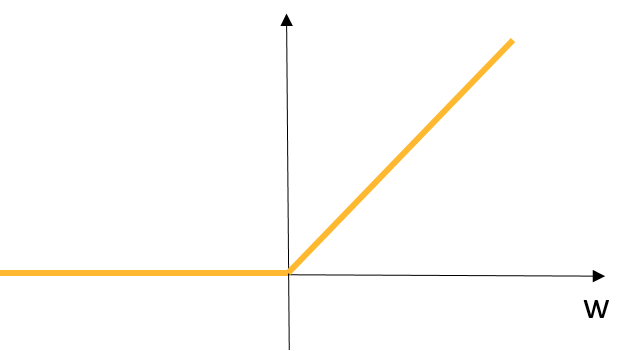
\includegraphics[width=0.32\linewidth]{Dissertation/images/ch1/bayesian_classifier_approximation/relu.png}}
        \hfill
        \subcaptionbox{LeakyReLU(w) = \(max(0.01w, w)\)}{%
            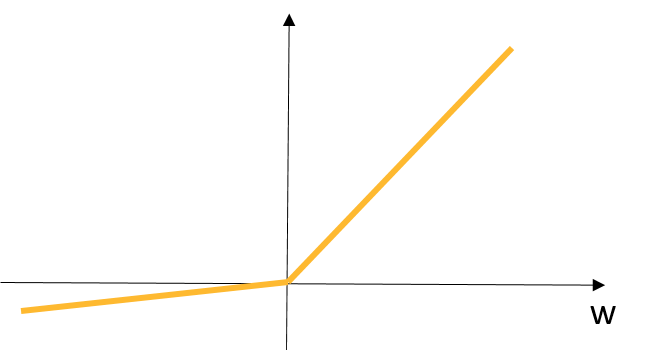
\includegraphics[width=0.32\linewidth]{Dissertation/images/ch1/bayesian_classifier_approximation/leaky_relu.png}}
        \hfill
        \subcaptionbox{Abs(w) = \(|w|\)}{%
            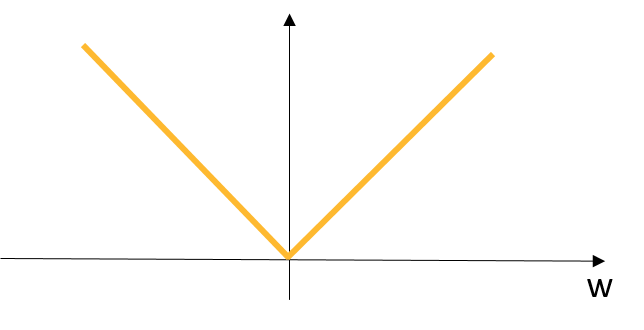
\includegraphics[width=0.32\linewidth]{Dissertation/images/ch1/bayesian_classifier_approximation/abs.png}}
        \hfill
    }
    \caption{Кусочно-линейные функции активации}
    \label{fig:activations}
\end{figure}

Пусть выборка \((X, Y)\) имеет на \(\mathbb{S}\) равномерно непрерывную плотность \(f(X)\):

\[
    f(X) = p_{-1} f_{-1}(X) + p_{+1} f_{+1}(X),
\]

\noindent где \(f_{-1}\) и \(f_{+1}\) -- плотности классов \(-1\) и \(+1\) соответственно.

Для формирования выборки из смеси реальных данных и ``фона`` с плотностью \(\alpha f(X) + (1 - \alpha) p(X)\) добавим к этой выборке искуственно сгенерированные данные \(\{(X_{n+1}, Y_{n+1}), \dots, (X_{2n}, Y_{2n})\}\), где векторы \(\{X_{n+1}, \dots, X_{2n}\}\) -- наблюдения независимо равномерно распределённых на \([0, 1]^d\) случайных векторов c плотностью \(p(X)\), а \(Y_{n+i} = 0, i=1..n\).

Пусть \(C(L, k)\) -- множество всех многослойных персептронов \(c(X)\) с одним нейроном с линейной функцией активации в выходном слое, кусочно-линейной функцией активации \(|\cdot|\) (модульная) в скрытых слоях и числом \(L\) и размером \(k\) скрытых слоёв.

\nomenclature{\(C(L, k)\)}{множество всех многослойных персептронов \(c(X)\) с одним нейроном с линейной функцией активации в выходном слое, кусочно-линейной функцией активации \(|\cdot|\) в скрытых слоях и числом \(L\) и размером \(k\) скрытых слоёв}

Применяя некоторый алгоритм оптимизации (градиентный спуск~\cite{amari1993backpropagation}, генетический алгоритм~\cite{seiffert2001multiple} и т.д.), построим выборочную оценку решения задачи~\cref{eq:regression_approx}:

\begin{equation}
    \label{eq:perceptron_optimization}
    \sum\limits_{i=1}^{2n} (c_n(X_i) - Y_i)^2 \rightarrow \min\limits_{c_n(X)\in C(L, k)},
\end{equation}

\noindent где параметры \(L\) и \(k\) выбраны оптимально с учётом ограничений, связанных с переобучением.

Пусть функция \(c_n^*(X)\) -- решение оптимизационной задачи~\cref{eq:perceptron_optimization}, которая в дальнейшем будет называться \textbf{функцией нейросетевой регрессии}. Соответствующий этому решению персептрон строит иерархическое (по слоям) разбиение компакта \([0, 1]^d\) на \(O(k^{dL})\) непересекающихся ячеек~\cite{devroye2013probabilistic} (при \(k > d\)).

\nomenclature{\(c_n^*(X)\)}{функция нейросетевой регрессии}

\begin{figure}[ht]
    \centerfloat{
        \hfill
        \subcaptionbox{Ячейки первого слоя: 18}{%
            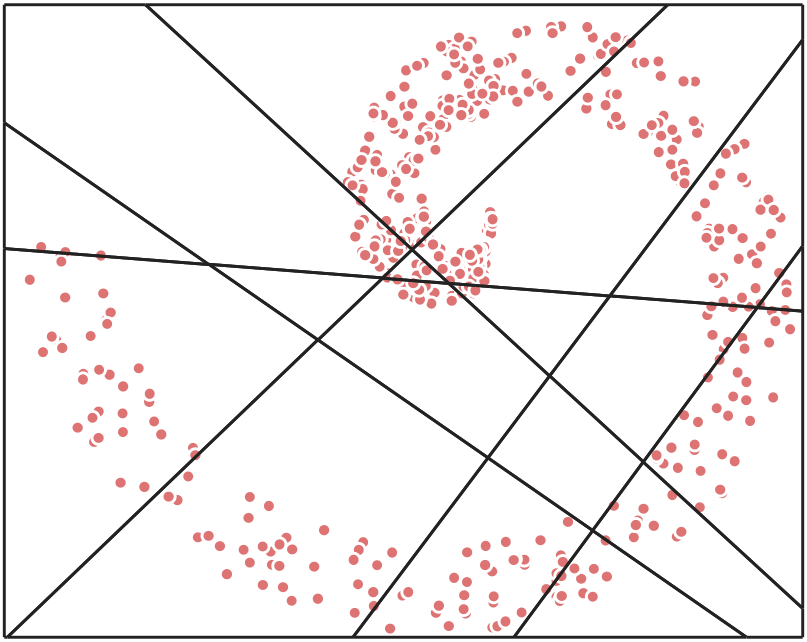
\includegraphics[width=0.3\linewidth]{Dissertation/images/ch1/bayesian_classifier_approximation/partition_l1.png}}
        \hfill
        \subcaptionbox{Ячейки второго слоя: 121}{%
            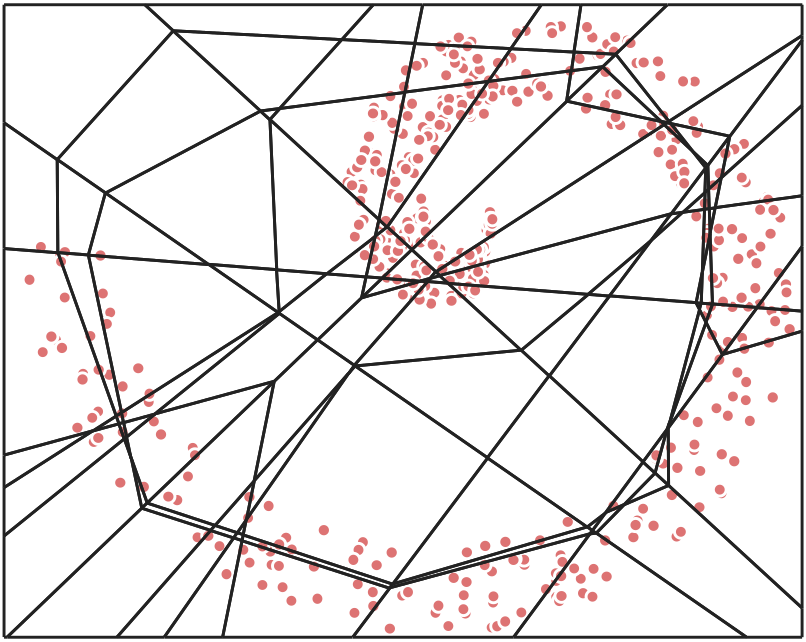
\includegraphics[width=0.3\linewidth]{Dissertation/images/ch1/bayesian_classifier_approximation/partition_l2.png}}
        \hfill
        \subcaptionbox{Ячейки выходного слоя: 148}{%
            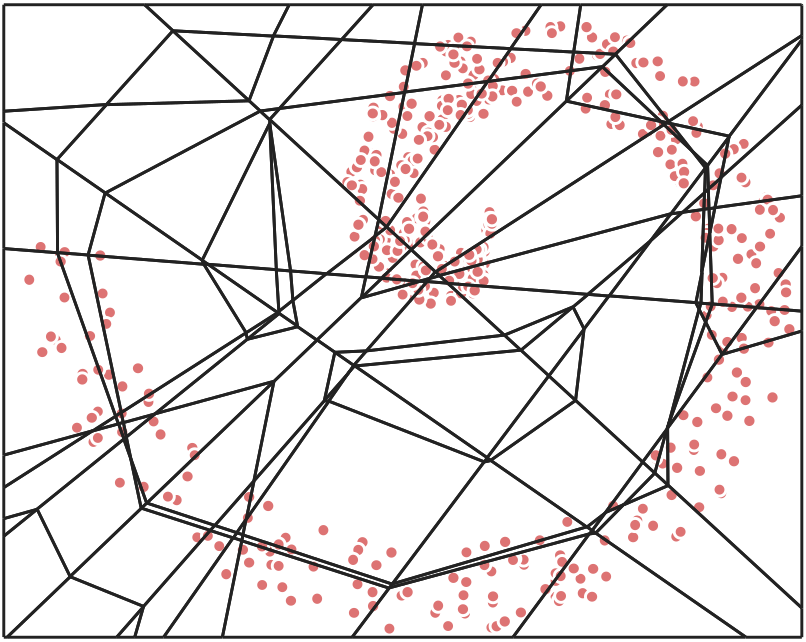
\includegraphics[width=0.3\linewidth]{Dissertation/images/ch1/bayesian_classifier_approximation/partition_l3.png}}
        \hfill
    }
    \caption{Пример разбиения некоторым персептроном с \(L=2\), \(k=6\)}
    \label{fig:perceptron_partition}
\end{figure}

Пример такого разбиения показан на рисунке~\cref{fig:perceptron_partition}, где персептрон имеет \(L=2\) скрытых слоя по \(k=6\) нейронов.

%%%%%%%%%%%%%%%%%%%%%%%%%%%%%%%%%%%%%%%%%%%%%%%%%%%%%%%%%%%%%%%%%%%%%%%%%%%%%%%%%%%%%%%%%%%%%%%%%%%%%%%%%%%%%%%
\subsection{Адаптивная гистограммная аппроксимация}\label{subsec:ch1/histogram_approximation}

Пусть в результате построения \(c_n^*(X)\) получено разбиение компакта \([0, 1]^d\) на \(N\) непересекающихся ячеек \(\{K_1, K_2, \dots, K_N\}\). Рассмотрим кусочно-постоянную (в общем случае разрывную) \textbf{функцию гистограммной регрессии} \(h_n(X)\), принимающую постоянные значения в ячейках разбиения \([0, 1]^d\) и решим для неё оптимизационную задачу:

\nomenclature{\(h_n^*(X)\)}{функция гистограммной регрессии}

\begin{equation}
    \label{eq:histogram_optimization}
    \sum\limits_{i=1}^{2n} (h_n(X_i) - Y_i)^2 \rightarrow \min\limits_{h_n(X)},
\end{equation}

Пусть \(X \in K_r\). Тогда задачу~\cref{eq:histogram_optimization} для этой ячейки можно представить в следующем виде:

\nomenclature{\(K_r\)}{некоторая ячейка из разбиения компакта \([0,1]^d\)}

\begin{equation}
    \label{eq:histogram_cell_optimization}
    n_{-1}(X)\cdot(h_n(X) + 1)^2 + n_0(X)\cdot(h_n(X) - 0)^2 + n_{+1}(X)\cdot(h_n(X) - 1)^2 \rightarrow \min\limits_{h_n(X)},
\end{equation}

\noindent где \(n_j = \sum\limits_{i=1}^{2n} I_{X_i \in K_r, Y_i = j}\).

После дифференцирования функции~\cref{eq:histogram_cell_optimization} по \(h_n(X)\) получаем решение задачи~\cref{eq:histogram_optimization}:

\begin{equation}
    \label{eq:histogram_cell_solution}
    h_n^*(X) = \frac{n_{+1}(X) - n_{-1}(X)}{n_{-1}(X) + n_0(X) + n_{+1}(X)}.
\end{equation}

Пример вычисления функции гистограммной регрессии показан на рисунке~\cref{fig:histogram_evaluation}.

\fixme{ЗАМЕНИТЬ РИСУНОК}
\begin{figure}[ht]
    \centerfloat{
        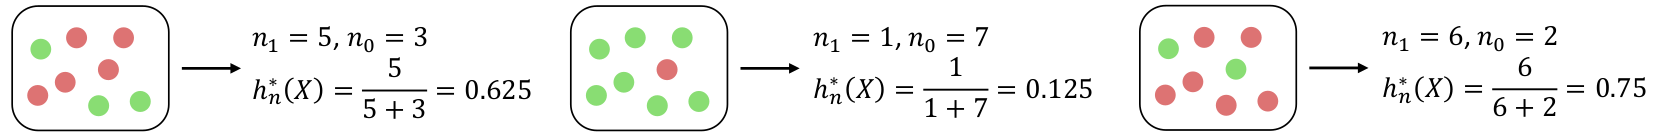
\includegraphics[width=\linewidth]{Dissertation/images/ch1/bayesian_classifier_approximation/histogram_evaluation.png}
    }
    \caption{Пример вычисления \(h_n^*(X)\) в некоторой ячейке \(K_r\)}
    \label{fig:histogram_evaluation}
\end{figure}

Основными достоинствами использования такой аппроксимации являются независимость от масштаба и отсутствие необходимости введения метрик, как того требуют методы на основе расстояний вроде \(k\) ближайших соседей.
\section{Объясняющее двоичное дерево eXBTree}\label{sec:ch1/exbtree}

%%%%%%%%%%%%%%%%%%%%%%%%%%%%%%%%%%%%%%%%%%%%%%%%%%%%%%%%%%%%%%%%%%%%%%%%%%%%%%%%%%%%%%%%%%%%%%%%%%%%%%%%%%%%%%%
\subsection{Построение объясняющего дерева решений}

Как было сказано в разделе~\cref{subsec:ch1/neural_approximation}, многослойный персептрон с кусочно-линейной функцией активации разбивает входное пространство признаков на \(N\) непересекающихся ячеек \(\{K_1, K_2, \ldots, K_N\}\). В каждой такой ячейке значение выходного нейрона определяется фиксированной линейной комбинацией признаков.

Рассмотрим полносвязный персептрон с \(L\) скрытыми слоями по \(k\) нейронов в каждом. В качестве функции активации используется модуль: 
\[
\sigma(z) = |z|.
\]

Обозначим выходы нейронов первого скрытого слоя через \(A_i\), второго -- через \(B_i\), третьего -- через \(C_i\), и так далее (рисунок~\cref{fig:perceptron_architecture}). Для произвольного нейрона слоя \(A\) выполняется:
\[
A_i = \left| \sum_{j=1}^{d} a_{ij} x_j + a_{i0} \right|,
\]
где \( x \in [0, 1]^d \) -- входной вектор признаков. Аналогично, для следующего слоя:
\[
B_i = \left| \sum_{j=1}^{k} b_{ij} A_j + b_{i0} \right|,
\]
и так далее до выходного слоя:
\[
    c_n(x) = \sum_{j=1}^{k} c_{j} B_j + c_{0}.
\]

\begin{figure}[ht]
    \centerfloat{
        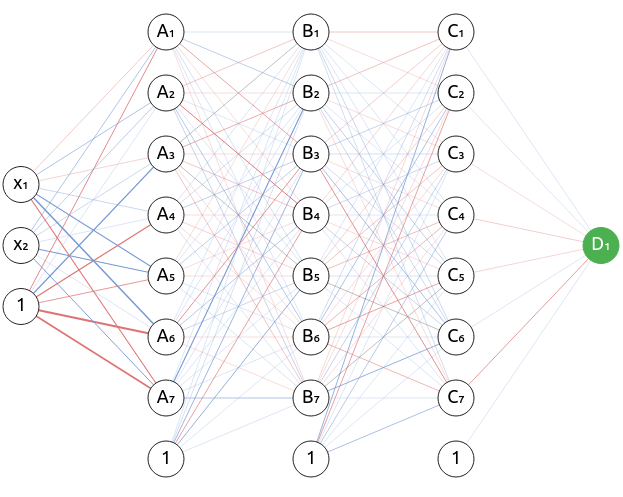
\includegraphics[width=\linewidth]{Dissertation/images/ch1/exbtree/perceptron.png}
    }
    \caption{Архитектура многослойного персептрона с \(d=2\), \(L=3\), \(k=7\)}
    \label{fig:perceptron_architecture}
\end{figure}

Каждый нейрон разбивает своё входное пространство на две области: одну, в которой входная сумма положительна (в этом случае модуль раскрывается со знаком «плюс»), и другую, где сумма отрицательна (в этом случае модуль раскрывается со знаком «минус»). Таким образом, на каждом шаге можно заменить модуль линейным выражением с соответствующим знаком.

Пошагово раскрывая модули в нейронах первого слоя, можно сформировать дерево, в котором каждый путь соответствует определённой комбинации знаков раскрытия модулей. В узлах дерева находятся неравенства, задаваемые условиями перехода: при переходе по левой ветви знак раскрытия модуля в текущем нейроне отрицателен, по правой -- положителен. После обработки всех нейронов слоя \(A\) все функции активации будут раскрыты, и входы к следующему слою \(B\) становятся кусочно-линейными выражениями, зависящими от исходных переменных \(x_j\), и процесс повторяется.

Таким образом, можно построить объясняющее двоичное дерево решений~\cite{song2015decision}, в дальнейшем называемое \textbf{eXBTree} (eXplanatory Binary Tree), в котором каждая вершина соответствует разбиению пространства по линейному неравенству одного нейрона, а каждая листовая вершина -- конечной линейной функции выходного слоя, полученной на конкретной ячейке пространства. Последовательность знаков, с которыми раскрывались активационные функции нейронов по пути от входа к выходному нейрону кодирует произвольную ветку в построенном дереве (рисунок~\cref{fig:exbtree_example}).

\nomenclature{eXBTree}{двоичное дерево решений, построенное на основе многослойного персептрона}

\begin{figure}[ht]
    \centerfloat{
        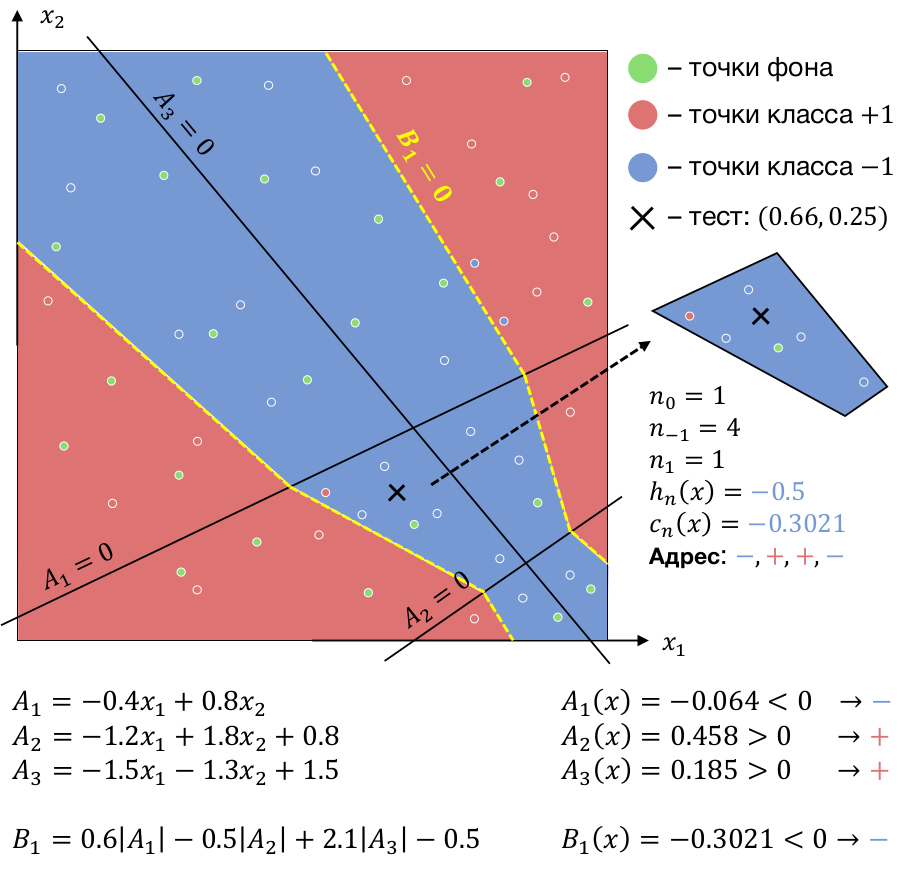
\includegraphics[width=\linewidth]{Dissertation/images/ch1/exbtree/exbtree.png}
    }
    \caption{Пример eXBTree на основе персептрона с \(d = 2\), \(L = 1\), \(k = 3\)}
    \label{fig:exbtree_example}
\end{figure}

Наличие такой структуры позволяет не только интерпретировать классификацию конкретного наблюдения (путь через дерево), но и формировать иерархию разбиений пространства, объединяя соседние ветви дерева на разных уровнях. Это открывает возможности для оценки доверия и анализа прецедентов -- как в пределах отдельной ячейки, так и на объединённых областях пространства.

%%%%%%%%%%%%%%%%%%%%%%%%%%%%%%%%%%%%%%%%%%%%%%%%%%%%%%%%%%%%%%%%%%%%%%%%%%%%%%%%%%%%%%%%%%%%%%%%%%%%%%%%%%%%%%%
\subsection{Комбинаторная сложность и практическая реализация eXBTree}

\begin{theorem}[О сложности построения дерева по многослойному персепртону]
    Пусть многослойный персептрон состоит из \(L\) скрытых слоёв по \(k\) нейронов в каждом (\(k > d\), где \(d\) -- размерность входного пространства). Тогда временная сложность построения двоичного дерева решений по персептрону составляет \(\mathcal{O}(k^{dL})\).
\end{theorem}
\fixme{ДОКАЗАТЕЛЬСТВО}

Тем не менее, в рамках задач классификации или аппроксимации нас интересуют не все возможные ячейки, а лишь те, в которые попали обучающие (или тестовые) наблюдения. Таким образом, нет необходимости в полном построении дерева. Достаточно определить множество фактически реализованных путей, то есть таких комбинаций знаков при раскрытии модулей, которые соответствуют реально встречающимся входным точкам.

Это приводит к следующему практическому алгоритму: каждое наблюдение при прямом проходе через сеть порождает набор знаков уравнений нейронов (до применения активационной функции), который можно трактовать как адрес ячейки. Хранить необходимо лишь такие уникальные адреса, тем самым получая компактное и эффективное представление разбиения пространства, ограниченное данными.

\begin{theorem}[О временной сложности получения решения по построенному дереву]
    Временная сложность получения ответа по построенному дереву решения совпадает со сложностью применения многослойного персептрона и составляет \(\mathcal{O}(kd + Lk^2)\).
\end{theorem}
\fixme{ДОКАЗАТЕЛЬСТВО}

%%%%%%%%%%%%%%%%%%%%%%%%%%%%%%%%%%%%%%%%%%%%%%%%%%%%%%%%%%%%%%%%%%%%%%%%%%%%%%%%%%%%%%%%%%%%%%%%%%%%%%%%%%%%%%%
\subsection{Геометрический анализ построенного дерева}

Рассмотрим свойства дерева, построенного на основе модифицированного обучающего множества с фоновыми наблюдениями, описанного ранее. В каждом внутреннем узле такого дерева содержится линейное неравенство, возникающее из перехода через гиперплоскость активации некоторого нейрона персептрона \(c_n^*(X)\). Каждая вершина дерева соответствует определённой комбинации знаков выражений вида~\(a_i^\top x + a_0\) и, следовательно, описывает подмножество признакового пространства -- выпуклый многогранник, ограниченный системой линейных неравенств.

В каждом листе дерева подсчитывается число объектов обучающего множества, попавших в соответствующую ячейку, с разбиением по классам: \(n_{-1}\), \(n_0\) и \(n_{+1}\). Таким образом, каждый лист фактически содержит гистограмму классов, обсуждавшуюся в разделе~\cref{subsec:ch1/histogram_approximation}. Эти гистограммы позволяют оценивать апостериорные вероятности классов в пределах каждой ячейки и выявлять области с высокой или низкой степенью уверенности модели.

Полученное дерево может быть также рассмотрено как дерево решений с линейными функциями разделения в узлах~\cite{devyatkinpostroenie}, в отличие от традиционных деревьев, в которых узлы соответствуют пороговым условиям вида \(x_j < c\). Такое представление делает поведение многослойного персептрона интерпретируемым: каждый путь от корня до листа соответствует системе линейных неравенств, описывающих область пространства, где модель принимает определённое решение линейным образом.

Важно подчеркнуть, что данная структура обеспечивает интерпретируемость модели в геометрических терминах, что традиционно считается слабой стороной нейронных сетей~\cite{salih2024linear}. В частности, можно явно указать, при каких линейных соотношениях между признаками модель принимает то или иное решение, и каков уровень уверенности классификатора в пределах каждой ячейки. Это позволяет использовать построенное дерево не только как аппроксиматор функции принятия решений, но и как инструмент визуального и количественного анализа поведения модели в различных областях признакового пространства.

%%%%%%%%%%%%%%%%%%%%%%%%%%%%%%%%%%%%%%%%%%%%%%%%%%%%%%%%%%%%%%%%%%%%%%%%%%%%%%%%%%%%%%%%%%%%%%%%%%%%%%%%%%%%%%%
\subsection{Анализ прецедентов и локальной уверенности}

Для повышения интерпретируемости построенного дерева и повышения доверия пользователя к решению важным является анализ конкретных прецедентов -- обучающих объектов, попавших в ту же ячейку дерева, что и тестируемое наблюдение. Вместо представления лишь числового выхода модели (например, вероятности класса 0.98), полезно показать близкие по признаковому пространству точки из обучающей выборки, что даёт наглядное представление о локальном окружении и структуре данных. Таким образом, построенное дерево служит своеобразной псевдо-метрикой, определяющей локальную близость объектов на основе разбиения пространства признаков.

Каждый лист дерева соответствует области признакового пространства, ограниченной системой линейных неравенств. В пределах этой области подсчитывается статистика по объектам различных классов. Однако в реальных задачах, особенно в медицинских и других высокорисковых прикладных областях, объёмы доступных данных могут быть недостаточными для надёжной статистической оценки на уровне отдельных ячеек.

В таких случаях целесообразно рассматривать информацию о соседних ячейках того же уровня дерева. Соседями называются ячейки, отличающиеся значением только одного из предикатов на пути от корня. Если в рассматриваемой ячейке содержится недостаточное количество наблюдений (например, менее заданного порога \(n_\text{min}\)), то можно агрегировать информацию с её соседями для получения более устойчивой оценки локального распределения классов.

Альтернативным подходом является подъём на уровень выше по дереву, то есть укрупнение ячейки за счёт устранения одного из условий, ограничивающих пространство. Это приводит к рассмотрению более широкой области признакового пространства, в которой ожидается большее количество обучающих объектов. Полученная таким образом укрупнённая ячейка также может быть проанализирована с точки зрения гистограммы классов, как описано выше, обеспечивая оценку апостериорной вероятности при недостаточной локальной уверенности.

Подобная стратегия, основанная на анализе прецедентов, позволяет реализовать согласованную схему оценки доверия к решению модели: в случае низкой уверенности по статистике на текущем уровне происходит адаптивное укрупнение области анализа. Это даёт практический механизм для отказа от принятия решения в условиях недостаточной информации и одновременно повышает надёжность выводов, что особенно важно в высокорисковых прикладных задачах.

\section{Связь нейросетевой и гистограммной аппроксимаций. Асимптотические свойства гистограммной аппроксимации}\label{sec:ch1/hist_neural_approximations}

Гистограммная аппроксимация, как было показано выше, представляет собой естественный способ приближённой оценки апостериорной вероятности класса по обучающим данным. В каждой ячейке пространства признаков, определённой системой линейных неравенств, оценивается эмпирическое распределение классов на основе количества объектов, попавших в соответствующую область. В частности, выход функции гистограммной аппроксимации можно записать как

\[
h_n^*(X) = \frac{n_{+1}(X) - n_{-1}(X)}{n_{-1}(X) + n_0(X) + n_{+1}(X)},
\]

где \(n_{-1}(X)\) и \(n_{+1}(x)\) -- количество объектов классов \(-1\) и \(+1\) соответственно, а \(n_0\) -- количество фоновых точек в ячейке, содержащей наблюдение \(X\).

Таким образом, \(h_n^*(X)\) соответствует разности логарифмов аппроксимированных правдоподобий классов и служит приближением разности апостериорных вероятностей.

Предполагая, что плотности распределения классов равномерно непрерывны, можно показать, что гистограмма является строго состоятельной оценкой этих плотностей. Результаты работы~\cite{devroye2013probabilistic} позволяют утверждать, что при росте объёма обучающей выборки \(n \to \infty\) и одновременном увеличении числа ячеек (или, эквивалентно числа нейронов \(kL \to \infty\), отвечающего за глубину разбиения пространства) имеет место следующее соотношение:

\begin{equation}
    \label{eq:binary_consistency}
    \mathbb{E}\left( h_n^*(X) - c_n^*(X) \right)^2 \to 0, \quad n \to \infty,    
\end{equation}

где \(c_n^*(x)\) -- выход модифицированного персептрона, аппроксимирующего байесовскую границу принятия решения.

Этот результат обосновывает возможность замены гистограммной аппроксимации на нейросетевую, сохраняющую асимптотические свойства при существенно меньших требованиях к вычислительным ресурсам. В отличие от гистограммы, для работы персептрона не требуется хранение всей обучающей выборки или экспоненциально большого числа ячеек.

Следствием приведённого утверждения является практический критерий принятия решения на основе выхода персептрона. Поскольку \(c_n^*(x)\) приближает \(h_n^*(x)\), то в условиях асимптотической сходимости разумно вводить порог отказа \(\beta\) и принимать решение о принадлежности к одному из классов только при условии

\[
|c_n^*(x)| > \beta.
\]

Тем самым достигается контроль над уверенностью классификатора: чем ближе значение \(c_n^*(x)\) к нулю, тем ниже надёжность предсказания. Предложенная схема позволяет реализовать отказ от ответа в ситуациях, когда классификатор не обладает достаточной апостериорной уверенностью, и одновременно существенно снижает вычислительную сложность по сравнению с прямой реализацией гистограммной аппроксимации.

\section{Случай нескольких классов}\label{sec:ch1/multiclass_case}

Рассмотренные ранее методы касаются задачи бинарной классификации, когда множество допустимых меток ограничено двумя классами. Однако на практике часто возникает необходимость классификации объектов в более чем два класс~\cite{aly2005survey}. Переход от бинарной к многоклассовой классификации существенно усложняет как построение, так и интерпретацию модели~\cite{lorena2008review}.

Существуют два стандартных подхода к решению многоклассовой задачи на основе бинарных классификаторов: стратегия \textbf{один против всех} (one-vs-rest) и стратегия \textbf{попарной классификации} (one-vs-one). В первом случае для каждого из \(C\) классов обучается отдельный бинарный классификатор, который отделяет данный класс от объединения всех остальных. Во втором случае для каждой из \(\frac{C(C-1)}{2}\) пар классов строится бинарный классификатор, различающий только эти два класса, а итоговое решение принимается, например, по большинству голосов или с использованием процедуры агрегации~\cite{galar2011overview}.

Обе стратегии имеют как теоретические, так и практические недостатки. В стратегии один против всех возникает проблема перекоса, связанная с несбалансированностью классов. При наличии сильно преобладающего класса классификаторы могут склоняться к частому отнесению объекта к этому классу, даже если признаки ближе к другому. Это приводит к смещению аппроксимации и, как следствие, к снижению обоснованности принятого решения. Дополнительные методы борьбы с дисбалансом, такие как дублирование редких классов или уменьшение выборки преобладающих, искажают исходное распределение данных, что затрудняет интерпретацию результатов и может приводить к потере статистической достоверности.

Стратегия попарных классификаторов, напротив, требует построения большого числа моделей, число которых растёт квадратично с числом классов. Кроме того, процедура выбора итогового класса по результатам попарных голосований может быть неоднозначной~\cite{kang2015constructing}: возможны случаи, при которых отсутствует чёткий победитель. При этом каждая отдельная модель опирается на подмножество данных, и совокупный результат может не учитывать общую структуру пространства признаков. В результате возникает риск потери согласованности между частными классификаторами, что негативно сказывается на устойчивости системы в целом.

Таким образом, обобщение бинарной модели на многоклассовую постановку сталкивается с рядом фундаментальных затруднений. Проблемы интерпретируемости, статистической состоятельности и устойчивости принятия решений становятся особенно острыми при наличии несбалансированных классов и сложной структуры признакового пространства. Эти соображения подводят к необходимости переосмысления самой постановки задачи классификации, особенно в ситуациях, когда интерес представляет лишь один или малое число целевых классов, а остальные данные играют вспомогательную роль.

\section{Простая линейная атака на персептрон}\label{sec:ch1/slap}

Несмотря на широкую практическую применимость нейросетевых моделей, включая многослойный персептрон, их надёжность может быть существенно снижена при воздействии целенаправленных возмущений, известных как состязательные атаки. Эти атаки используют особенности разделяющей поверхности модели для генерации входных данных, вызывающих ошибочную классификацию. В рамках настоящей работы предложен новый подход к формированию таких примеров, получивший название ``простая линейная атака на персептрон`` (SLAP, Simple Linear Attack for Perceptron). Подробности методики опубликованы в авторской статье~\cite{perminov2024slap}.

\nomenclature{MLP}{многослойный персептрон}

%%%%%%%%%%%%%%%%%%%%%%%%%%%%%%%%%%%%%%%%%%%%%%%%%%%%%%%%%%%%%%%%%%%%%%%%%%%%%%%%%%%%%%%%%%%%%%%%%%%%%%%%%%%%%%%
\subsection{Существующие подходы}

Наиболее распространённые методы формирования атакующих примеров основываются на градиентной оптимизации. В частности, метод FGSM (Fast Gradient Sign Method)~\cite{goodfellow2014explaining} и метод проецированного градиентного спуска PGD (Projected Gradient Descent)~\cite{madry2017towards} находят направления в пространстве входных признаков, по которым можно максимизировать ошибку классификатора. Однако такие подходы требуют итеративных вычислений и чувствительны к выбору гиперпараметров.

Альтернативой являются методы, использующие выпуклую оптимизацию или линейное программирование, например,~\cite{croce2019sparse, wong2018provable}. В настоящей работе предложен подход, основанный исключительно на методах линейной алгебры, позволяющий строить атакующие примеры за счёт решения систем линейных уравнений или неравенств. Подход ориентирован прежде всего на персептроны с кусочно-линейными функциями активации, такими как ReLU, Leaky ReLU и Abs, что позволяет упростить структуру модели до линейных преобразований при фиксированных знаках активации.

%%%%%%%%%%%%%%%%%%%%%%%%%%%%%%%%%%%%%%%%%%%%%%%%%%%%%%%%%%%%%%%%%%%%%%%%%%%%%%%%%%%%%%%%%%%%%%%%%%%%%%%%%%%%%%%
\subsection{Постановка задачи атаки}

\fixme{ЗАМЕНИТЬ \(n\) НА \(d\) и \(m\) на \(C\) поправить рисунки}

Пусть имеется обученный персептрон \(c(x)\), принимающий на вход вектор \(x \in \mathbb{R}^d\) и возвращающий вектор выходных значений \(y \in \mathbb{R}^C\), соответствующих \(C\) (\(C < d\)) классам. Обозначим через \(x_t\) целевой пример (рисунок~\cref{fig:attack_task}\subcaptionref{fig:attack_task_x_t}), на который должна быть «перенесена» классификация, и через \(x_a\) -- пример, который подвергается атаке (рисунок~\cref{fig:attack_task}\subcaptionref{fig:attack_task_x_a}). Требуется построить новый вектор \(x\) (рисунок~\cref{fig:attack_task}\subcaptionref{fig:attack_task_x}), близкий к \(x_a\), но классифицируемый так же, как \(x_t\). Формально, задача формулируется как:

\[
\begin{cases}
    \| x - x_a \| \rightarrow \min,\\
    \| x - x_t \| > 0,\\
    c(x) = c(x_t),
\end{cases}
\quad \text{или} \quad
\begin{cases}
    \| x - x_a \| \rightarrow \min,\\
    \| x - x_t \| > 0,\\
    \arg\max c(x) = \arg\max c(x_t).
\end{cases}
\]

\begin{figure}[ht]
    \centerfloat{
        \hfill
        \subcaptionbox{\(x_t\) -- целевой пример\label{fig:attack_task_x_t}}{%
            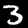
\includegraphics[width=0.3\linewidth]{Dissertation/images/ch1/slap/x_t.png}}
        \hfill
        \subcaptionbox{\(x_a\) -- пример, подвергающийся атаке\label{fig:attack_task_x_a}}{%
            
\includegraphics[width=0.3\linewidth]{Dissertation/images/ch1/slap/x_a.png}}
        \hfill
        \subcaptionbox{\(x\) -- построенный атакующий пример\label{fig:attack_task_x}}{%
            
\includegraphics[width=0.3\linewidth]{Dissertation/images/ch1/slap/x.png}}
        \hfill
    }
    \caption{Примеры, участвующие в атаке на многослойный персептрон}
    \label{fig:attack_task}
\end{figure}

Для повышения скрытности атаки накладываются ограничения на диапазон допустимых значений \(x \in [x_{\min}, x_{\max}]\), где, например, для изображений естественно полагать \(x_{\min} = 0\), \(x_{\max} = 1\).

%%%%%%%%%%%%%%%%%%%%%%%%%%%%%%%%%%%%%%%%%%%%%%%%%%%%%%%%%%%%%%%%%%%%%%%%%%%%%%%%%%%%%%%%%%%%%%%%%%%%%%%%%%%%%%%
\subsection{Атака на однослойный персептрон}

Рассмотрим случай одного слоя, где выходной вектор модели задаётся как \(y = Wx + b\), причём \(W \in \mathbb{R}^{C \times d} \), \(b \in \mathbb{R}^C\).

\subsubsection{Без учёта ограничений на входные значения}

Предположим, что матрицу \(W\) можно разбить на подматрицы \(W_1 \in \mathbb{R}^{C \times C}\) и \(W_2 \in \mathbb{R}^{C \times (d - C)}\), выбрав, например, первые (или случайные для большей незаметности) \(C\) столбцов. Аналогично разбиваем вектор \(x_a\) на \(x_{a_1} \in \mathbb{R}^C\) и \(x_{a_2} \in \mathbb{R}^{d - C}\). Тогда атакующий вектор может быть получен по формуле:

\[
x^* = W_1^{-1} \cdot (b^\top - W_2 x_{a_2}),
\]
а полное решение восстанавливается как конкатенация \(x = [x^*, x_{a_2}]\) (рисунок~\cref{fig:matrix_attack}).

\begin{figure}[ht]
    \centerfloat{
        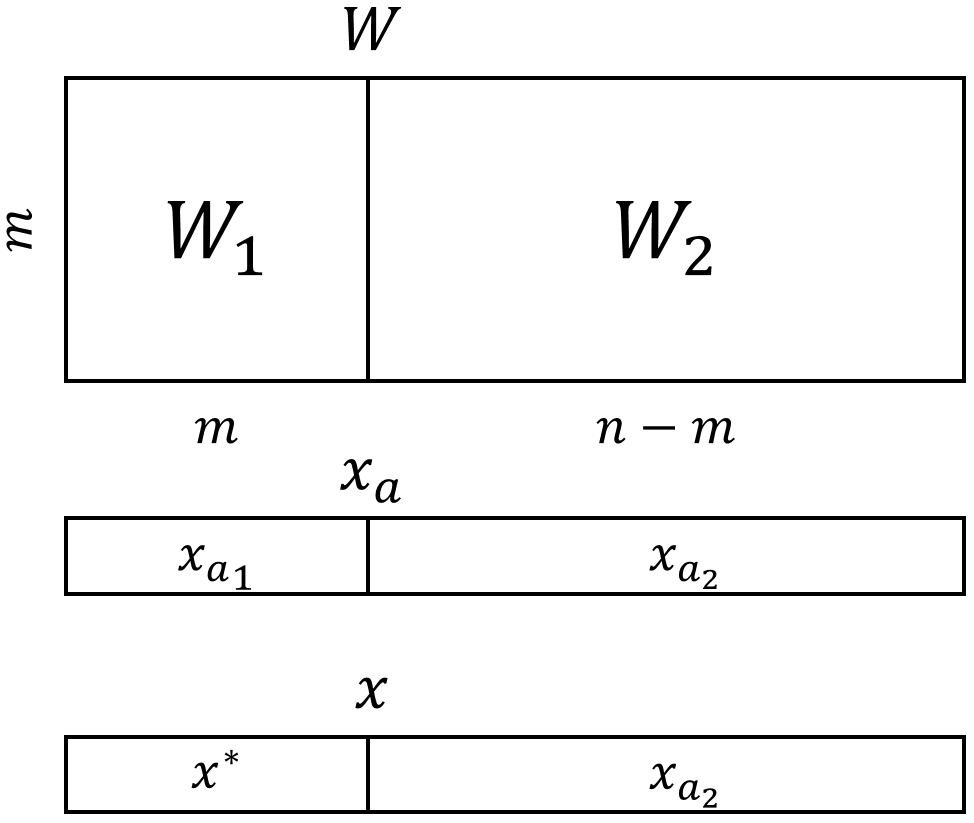
\includegraphics[width=0.7\linewidth]{Dissertation/images/ch1/slap/matrix_attack.png}
    }
    \caption{Схема матричной атаки}
    \label{fig:matrix_attack}
\end{figure}

Данный метод работает исключительно в случае, если матрица \(W_1\) обратима (что почти всегда выполняется при случайной инициализации). Однако он не учитывает допустимые границы значений и чувствителен к квантованию, происходящему при сохранении изображения в файл (рисунок~\cref{fig:matrix_attack_example}).

\begin{figure}[ht]
    \centerfloat{
        \hfill
        \subcaptionbox{\(x_t\) -- целевой пример}{%
            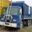
\includegraphics[width=0.3\linewidth]{Dissertation/images/ch1/slap/matrix_x_t.jpeg}}
        \hfill
        \subcaptionbox{\(x_a\) -- пример, который подвергается атаке}{%
            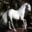
\includegraphics[width=0.3\linewidth]{Dissertation/images/ch1/slap/matrix_x_a.jpeg}}
        \hfill
        \subcaptionbox{\(x\) -- построенный атакующий пример}{%
            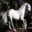
\includegraphics[width=0.3\linewidth]{Dissertation/images/ch1/slap/matrix_x.jpeg}}
        \hfill
    }
    \caption{Пример матричной атаки, \(x \in [-1055, 926]\)}
    \label{fig:matrix_attack_example}
\end{figure}

\subsubsection{С учётом ограничений}

Более реалистичный подход включает в себя формулировку задачи как квадратичной оптимизации:

\[
\begin{cases}
    \frac{1}{2} x^\top P x + q^\top x \rightarrow \min,\\
    Ax = b,\\
    x_{\min} \leq x \leq x_{\max},
\end{cases}
\]
где в простейшем случае \(P = E\) -- единичная матрица, \(q = -x_a\), \(A = W\), \(b = y_t - b\). Тогда задача принимает вид:

\[
\begin{cases}
    \frac{1}{2} x^\top x + x_a^\top x \rightarrow \min,\\
    Wx = y_t - b,\\
    x \in [x_{\min}, x_{\max}].
\end{cases}
\]

При невозможности точного воспроизведения \(y_t\) возможно ослабление условий за счёт введения допусков \(\epsilon\):

\[
y_t - \epsilon \leq Wx + b \leq y_t + \varepsilon.
\]

Эти неравенства легко переписываются в канонической форме для QP-решателей. Пример применения данного вида атаки приведён на рисунке~\cref{fig:qp_attack_example}.

\begin{figure}[ht]
    \centerfloat{
        \hfill
        \subcaptionbox{\(x_t\) -- целевой пример}{%
            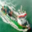
\includegraphics[width=0.3\linewidth]{Dissertation/images/ch1/slap/qp_x_t.png}}
        \hfill
        \subcaptionbox{\(x_a\) -- пример, который подвергается атаке}{%
            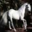
\includegraphics[width=0.3\linewidth]{Dissertation/images/ch1/slap/qp_x_a.png}}
        \hfill
        \subcaptionbox{\(x\) -- построенный атакующий пример}{%
            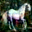
\includegraphics[width=0.3\linewidth]{Dissertation/images/ch1/slap/qp_x.png}}
        \hfill
    }
    \caption{Пример QP атаки}
    \label{fig:qp_attack_example}
\end{figure}

%%%%%%%%%%%%%%%%%%%%%%%%%%%%%%%%%%%%%%%%%%%%%%%%%%%%%%%%%%%%%%%%%%%%%%%%%%%%%%%%%%%%%%%%%%%%%%%%%%%%%%%%%%%%%%%
\subsection{Атака на многослойный персептрон}

При наличии нескольких слоёв в сети возникает проблема нелинейности из-за активационных функций. Однако, если эти функции кусочно-линейны (ReLU, Leaky ReLU, Abs), то при фиксированных знаках аргументов они представляют собой линейные отображения. Например, функция ReLU ведёт себя как \(x\) при \(x \geq 0\) и как \(0\) при \(x < 0\).

Рассмотрим модель из трёх слоёв:

\[
y = W_3 \cdot f_2(W_2 \cdot f_1(W_1 x + b_1) + b_2) + b_3.
\]

Предположим, что знаки активации известны (например, получены от прямого прохода по \(x_t\)). Тогда последовательное раскрытие слоёв позволяет свести сеть к линейной модели. Например, если все значения после первого слоя положительны (т.е. активация \(f_1\) действует как тождественная функция), а после второго -- отрицательны (и активация действует как умножение на константу), можно получить:

\[
\begin{cases}
    W_1x + b_1 \geq 0\\
    W_2W_1x + W_2b_1 + b_2 \leq 0\\
    y = -(W_3W_2W_1x + W_3W_2b_1 + W_3b_2) + b_3 
\end{cases}
\]
где коэффициенты \(W_{321}\), \(b_{321}\) выражаются через произведения матриц весов и сдвигов. Тогда атака сводится к аналогичной задаче QP, но при дополнительных ограничениях на знаки промежуточных переменных:

\[
\begin{cases}
    W_{21} = W_2W_1\\
    b_{21} = W_2b_1 + b_2\\
    W_{321} = -W_3W_2W_1\\
    b_{321} = b_3 - W_3W_2b_1 - W_3b_2\\
    W_1x + b_1 \geq 0\\
    W_{21}x + b_{21} \leq 0\\
    y = W_{321}x + b_{321}
\end{cases}
\]

Пример атаки на многослойный персептрон представлен на рисунке~\cref{fig:multilayer_attack_example}.

\begin{figure}[ht]
    \centerfloat{
        \hfill
        \subcaptionbox{\(x_t\) -- целевой пример}{%
            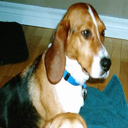
\includegraphics[width=0.3\linewidth]{Dissertation/images/ch1/slap/multilayer_x_t.png}}
        \hfill
        \subcaptionbox{\(x_a\) -- пример, который подвергается атаке}{%
            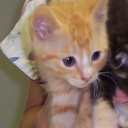
\includegraphics[width=0.3\linewidth]{Dissertation/images/ch1/slap/multilayer_x_a.png}}
        \hfill
        \subcaptionbox{\(x\) -- построенный атакующий пример}{%
            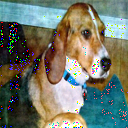
\includegraphics[width=0.3\linewidth]{Dissertation/images/ch1/slap/multilayer_x.png}}
        \hfill
    }
    \caption{Пример атаки на многослойный персептрон на датасете Cat-vs-Dog~\cite{parkhi2012cats}}
    \label{fig:multilayer_attack_example}
\end{figure}

%%%%%%%%%%%%%%%%%%%%%%%%%%%%%%%%%%%%%%%%%%%%%%%%%%%%%%%%%%%%%%%%%%%%%%%%%%%%%%%%%%%%%%%%%%%%%%%%%%%%%%%%%%%%%%%
\subsection{Генерация произвольных входов с заданным выходом}

Так как размерность входа чаще всего превышает размерность выхода, задача построения входа \(x\), удовлетворяющего \(c(x) = y_t\), имеет бесконечно много решений. В этом случае можно случайным образом зафиксировать некоторые координаты \(x\), оставляя другие свободными, и решать полученную переопределённую систему. Это позволяет формировать обширные множества атакующих примеров, обладающих одинаковым выходом сети.

На рисунке~\cref{fig:bonus_attack} приведены примеры атакующих изображений. В первом столбце расположены целевые изображения, соответствующие заданному выходу модели. Второй столбец содержит атакующие примеры, полученные путём минимального возмущения других исходных изображений с целью приведения их к тому же выходу. Остальные столбцы демонстрируют изображения, сгенерированные методом случайного поиска при условии воспроизведения целевого выхода. Все изображения в пределах одной строки имеют идентичный выходной вектор персептрона, несмотря на различия в визуальном представлении.

\begin{figure}[ht]
    \centerfloat{
        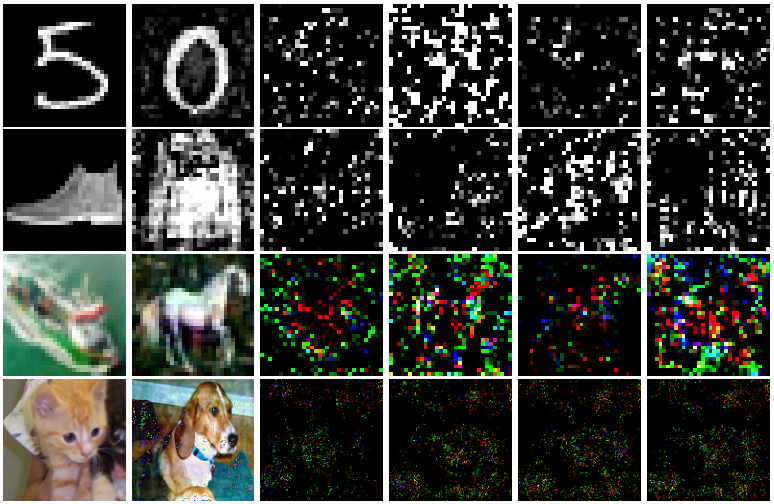
\includegraphics[width=\linewidth]{Dissertation/images/ch1/slap/bonus.png}
    }
    \caption{Пример генерации атакующих примеров}
    \label{fig:bonus_attack}
\end{figure}

%%%%%%%%%%%%%%%%%%%%%%%%%%%%%%%%%%%%%%%%%%%%%%%%%%%%%%%%%%%%%%%%%%%%%%%%%%%%%%%%%%%%%%%%%%%%%%%%%%%%%%%%%%%%%%%
\subsection{Экспериментальное исследование}

Алгоритм был реализован и протестирован на простых персептронах, обученных на датасетах MNIST~\cite{deng2012mnist} и CIFAR-10~\cite{krizhevsky2009learning}. Для каждого изображения из тестовой выборки выбиралось случайное изображение другого класса, и применялась атака, направленная на минимальное изменение первого изображения с целью получения выхода второго. В эксперименте оценивалась \(\ell_\infty\)-норма между оригиналом и атакующим примером. Результаты приведены в таблице~\cref{tab:slap}.

\begin{table} [htbp]
\centering
\begin{threeparttable}
\caption{Результаты применения SLAP атаки}\label{tab:slap}
\begin{SingleSpace}
\begin{tabular}{|l|c|c|c|c|c|c|}
\hline
\multicolumn{1}{|c|}{\multirow{2}{*}{Модель}} &
\multicolumn{1}{|c|}{\multirow{2}{*}{Набор}} &
\multicolumn{1}{|c|}{\multirow{2}{*}{Accuracy}} &
\multicolumn{2}{c|}{Атака на значения} & \multicolumn{2}{c|}{Атака на класс} \\
\cline{4-7}
& & & \(\ell_\infty\) & Accuracy & \(\ell_\infty\) & Accuracy \\
\hline
10               & \multirow{5}{*}{MNIST} & 0.9288 & 0.019 & 0.003 & 0.019 & 0.002 \\
10-10            &                        & 0.9326 & 0.021 & 0.007 & 0.022 & 0.001 \\
100-10           &                        & 0.9805 & 0.052 & 0.009 & 0.051 & 0.005 \\
1000-10          &                        & 0.9849 & 0.091 & 0.012 & 0.092 & 0.009 \\
160-80-40-20-10  &                        & 0.9792 & 0.117 & 0.000 & 0.114 & 0.000 \\
\hline
10               & \multirow{4}{*}{CIFAR10} & 0.3989 & 0.027 & 0.014 & 0.024 & 0.011 \\
100-10           &                          & 0.4853 & 0.054 & 0.032 & 0.055 & 0.018 \\
1000-10          &                          & 0.5236 & 0.095 & 0.041 & 0.096 & 0.023 \\
320-160-80-40-10 &                          & 0.5353 & 0.121 & 0.049 & 0.119 & 0.037 \\
\hline
\end{tabular}
\end{SingleSpace}
\end{threeparttable}
\end{table}

Результаты показывают, что при использовании простых архитектур удаётся достигать атакующих примеров с минимальными отклонениями, зачастую визуально незаметными. При переходе к более глубоким моделям число необходимых изменений возрастает, что объясняется более сложной геометрией границ принятия решений.

%%%%%%%%%%%%%%%%%%%%%%%%%%%%%%%%%%%%%%%%%%%%%%%%%%%%%%%%%%%%%%%%%%%%%%%%%%%%%%%%%%%%%%%%%%%%%%%%%%%%%%%%%%%%%%%
\subsection{Выводы}

Предложенный метод демонстрирует возможность построения состязательных примеров для нейросетевых моделей с кусочно-линейными активациями без использования градиентной информации. Использование методов линейной алгебры позволяет получать как точные, так и приближённые решения с учётом ограничений на значения входных признаков. Атака легко адаптируется к многослойным моделям и может применяться не только к полносвязным сетям, но и к свёрточным архитектурам, обладающим аналогичной линейной структурой.

\section{Применение}\label{sec:ch1/application}

Рассмотренные в предыдущих разделах методы бинарной классификации позволяют успешно решать задачи разделения двух классов на компакте признакового пространства. В данном разделе рассматриваются примеры, иллюстрирующие особенности работы моделей, использующих описанную в разделе~\cref{subsec:ch1/bayesian_classifier_modification} модификацию, а также проблемы, которые такая модификация позволяет эффективно решать.

%%%%%%%%%%%%%%%%%%%%%%%%%%%%%%%%%%%%%%%%%%%%%%%%%%%%%%%%%%%%%%%%%%%%%%%%%%%%%%%%%%%%%%%%%%%%%%%%%%%%%%%%%%%%%%%
\subsection{Поведение вне носителя распределения}

Обычные бинарные классификаторы, обученные по конечной выборке без дополнительного ``фона``, склонны выдавать уверенные предсказания даже в тех точках пространства, где отсутствуют обучающие данные. Это поведение связано с тем, что модель не знает о структуре плотности признаков и минимизирует ошибку лишь на ограниченном множестве точек.

Рассмотрим демонстрационный пример с двумя классами, заданными в виде спиралей на двумерной плоскости. На рисунке~\cref{fig:spirals_example}\subcaptionref{fig:spirals_example_classic} представлено решение, полученное обычным бинарным классификатором. Видно, что модель уверенно относит к одному из классов даже точки, расположенные далеко за пределами области, покрытой обучающими данными.

Для сравнения, если использовать, описанную в разделе~\cref{subsec:ch1/neural_approximation} модифицированную процедуру, то классификатор начинает учитывать общую структуру распределения данных и классифицирует ``внешние`` точки как фон (рисунок~\cref{fig:spirals_example}\subcaptionref{fig:spirals_example_modified}). Это значительно повышает надёжность предсказаний и позволяет говорить о появлении эффекта отказа от распознавания вне носителя распределения.

\begin{figure}[ht]
    \centerfloat{
        \hfill
        \subcaptionbox{классический классификатор\label{fig:spirals_example_classic}}{%
            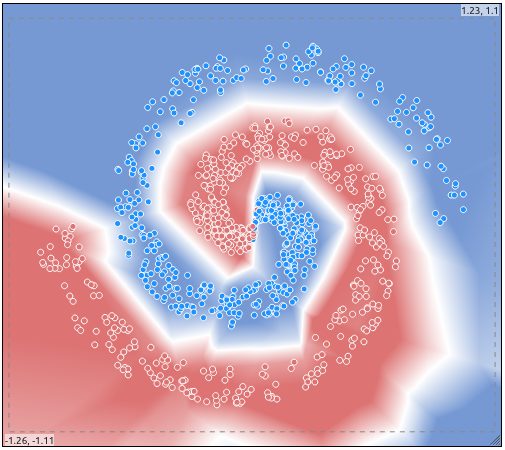
\includegraphics[width=0.48\linewidth]{Dissertation/images/ch1/application/spirals_usual.png}}
        \hfill
        \subcaptionbox{модифицированный классификатор\label{fig:spirals_example_modified}}{%
            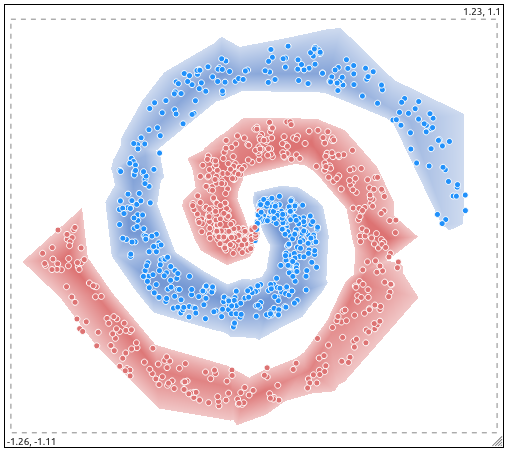
\includegraphics[width=0.48\linewidth]{Dissertation/images/ch1/application/spirals_modified.png}}
        \hfill
    }
    \caption{Сравнение поведения классификаторов вне носителя}
    \label{fig:spirals_example}
\end{figure}

%%%%%%%%%%%%%%%%%%%%%%%%%%%%%%%%%%%%%%%%%%%%%%%%%%%%%%%%%%%%%%%%%%%%%%%%%%%%%%%%%%%%%%%%%%%%%%%%%%%%%%%%%%%%%%%
\subsection{Устойчивость}

Модели, обучаемые без использования фона, оказываются чрезвычайно чувствительными к отдельным аномальным точкам. Добавление даже одной точки может радикально изменить форму решающего правила (рисунок~\cref{fig:backdor_attack}\subcaptionref{fig:backdor_attack_classic}). Это явление лежит в основе так называемых backdoor-атак~\cite{guo2022overview}, когда намеренно добавленные в обучающую выборку точки провоцируют нежелательное поведение модели в заранее заданной области.

Добавление фона значительно снижает эффект подобных атак (рисунок~\cref{fig:backdor_attack}\subcaptionref{fig:backdor_attack_modified}). Чтобы в присутствии фона точка начала влиять на решение, необходимо существенно увеличить её плотность, что требует добавления множества подобных примеров. Таким образом, обучение с фоном повышает устойчивость модели к целевым модификациям данных.

\begin{figure}[ht]
    \centerfloat{
        \hfill
        \subcaptionbox{классический классификатор\label{fig:backdor_attack_classic}}{%
            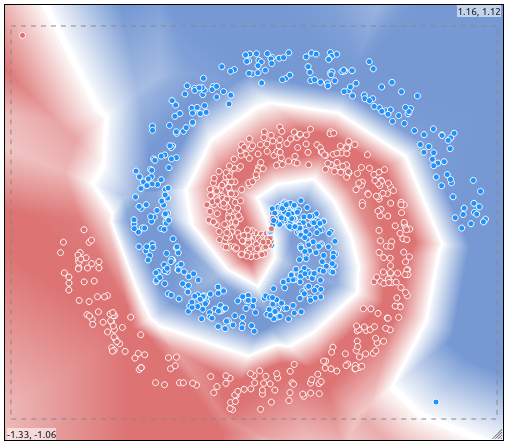
\includegraphics[width=0.48\linewidth]{Dissertation/images/ch1/application/backdor_usual.png}}
        \hfill
        \subcaptionbox{модифицированный классификатор\label{fig:backdor_attack_modified}}{%
            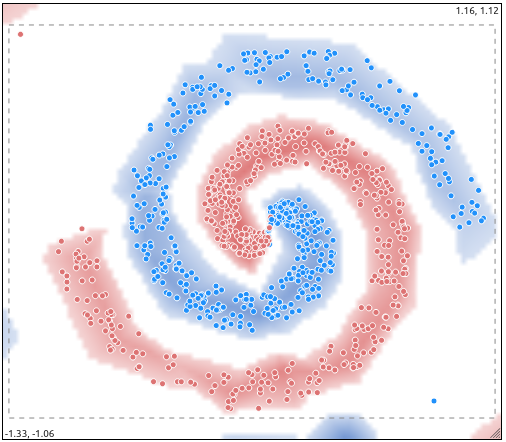
\includegraphics[width=0.48\linewidth]{Dissertation/images/ch1/application/backdor_modified.png}}
        \hfill
    }
    \caption{Сравнение устойчивости классификаторов к backdoor-атаке}
    \label{fig:backdor_attack}
\end{figure}

%%%%%%%%%%%%%%%%%%%%%%%%%%%%%%%%%%%%%%%%%%%%%%%%%%%%%%%%%%%%%%%%%%%%%%%%%%%%%%%%%%%%%%%%%%%%%%%%%%%%%%%%%%%%%%%
\subsection{Противодействие SLAP атаке}

Одним из наиболее уязвимых мест классических классификаторов является их поведение на границе принятия решений. Это свойство активно используется в рамках предложенной в разделе~\cref{sec:ch1/slap} атаки SLAP.

Модифицированная процедура классификации, использующая фоновый класс, существенно снижает эффективность подобного рода атак. На рисунке~\cref{fig:slap_modified_attack} представлены примеры атак, полученных с использованием метода SLAP как для классической модели, так и для модели с фоном. При этом использование модифицированной процедуры обучения приводит к следующим эффектам:

\begin{itemize}
  \item во многих случаях атака не удаётся;
  \item при отсутствии ограничений на допустимую область признаков атакующие точки часто выходят за пределы компакта, что приводит к отказу от их распознаванию;
  \item при успешной атаке полученные точки, как правило, попадают в области с низким уровнем доверия, что также приводит к отказу от распознавания.
\end{itemize}

Таким образом, модификация классификатора с введением фонового класса позволяет эффективно нейтрализовать атаку SLAP, построенную без использования градиентной информации и не зависящую от конкретной архитектуры модели.

%%%%%%%%%%%%%%%%%%%%%%%%%%%%%%%%%%%%%%%%%%%%%%%%%%%%%%%%%%%%%%%%%%%%%%%%%%%%%%%%%%%%%%%%%%%%%%%%%%%%%%%%%%%%%%%
\subsection{Сопоставление нейросетевой и гистограммной регрессии}

В разделе~\cref{subsec:ch1/histogram_approximation} рассматривалось иерархическое разбиение компакта нейросетевой моделью на ячейки, на основе которых строилась функция гистограммной регрессии. Визуальное сопоставление результатов нейросетевой и гистограммной регрессий подтверждает близость этих методов: выход нейросети в силу своей непрерывности плавно переходит от одного класса к другому, приближая собой ступенчатую структуру гистограммы (рисунок~\cref{fig:cn_vs_hn}). Ячейки гистограммы, на которые разбивает пространство персептрон, окрашены в соответствии со значением \(h_n^*(X)\) в ячейке и визуально очень похожи на выход нейросети.

Это наблюдение позволяет рассматривать регрессию на выходе многослойного персептрона как мягкую версию гистограммной аппроксимации, реализуемую при помощи кусочно-линейных функций.

\begin{figure}[ht]
    \centerfloat{
        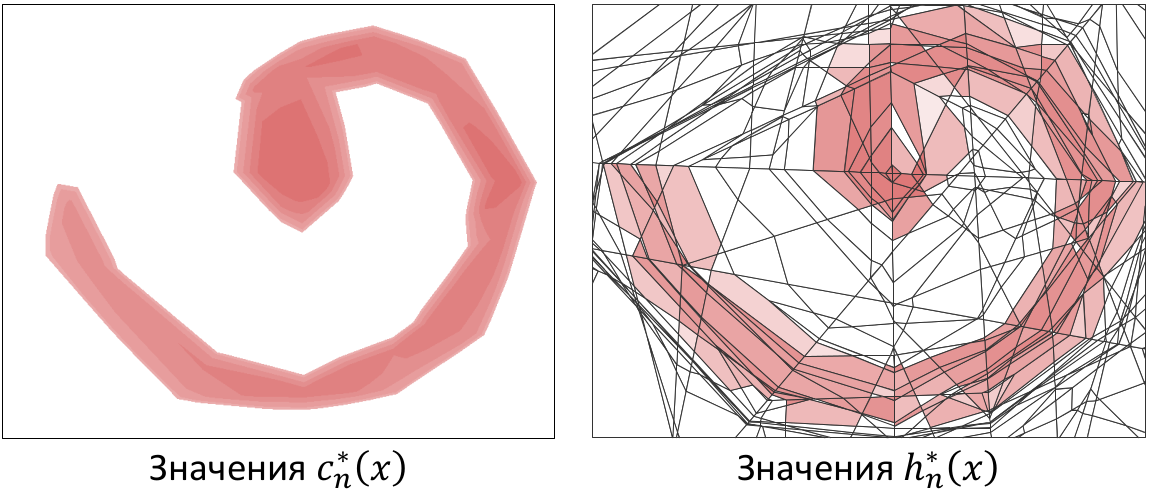
\includegraphics[width=0.9\linewidth]{Dissertation/images/ch1/application/cn_vs_hn.png}
    }
    \caption{Визуальное сравнение функций нейросетевой и гистограммной регрессий}
    \label{fig:cn_vs_hn}
\end{figure}

%%%%%%%%%%%%%%%%%%%%%%%%%%%%%%%%%%%%%%%%%%%%%%%%%%%%%%%%%%%%%%%%%%%%%%%%%%%%%%%%%%%%%%%%%%%%%%%%%%%%%%%%%%%%%%%
\subsection{Отказ от распознавания и интерпретация выходов}

Добавление фона позволяет не только лучше моделировать границу классов, но и реализовать механизм отказа от распознавания: наблюдения, попадающие в области низкой плотности, классифицируются как ``неизвестные``. Это открывает путь к более гибкому принятию решений -- например, маркированию таких примеров для дополнительного анализа или анализа дополнительных признаков.

%%%%%%%%%%%%%%%%%%%%%%%%%%%%%%%%%%%%%%%%%%%%%%%%%%%%%%%%%%%%%%%%%%%%%%%%%%%%%%%%%%%%%%%%%%%%%%%%%%%%%%%%%%%%%%%
\subsection{Влияние порога доверия на характеристики классификатора}
В рамках предложенного подхода в качестве дополнительного механизма контроля за качеством классификации вводится параметр \(\beta \in [0, 1)\), интерпретируемый как порог доверия. Значение \(\beta\) используется для принятия решения о классификации наблюдения: если значение выхода модели по модулю не превышает \(\beta\), классификатор воздерживается от принятия решения, т.е. формирует отказ от распознавания.

Введение порога \(\beta\) позволяет контролировать баланс между полнотой и надёжностью классификационных решений. При низких значениях \(\beta\) классификатор склонен выдавать решения по всем поступающим наблюдениям, включая случаи с высокой неопределённостью. При этом возрастает риск ошибочной классификации, особенно вблизи границ разделяющих поверхностей. Повышение значения \(\beta\) ведёт к росту количества отказов от распознавания, но одновременно повышает достоверность решений по тем наблюдениям, для которых классификация всё же производится.

На рисунке~\cref{fig:beta_thresholds} приведена визуализация результатов классификации при различных значениях порога \(\beta\): от 0 (классификация осуществляется по всем наблюдениям) до 0.5 (классификатор выдаёт решение только в случаях высокой уверенности). Видно, что при увеличении \(\beta\) область отказов расширяется (обозначена белым цветом), что соответствует желаемому поведению системы в условиях ограниченной уверенности модели.

\begin{figure}[ht]
    \centerfloat{
        \hfill
        \subcaptionbox{\(\beta = 0\)}{%
            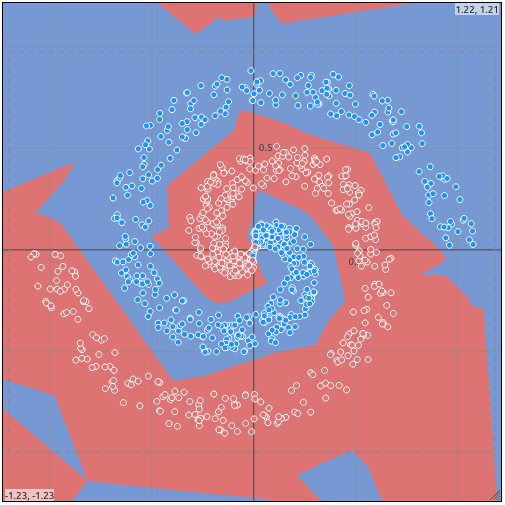
\includegraphics[width=0.24\linewidth]{Dissertation/images/ch1/application/beta0.0.png}}
        \hfill
        \subcaptionbox{\(\beta = 0.1\)}{%
            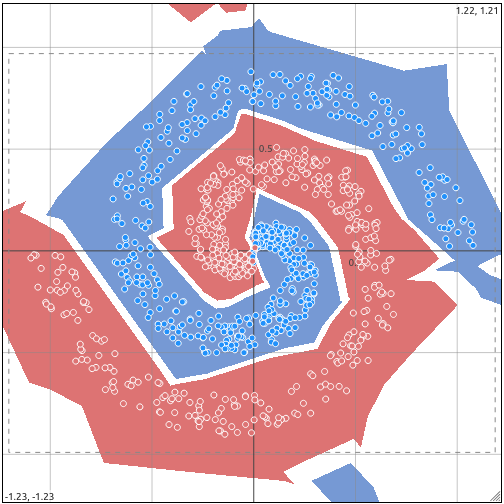
\includegraphics[width=0.24\linewidth]{Dissertation/images/ch1/application/beta0.1.png}}
        \hfill
        \subcaptionbox{\(\beta = 0.3\)}{%
            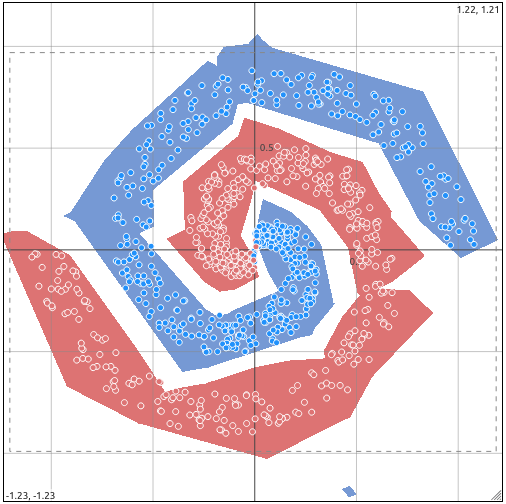
\includegraphics[width=0.24\linewidth]{Dissertation/images/ch1/application/beta0.3.png}}
        \hfill
        \subcaptionbox{\(\beta = 0.5\)}{%
            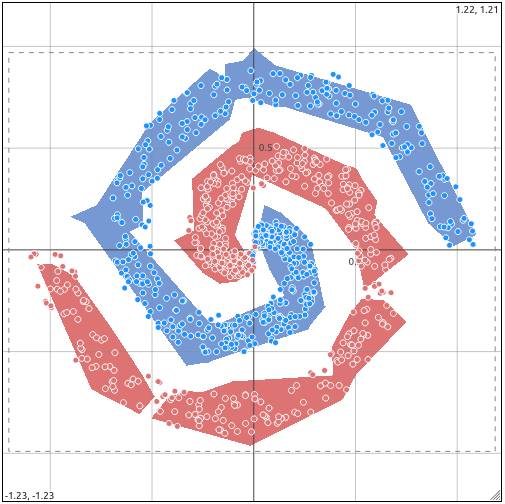
\includegraphics[width=0.24\linewidth]{Dissertation/images/ch1/application/beta0.5.png}}
        \hfill
    }
    \caption{Влияние порога доверия \(\beta\) на пространственное распределение классификационных решений}
    \label{fig:beta_thresholds}
\end{figure}

%%%%%%%%%%%%%%%%%%%%%%%%%%%%%%%%%%%%%%%%%%%%%%%%%%%%%%%%%%%%%%%%%%%%%%%%%%%%%%%%%%%%%%%%%%%%%%%%%%%%%%%%%%%%%%%
\subsection{Выводы}

Модификация бинарного классификатора позволяет существенно улучшить устойчивость и надёжность модели, основанной на многослойном персептроне. Примеры наглядно показывают, что обучение на расширенном наборе данных с добавлением фона позволяет реализовать отказ от распознавания вне носителя данных, повысить устойчивость к некоторым видам атак, а также сделать предположение о связи между функциями нейросетевой и гистограммной регрессии.

           % Глава 1
\chapter{Унарная классификация}

\section{Модель кластеров уровня плотности}

Одним из фундаментальных подходов к выявлению скрытой структуры в данных является использование модели кластеров уровня плотности. Этот подход берёт своё начало в работах \cite{bock1974automatische} и \cite{hartigan1975clustering}, в которых было предложено рассматривать кластеры как области пространства признаков, характеризующиеся повышенной плотностью вероятностного распределения. Интуитивно предполагается, что наблюдения, принадлежащие к одному кластеру, с большей вероятностью сосредоточены в определённой области пространства, в то время как между кластерами плотность стремится к более низким значениям.

В дальнейшем, развитие этой идеи получило формальное обоснование в рамках непараметрических методов оценивания плотности. В частности, в работах~\cite{devroye1980strong} и \cite{devroye1977strong} были представлены строгие доказательства состоятельности таких оценок, как гистограмма, оценка по методу \(k\) ближайших соседей, а также ядерная оценка. Эти результаты впоследствии были систематизированы и обобщены в их монографии по непараметрической статистике, ставшей классической.

На основе этих теоретических результатов в~\cite{wong1983kth} предложили алгоритм кластеризации, основанный на выделении областей высокой плотности, который был реализован в рамках иерархического подхода. Этот метод, получивший название вероятностного метода, позволял строить деревья кластеров на основе последовательного объединения областей с близкими характеристиками плотности. К сожалению, из-за высокой вычислительной сложности, связанной с необходимостью многократного расчёта расстояний между точками и хранения оценок плотности в памяти, его практическое применение оказалось ограниченным малыми объёмами выборок и невысокой размерностью пространства признаков.

Формально, пусть \(f(X)\) -- плотность распределения случайного вектора \(X \in \mathbb{R}^d\). Для любого порогового значения \(c > 0\) вводится \textbf{множество уровня плотности}:
\[
B(c) = \{X \in \mathbb{R}^d : f(X) > c\}.
\]

Это множество представляет собой объединение всех точек, в которых плотность превышает заданное значение \(c\). Модель кластеров уровня плотности предполагает, что каждый кластер соответствует одной связной компоненте множества \(B(c)\):
\[
B(c) = \bigcup_{i=1}^M B_i(c),
\]
где \(B_1(c), B_2(c), \dots, B_M(c)\) -- непересекающиеся связные компоненты, каждая из которых интерпретируется как отдельный кластер.

Данный подход позволяет не задавать количество кластеров заранее, поскольку число связных компонент может изменяться в зависимости от значения \(c\). При больших значениях \(c\) в множестве \(B(c)\) остаются лишь точки, расположенные в наиболее плотных участках пространства, а при уменьшении \(c\) связные области начинают расширяться и объединяться, формируя иерархическую структуру кластеров.

На практике множество \(B(c)\) и его компоненты \(B_i(c)\) недоступны напрямую, поскольку истинная плотность \(f(X)\) неизвестна. Однако с использованием непараметрических оценок плотности можно построить приближённое множество уровня и использовать его для выявления кластеров. Это позволяет задать концептуальную основу для методов обучения без учителя, в которых наличие плотностной структуры в данных служит основой для группировки наблюдений.

Таким образом, модель кластеров уровня плотности обеспечивает строгую вероятностную интерпретацию кластеризации как задачи геометрического разделения множества высокого уровня плотности. Это становится особенно важным в ситуациях, когда отсутствуют априорные сведения о принадлежности объектов к классам, а само разделение должно быть основано исключительно на свойствах распределения наблюдаемых данных.

\section{Нейросетевая регрессия (случай одного класса)}

Как отмечалось в разделе~\cref{subsec:ch1/neural_approximation}, многослойный персептрон с кусочно-линейной функцией активации (в частности, с активацией вида \(|x|\)), при наличии \(L\) скрытых слоёв, каждый из которых содержит \(k\) нейронов, способен осуществлять \(\epsilon\)-приближенную аппроксимацию любой непрерывной функции на компакте. При этом конструкция такой нейросети задаёт иерархическое (по слоям) разбиение компакта \([0, 1]^d\) на \(O(k^{dL})\) ячеек, внутри которых выход нейросети представляет собой линейную функцию. Вычисление значения такой нейросети в произвольной точке \(x \in [0, 1]^d\) требует только последовательного выполнения операций скалярного умножения и сравнения, что обеспечивает высокую вычислительную эффективность полученной модели.

Для дальнейшего анализа введём обобщённую задачу регрессии, сформулированную следующим образом. Пусть имеется исходный набор наблюдений \(\{X_i\}_{i=1}^n\), представляющий собой независимые одинаково распределённые случайные величины на компакте \([0, 1]^d\) с неизвестной ограниченной плотностью распределения \(f(X)\). Этот набор можно интерпретировать как наблюдения некоторого целевого процесса, подлежащего моделированию. Для каждого такого наблюдения \(X_i\) положим значение метки \(Y_i = 1\).

Дополнительно сформируем ``фоновые`` наблюдения \(\{X_i\}_{i=n+1}^{2n}\), представляющие собой независимые одинаково распределённые случайные величины с равномерной плотностью распределения \(p(X)\) на том же компакте \([0,1]^d\). Для этих наблюдений положим значения \(Y_i = 0\). В результате будет получен комбинированный набор данных \(\{(X_i, Y_i)\}_{i=1}^{2n}\) мощности \(2n\).

Рассмотрим теперь задачу построения аппроксимирующей полносвязной нейросети \(c_n(X)\), решающей задачу регрессии в классе моделей фиксированной сложности, аналогичную задаче \cref{eq:perceptron_optimization}. Требуется найти такую нейросеть \(c_n^*(X)\), минимизирующую среднеквадратичную ошибку на объединённом наборе данных:

\begin{equation}
    \label{eq:unary_perceptron_optimization}
    \sum_{i=1}^{2n} \left(c_n(X_i) - Y_i\right)^2 \rightarrow \min_{c_n},
\end{equation}

\noindent где минимум берётся по всем полносвязным нейросетям, общее число нейронов в которых не превышает заданного порогового значения \(kL + 1\).

Пусть в результате построения \(c_n^*(X)\) на компакте \([0, 1]^d\) получено разбиение на \(N\) ячеек \(K = \{K_1, K_2, \dots, K_N\}\). Введём далее кусочно-постоянную функцию \(h_n(X)\), принимающую постоянные значения внутри каждой ячейки \(K_r\), и сформулируем задачу приближённой оценки вероятности принадлежности наблюдения классу \(Y = 1\) в виде:

\begin{equation}
    \label{eq:unary_histogram_optimization}
    \sum_{i=1}^{2n} \left(h_n(X_i) - Y_i\right)^2 \rightarrow \min_{h_n}
\end{equation}

Как и в \cref{eq:histogram_optimization}, задача~\cref{eq:unary_histogram_optimization} может быть решена независимо в каждой ячейке \(K_r\), при этом оптимальное значение \(h_n^*(X)\) в данной ячейке определяется соотношением:

\begin{equation}
    h_n^*(X) = \frac{n_1(X)}{n_1(X) + n_0(X)},
\end{equation}

\noindent где \(n_1(X)\) -- количество наблюдений с меткой \(Y = 1\) в ячейке, содержащей точку \(X\), а \(n_0(X)\) -- количество фоновых наблюдений (с меткой \(Y = 0\)) в той же ячейке.

Пример вычисления функции гистограммной регрессии показан на рисунке~\cref{fig:unary_histogram_evaluation}.

\begin{figure}[ht]
    \centerfloat{
        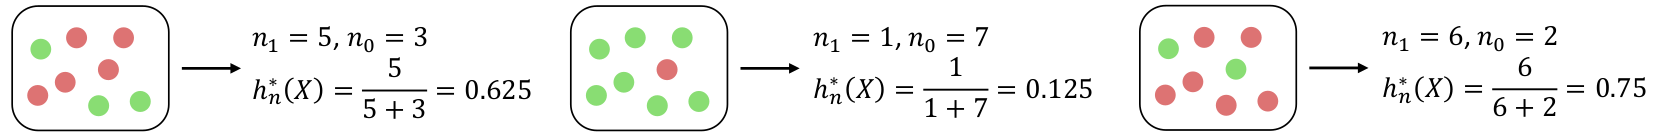
\includegraphics[width=\linewidth]{Dissertation/images/ch1/bayesian_classifier_approximation/histogram_evaluation.png}
    }
    \caption{Пример вычисления \(h_n^*(X)\) в некоторой ячейке \(K_r\) в унарном случае}
    \label{fig:unary_histogram_evaluation}
\end{figure}

Полученная функция \(h_n^*(X)\) представляет собой оценку апостериорной вероятности принадлежности к целевому распределению \(f(X)\), основанную на локальной структуре данных в разбиении, индуцированном нейросетевой аппроксимацией.
\section{Нейросетевая регрессия как оценка апостериорной вероятности класса}

Рассмотрим гистограммные оценки плотности для двух классов:

\[
f_n(X) = \frac{n_1(X)}{n \cdot V(K_r)}, \quad p_n(X) = \frac{n_0(X)}{n \cdot V(K_r)},
\]

\noindent где \(V(K_r)\) -- мера ячейки \(K_r\).

На основе этих оценок можно определить байесовскую аппроксимацию апостериорной вероятности класса:
\[
h_n^*(X) = \frac{f_n(X)}{f_n(X) + p_n(X)}.
\]

Зададим порог \(\beta \in [0, 1)\). Тогда неравенство \(h_n^*(X) > \beta\) позволяет выделить из множества \(K\) ячейки с высоким значением выборочной оценки апостериорной вероятности класса \(+1\). Преобразуя выражение, получим эквивалентную форму~\cite{mitsobi2025}:
\[
f_n(X) > \frac{\beta}{1 - \beta} \cdot p_n(X).
\]

Иными словами, объект \(X\) попадает в область пространства признаков, где плотность первого класса превышает плотность фонового класса более чем в \(\frac{\beta}{1 - \beta}\) раз. Это условие можно использовать для выделения из множества ячеек \(\{K_1, K_2, \ldots, K_N\}\) подмножества, соответствующего кластеру высокой плотности. Такие области могут рассматриваться как выборочные приближения к области, поддерживающей плотность распределения первого класса.

По аналогии с разделом~\cref{sec:ch1/hist_neural_approximations}, согласно результатам работы~\cite{devroye2013probabilistic}, для обеспечения статистической состоятельности гистограммных оценок плотности необходимо, чтобы с ростом объёма обучающей выборки происходило соответствующее увеличение числа нейронов в аппроксимирующей сети. Это условие отражает потребность в возрастающем разрешении пространства признаков, необходимом для точного приближения апостериорной вероятности.

В таком случае для решения о принадлежности нового наблюдения \(X\) области высокой плотности достаточно проверить выполнение неравенства \(c_n^*(X) > \beta\), что представляет собой гораздо более простую с вычислительной точки зрения операцию, чем вычисление \(h_n^*(X)\).

Таким образом, задача принятия решения сводится к сравнению выхода нейросети с порогом, что обеспечивает линейную по числу слоёв и нейронов вычислительную сложность и устраняет необходимость работы с явным представлением плотностей. Это делает метод особенно привлекательным в задачах, требующих масштабируемости и эффективности при обработке новых входных данных.

\section{Случай нескольких классов}

В случае многоклассовой классификации (\(C > 2\)) предлагаемая конструкция унарных классификаторов сохраняет свою применимость и обладает рядом существенных преимуществ по сравнению с классическим подходом, основанным на многоклассовой нейронной сети или на парных классификаторах ``один против одного''. Прежде всего, при использовании унарной схемы для каждого класса \(c = 1, \dots, C\) строится собственный унарный классификатор, обученный различать носитель класса \(c\) от фонового равномерного распределения.

Таким образом, требуется построить \(C\) независимых классификаторов, каждый из которых решает задачу бинарной классификации в формате ``объекты данного класса против фона''. В отличие от схемы ``один против одного'', где количество классификаторов составляет \(\frac{C(C - 1)}{2}\), унарная схема масштабируется линейно по числу классов и не требует сложных стратегий агрегации результатов голосования.

\section{Преимущества унарной классификации}

Ключевым достоинством унарного подхода является полная устойчивость к проблеме дисбаланса классов. Каждый классификатор обучается только на положительных объектах своего класса и на независимом фоновом множестве, совпадающим по размеру. Таким образом, влияние других, возможно многочисленных, классов исключается на этапе обучения, и несбалансированность исходного обучающего множества не приводит к смещению в сторону более представленных классов.

Кроме того, каждый классификатор формирует свою собственную аппроксимацию апостериорной вероятности \(c_n^{(i)}(x)\), оценивая степень принадлежности точки \(x\) классу \(i\). Совокупность таких значений \((c_n^{(1)}(x), \dots, c_n^{(C)}(x))\) образует векторную оценку, позволяющую как выбрать наиболее вероятный класс (например, по максимуму), так и сформулировать стратегию отказа, если все оценки не превышают заданного порога \(\beta\). Последнее обеспечивает возможность построения отказоустойчивой классификационной системы, способной помечать сомнительные случаи как требующие дополнительного рассмотрения.

Ещё одним немаловажным преимуществом является модульность архитектуры: поскольку все классификаторы независимы, допускается использование различной архитектуры (в том числе различной глубины и сложности) для различных классов. Это даёт возможность адаптировать модель под особенности каждого из классов, делая систему более гибкой и устойчивой к неоднородности обучающих данных.

\section{Оценка качества унарных классификаторов}

При оценке качества стандартных многоклассовых классификаторов традиционно используют метрики точности, полноты, \(F_1\)-score и аналогичные~\cite{obi2023comparative}. Однако в контексте унарной классификации такие показатели оказываются недостаточно информативными, так как каждый классификатор в унарной схеме обучается независимо и ориентирован на различение своего целевого класса от фонового распределения. В частности, стандартная точность не учитывает случаи ``отказа'' классификатора (когда выход нейросети не превышает порог \(\beta\)), а \(F_1\)-score и подобные метрики не отражают взаимное влияние классификаторов при многоклассовой интерпретации.

Для более детальной оценки работы унарного классификатора предлагается рассматривать три дополнительных свойства: мощность, эффективность и меру неразделимости классов.

\subsection{Мощность классификатора}

Мощность классификатора \(c^{(i)}(x)\) определяется как доля точек целевого класса \(i\), принимаемых классификатором, то есть для которых выходная аппроксимация апостериорной вероятности превышает заданный порог \(\beta\). Формально для двух классов показатели вычисляются следующим образом:

\[
n^{(1)}_1 = \sum_{i=1}^{n^{(1)}} \mathbb{I}_{\{c^{(1)}(x_i) \geq \beta\}}, \quad 
n^{(2)}_2 = \sum_{i=1}^{n^{(2)}} \mathbb{I}_{\{c^{(2)}(x_i) \geq \beta\}},
\]

\[
p^{(1)} = \frac{n^{(1)}_1}{n^{(1)}}, \quad
p^{(2)} = \frac{n^{(2)}_2}{n^{(2)}},
\]
где \(n^{(1)}\) и \(n^{(2)}\) -- количество наблюдений классов 1 и 2 соответственно. Мощность позволяет оценить долю объектов класса, корректно распознанных классификатором без отказа, и является базовой характеристикой ``чувствительности'' модели к своему классу.

Для получения интегральной характеристики мощности всей пары классификаторов можно использовать гармоническое среднее:

\[
P_{12} = \frac{2 p^{(1)} p^{(2)}}{p^{(1)} + p^{(2)}}.
\]

Метрика \(P_{12}\) отражает общую способность пары классификаторов корректно распознавать свои классы. При этом, если один из классификаторов имеет низкую мощность, интегральная метрика также будет снижена, что интуитивно соответствует снижению общей чувствительности системы.


\subsection{Эффективность классификатора}

Эффективность характеризует способность классификатора корректно выделять объекты своего класса относительно других классификаторов. Для двух классов вводятся следующие показатели:

\[
n^{(1)}_{10} = \sum_{i=1}^{n^{(1)}} \mathbb{I}_{\{c^{(1)}(x_i) \geq \beta \wedge c^{(2)}(x_i) < \beta\}}, \quad
n^{(2)}_{02} = \sum_{i=1}^{n^{(2)}} \mathbb{I}_{\{c^{(2)}(x_i) \geq \beta \wedge c^{(1)}(x_i) < \beta\}},
\]

\[
e^{(1)} = \frac{n^{(1)}_{10}}{n^{(1)}}, \quad e^{(2)} = \frac{n^{(2)}_{02}}{n^{(2)}}.
\]

Показатели качества классификатора \(e^{(i)}\) отражают долю объектов, корректно распознанных своим классификатором и отвергнутых чужим(и). На их основе определяется интегральная метрика эффективности:

\[
E_{12} = \frac{2 e^{(1)} e^{(2)}}{e^{(1)} + e^{(2)}}.
\]

Метрика \(E_{12}\) аналогична гармоническому среднему и позволяет количественно оценить согласованность работы классификаторов при минимизации взаимных ошибок.


\subsection{Мера неразделимости классов}

Для количественной оценки степени пересечения областей, признанных обоими классификаторами, вводится понятие меры неразделимости классов. Внутренние показатели, характеризующие долю объектов, которые одновременно принимаются обоими классификаторами, интерпретируются как свойство наплываемости классов:

\[
n^{(1)}_{12} = \sum_{i=1}^{n^{(1)}} \mathbb{I}_{\{c^{(1)}(x_i) \geq \beta \wedge c^{(2)}(x_i) \geq \beta\}}, \quad
n^{(2)}_{12} = \sum_{i=1}^{n^{(2)}} \mathbb{I}_{\{c^{(2)}(x_i) \geq \beta \wedge c^{(1)}(x_i) \geq \beta\}},
\]

\[
g^{(1)} = \frac{n^{(1)}_{12}}{n^{(1)}}, \quad g^{(2)} = \frac{n^{(2)}_{12}}{n^{(2)}},
\]

На основе этих показателей определяется интегральная мера неразделимости классов:

\[
G_{12} = \frac{2 g^{(1)} g^{(2)}}{g^{(1)} + g^{(2)}}.
\]

Метрика \(G_{12}\) отражает, насколько сильно области, распознаваемые различными классификаторами, перекрываются. Высокое значение \(G_{12}\) свидетельствует о значительном наплывании классов друг на друга и, следовательно, о потенциальной сложности их разделения в пространстве признаков.


\subsection{Визуализация метрик}

Для иллюстрации поведения предложенных метрик рассмотрены три модельные ситуации и описаны значения интегральных показателей мощности, эффективности и меры неразделимости классов. Для сопоставления приведены также значения стандартных метрик бинарной классификации (accuracy, precision, recall, \(F_1\)).  

\begin{enumerate}
    \item \textbf{Два разнесённых гауссиана}. Классы линейно разделимы (рисунок~\cref{fig:metrics_cases}\subcaptionref{fig:metrics_cases_ideal}). Мощности обоих классификаторов равны единице (\(p^{(1)}=p^{(2)}= 1\)), эффективность также равна единице (\(E_{12} = 1\)), мера неразделимости равна нулю (\(G_{12} = 0\)). Классические метрики accuracy, precision, recall и \(F_1\) также принимают значение 1.  

    \item \textbf{Три гауссиана с вложением одного класса в другой}. Второй класс полностью лежит внутри первого (рисунок~\cref{fig:metrics_cases}\subcaptionref{fig:metrics_cases_one_inside}). Мощность первого классификатора равна 1, второго -- равна 0 (\(p^{(1)} = 1\), \(p^{(2)}=0\)), интегральный показатель мощности \(P_{12} = 0\). Эффективность первого классификатора равна 0.5, второго — 0 (\(e^{(1)} = 0.5\), \(e^{(2)} = 0\)), что даёт \(F_{12}=0\). Наплываемость первого классификатора равна 0.5, второго -- 1, интегральная мера неразделимости \(G_{12} = 0.75\). Для стандартных метрик accuracy, precision, recall и \(F_1\) равны \(2/3\).  

    \item \textbf{Два полностью совпадающих гауссиана}. Классы неразделимы (рисунок~\cref{fig:metrics_cases}\subcaptionref{fig:metrics_cases_identical}). Мощность обоих классификаторов равна нулю (\(p^{(1)} = p^{(2)} = 0\)), что даёт \(P_{12} = 0\). Эффективность также равна нулю (\(F_{12}=0\)). Наплываемость обоих классификаторов максимальна (\(G_{12} = 1\)). При этом accuracy, precision, recall и \(F_1\) принимают значение 0.5.
\end{enumerate}

\begin{figure}[ht]
    \centerfloat{
        \hfill
        \subcaptionbox{разделимые классы\label{fig:metrics_cases_ideal}}{%
            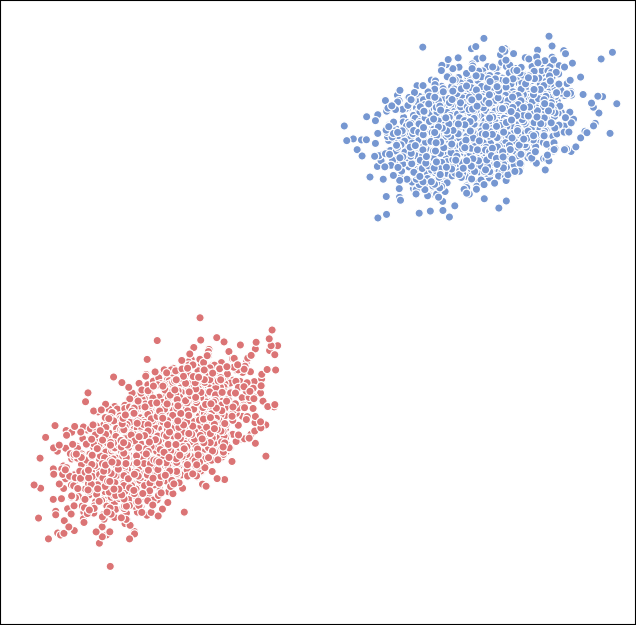
\includegraphics[width=0.3\linewidth]{Dissertation/images/ch2/metrics/ideal.png}}
        \hfill
        \subcaptionbox{второй класс вложен в первый\label{fig:metrics_cases_one_inside}}{%
            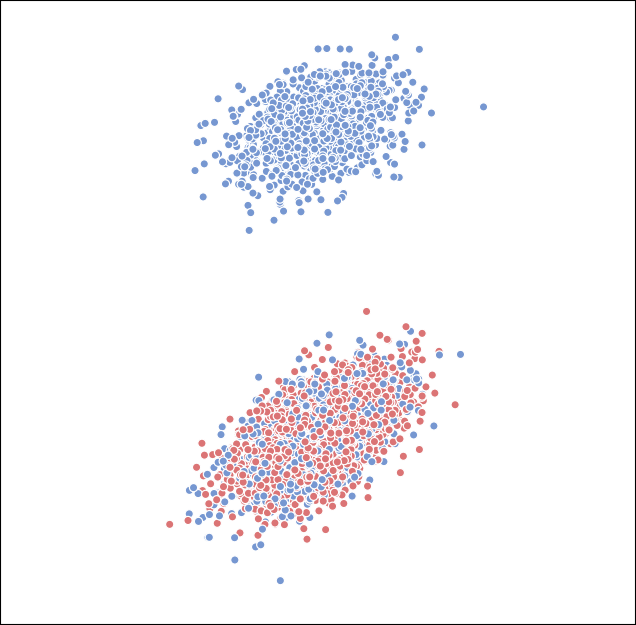
\includegraphics[width=0.3\linewidth]{Dissertation/images/ch2/metrics/second_inside.png}}
        \hfill
        \subcaptionbox{совпадающие классы\label{fig:metrics_cases_identical}}{%
            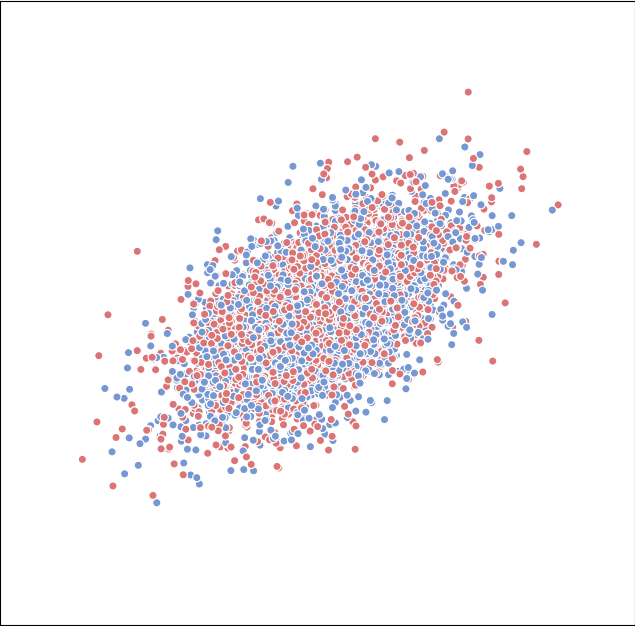
\includegraphics[width=0.3\linewidth]{Dissertation/images/ch2/metrics/identical.png}}
        \hfill
    }
    \caption{Модельные ситуации для анализа метрик}
    \label{fig:metrics_cases}
\end{figure}

Таким образом, видно, что предложенные показатели позволяют различать случаи, в которых стандартные метрики дают одинаковые значения, но интерпретация существенно различается.

\subsection{Обобщение на многоклассовый случай}

Для системы из \(C > 2\) унарных классификаторов аналогичные метрики могут быть вычислены попарно для каждой пары классификаторов, что позволяет получить полную картину взаимодействия классов. В то же время для оценки качества отдельных классификаторов достаточно использовать показатели мощности, а для анализа пересечений и эффективности -- соответствующие обобщённые гармонические средние по всем парам. Такой подход обеспечивает более информативную и детализированную оценку по сравнению с традиционными многоклассовыми метриками и учитывает особенности работы унарной схемы: независимость классификаторов, возможность отказа и линейную масштабируемость по числу классов.

\section{Иллюстрация работы на модельных примерах}

Для наглядной демонстрации описанного подхода были построены унарные классификаторы для одного, двух и четырёх классов на модельных данных. В каждом случае в качестве фона использовались равномерно распределённые точки на единичном квадрате \([0, 1]^2\), а положительные объекты представляли собой выборки из компактных, хорошо различимых распределений.

На рисунке~\cref{fig:unary_one} показана граница принятия решения, построенная унарным классификатором для одного класса. Видно, что модель успешно выделяет область высокой плотности положительного класса, отсекая фон.

\begin{figure}[ht]
    \centerfloat{
        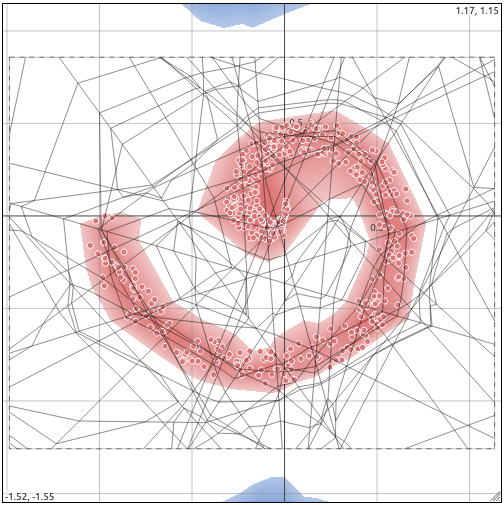
\includegraphics[width=0.9\linewidth]{Dissertation/images/ch2/usage/unary1.png}
    }
    \caption{Оценка плотности одного класса с использованием унарной схемы}
    \label{fig:unary_one}
\end{figure}

На рисунке~\cref{fig:unary_two} приведены результаты построения двух независимых унарных классификаторов для двух классов. Каждый классификатор определяет свою область плотности, и итоговая классификация осуществляется по наибольшей из двух аппроксимаций.

\begin{figure}[ht]
    \centerfloat{
        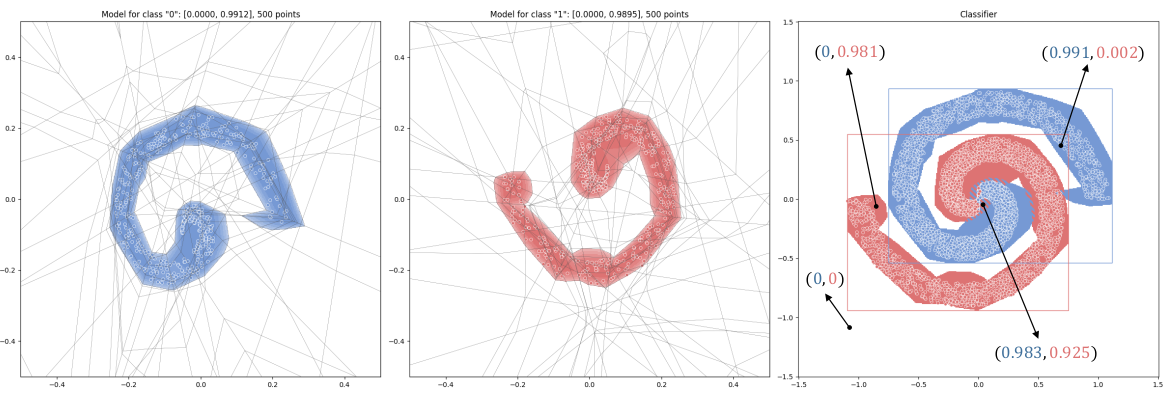
\includegraphics[width=\linewidth]{Dissertation/images/ch2/usage/unary2.png}
    }
    \caption{Унарная классификация для двух классов}
    \label{fig:unary_two}
\end{figure}

Наиболее показательный случай -- построение унарных классификаторов для четырёх классов с искусственно созданным дисбалансом. Один из классов содержит в семь раз больше наблюдений, чем другой, ещё один -- в пять раз больше и ещё один в три раза больше. Тем не менее, благодаря независимому обучению каждого классификатора на своём классе и фоновом множестве, области плотности получаются хорошо различимыми и не искаженными из-за дисбаланса. Это подтверждает устойчивость метода к нарушению пропорций классов (рисунок~\cref{fig:unary_four}).

\begin{figure}[ht]
    \centerfloat{
        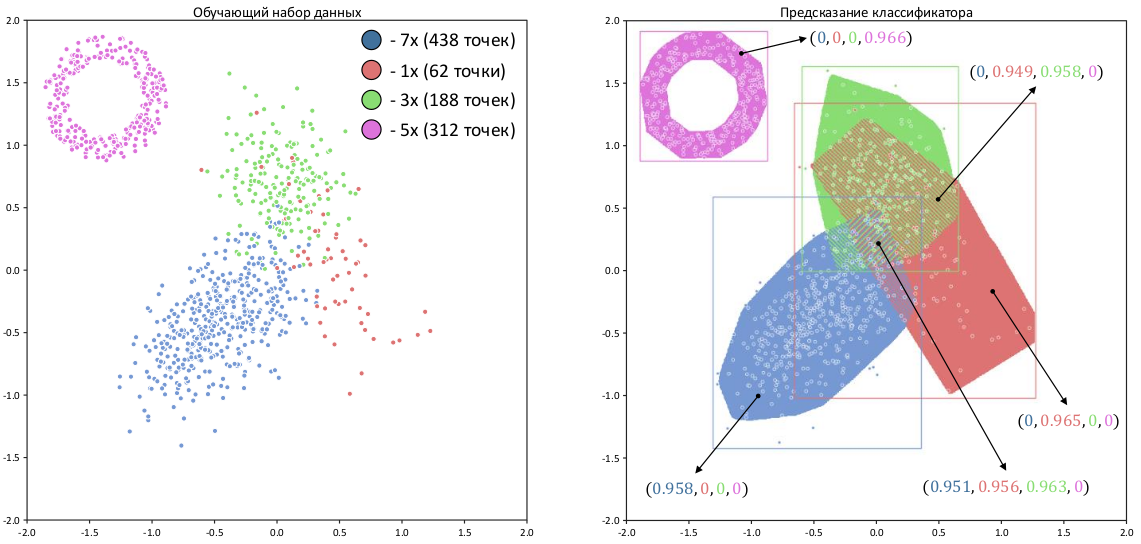
\includegraphics[width=\linewidth]{Dissertation/images/ch2/usage/unary4.png}
    }
    \caption{Унарная классификация для четырёх классов с дисбалансом}
    \label{fig:unary_four}
\end{figure}

Таким образом, предложенная схема построения унарных классификаторов позволяет надёжно и интерпретируемо решать задачу многоклассовой классификации, не требуя дополнительных допущений о балансе данных или единой архитектуре модели. Векторная оценка апостериорных вероятностей предоставляет дополнительную гибкость и возможность построения сложных решений с механизмами отказа или уточнения.
           % Глава 2
\chapter{Применение унарной классификации}

\section{Построение репродукционных выборок}

\fixme{ДОПИСАТЬ ПРО РЕПРОДУКЦИЮ ПО ГИСТОГРАММЕ}

Одним из ключевых применений унарной классификации является задача создания синтетических табличных данных, особенно актуальная в условиях ограниченного доступа к реальным данным. Такие ограничения~\cite{gal2023synthetic} могут быть обусловлены законодательными мерами по защите персональных данных~\cite{joshi2024synthetic}, коммерческой тайной или просто недостаточным объёмом исходной выборки. Синтетические данные находят применение в обучении моделей, увеличении объёма обучающих данных~\cite{belyaeva2020synthetic}, обеспечении воспроизводимости научных исследований~\cite{grund2022using} и безопасной передаче информации между организациями.

Основное требование к синтетическим данным -- сохранение статистических и структурных свойств оригинального распределения при гарантии отсутствия утечки чувствительной информации \cite{bauer2024comprehensive}. На практике это означает, что синтетические выборки должны отражать ту же плотность вероятности, что и оригинальные данные, при этом исключая прямое копирование реальных наблюдений.

Для генерации синтетических данных применяются как классические статистические методы, так и модели, основанные на машинном обучении~\cite{figueira2022survey} -- например, вариационные автоэнкодеры (VAE)~\cite{wan2017variational}, генеративно-состязательные сети (GAN)~\cite{jordon2018pate}, диффузионные модели~\cite{villaizan2024diffusion} и др. \cite{akkem2024comprehensive}. Статистические методы обеспечивают согласованность оценок -- то есть, при росте объёма выборки оценка приближается к истинному распределению. В то же время, нейросетевые методы, несмотря на высокую эмпирическую эффективность, зачастую не обладают теоретическими гарантиями сохранения статистических свойств.

В работе \cite{synthetic2025unary} предлагается альтернативный подход к генерации синтетических данных, основанный на унарной классификации. В отличие от традиционных генеративных моделей, которые непосредственно генерируют новые объекты, здесь нейросеть обучается различать реальные точки данных и точки, равномерно сэмплированные из фонового распределения на ограниченной области пространства. В дальнейшем результат классификации используется для фильтрации вновь сгенерированных фоновых точек, формируя репродукционную выборку, приближающую плотность исходных данных.

\subsection{Постановка задачи}

Рассмотрим множество наблюдений \(X = \{x_1, x_2, \dots, x_n\} \in [0, 1]^d\), представляющее собой выборку из неизвестного распределения с плотностью \(f(x)\). Цель состоит в построении синтетической выборки \(\tilde{X} = \{\tilde{x}_1, \tilde{x}_2, \dots, \tilde{x}_m\}\), которая сохраняет статистические свойства оригинального распределения (рисунок~\cref{fig:synthetic_data_task}).

\begin{figure}[ht]
    \centerfloat{
        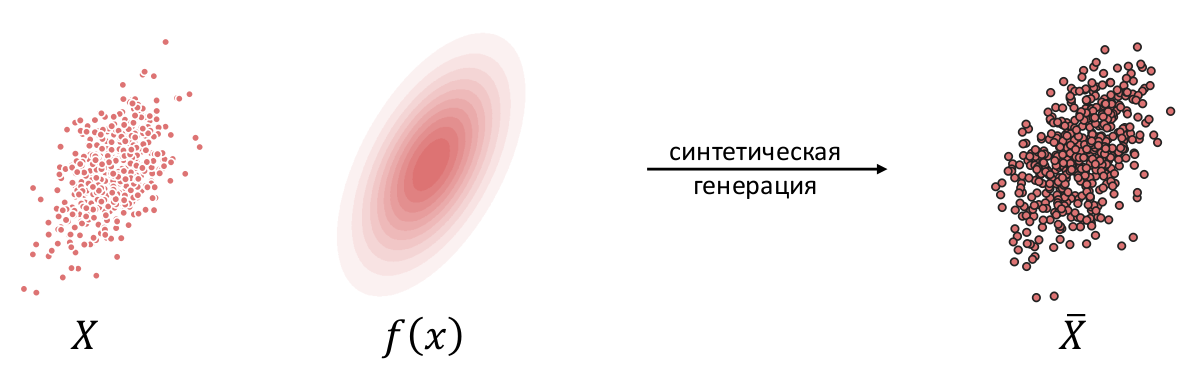
\includegraphics[width=\linewidth]{Dissertation/images/ch3/reproduction/synthetic_data_task.png}
    }
    \caption{Схематичное представление задачи создания синтетических данных}
    \label{fig:synthetic_data_task}
\end{figure}

Традиционные методы оценки плотности распределения обычно предполагают построение непараметрической оценки \(\hat{f}(x)\) для аппроксимации \(f(x)\). В отличие от этого, предлагается альтернативный подход, основанный на унарной классификации, где нейронная сеть обучается различать реальные точки данных и выборки, взятые из равномерного фонового распределения.

\subsection{Обучение классификатора}

В рамках предложенного подхода рассматривается фоновое распределение -- равномерное на компакте \([0, 1]^d\). Из него отбирается множество точек \(B = \{b_1, b_2, \dots, b_n\}\), равное по мощности множеству \(X\).

На объединённой выборке \(X \cup B\) унарно обучается многослойный персептрон \(c_n(x): [0, 1]^d \to [0, 1]\). Метки классов задаются следующим образом:
\[
\left\{
\begin{alignedat}{2}
    &&c_n(x) \rightarrow 1, \quad &\text{если } x \in X, \\
    &&c_n(b) \rightarrow 0, \quad &\text{если } b \in B, \\
\end{alignedat}
\right.
\]

Для обучения модели используется функция потерь среднеквадратичной ошибки (MSE):
\[
L = \sum_{x \in X} (1 - c_n(x))^2 + \sum_{b \in B} (0 - c_n(b))^2.
\]

Выбор MSE вместо кросс-энтропии обусловлен желанием получить гладкую аппроксимацию функции плотности. В отличие от кросс-энтропии, которая стремится к резкому разделению классов, MSE интерпретируется как регрессионная функция, позволяющая трактовать выход сети как сглаженную аппроксимацию плотности без необходимости нормировки.

Особенность метода -- генерация новых фоновых точек на каждом обучающем шаге (эпохе), а не фиксированное множество \(B\), заданное в начале. Это обеспечивает более полное покрытие области и снижает переобучение на конкретных фоновых примерах.

\subsection{Создание репродукционных данных}

После завершения обучения классификатора, синтетические данные получаются путём фильтрации новых фоновых точек. Из равномерного распределения на \([0, 1]^d\) сэмплируется множество \(\tilde{B}\), и каждая точка \(\tilde{b} \in \tilde{B}\) включается в итоговую выборку с вероятностью \(c_n(\tilde{b})\). То есть:
\[
\tilde{X} = \{ \tilde{b} \in \tilde{B} \mid \xi < c_n(\tilde{b}) \}, \quad \xi \sim \text{Uniform}(0,1).
\]

Такой подход позволяет строить выборку, приближенную к оригинальной плотности \( f(x) \), не предполагая явной генеративной модели. При этом плотность оценивается через классификационную задачу, что позволяет интерпретировать модель как адаптивную гистограмму.

\subsection{Экспериментальное исследование}

Для демонстрации эффективности метода проведены эксперименты на модельных датасетах с известной структурой (рисунок~\cref{fig:synthetic_datasets}). Это позволяет объективно оценить способность модели к воспроизведению статистических свойств. Рассматривались следующие выборки:

\begin{itemize}
  \item \textbf{Спираль}: двумерная выборка, где точки образуют спираль. Проверяется способность метода к моделированию нелинейной кластеризации.
  \item \textbf{Два квадрата}: два раздельных кластера квадратной формы. Оценивается сохранение пространственной структуры и разделимости.
  \item \textbf{Нормальное распределение}: двумерное распределение с известными параметрами. Проверяется соответствие ковариационной структуры.
  \item \textbf{Многомерное нормальное распределение}: 10-мерный аналог предыдущего случая, оценивающий качество генерации в высокоразмерном пространстве.
\end{itemize}

\begin{figure}[ht]
    \centerfloat{
        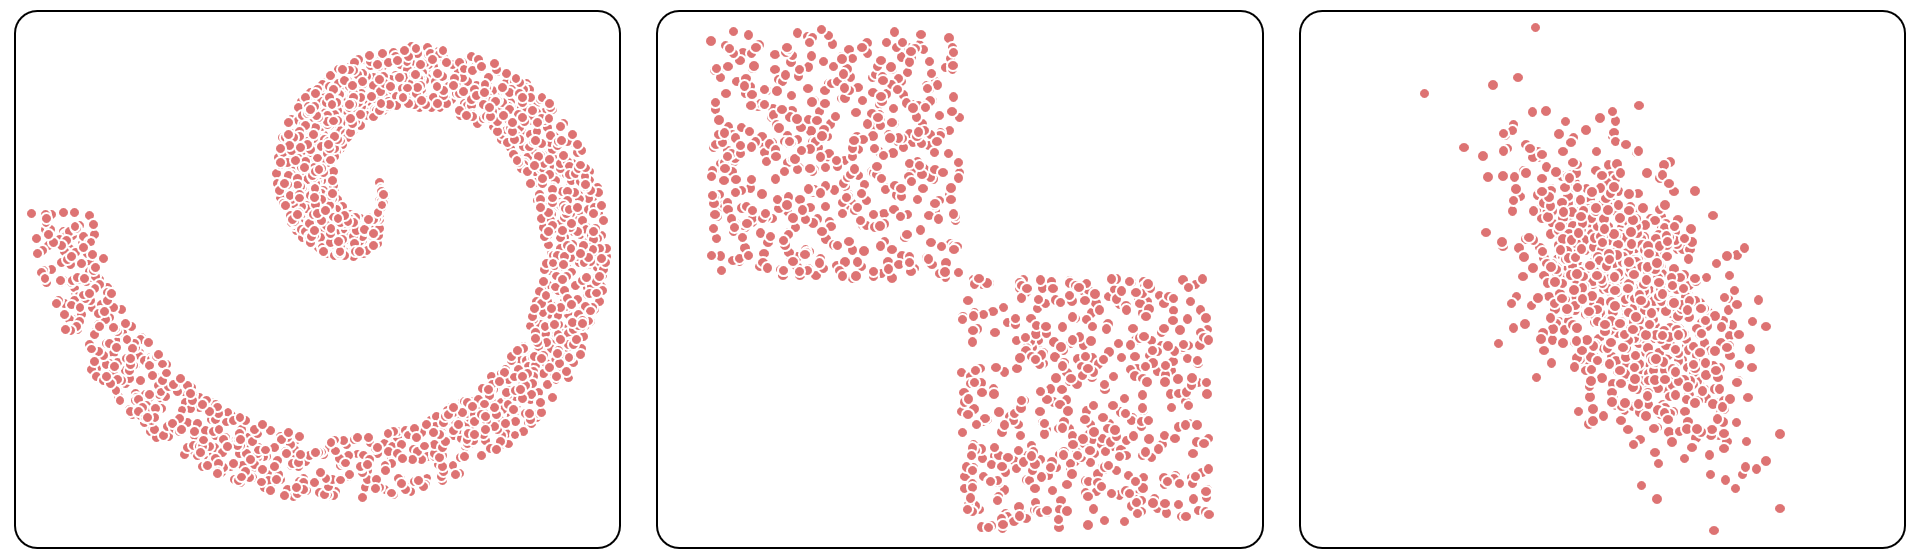
\includegraphics[width=\linewidth]{Dissertation/images/ch3/reproduction/datasets.png}
    }
    \caption{Использованные наборы данных для построения репродукционных выборок (спираль, два квадрата и гауссиан)}
    \label{fig:synthetic_datasets}
\end{figure}

Визуализация результатов (рисунок~\cref{fig:synthetic_results}) демонстрирует, что сгенерированные данные точно воспроизводят форму, плотность и вариативность оригинальных данных. В случае многомерного нормального распределения сохраняется ковариационная структура, хотя наблюдается небольшое увеличение дисперсии -- эффект, обусловленный ростом размерности и разрежённостью пространства.

\begin{figure}[ht]
    \centerfloat{
        \hfill
        \subcaptionbox{Спираль}{%
            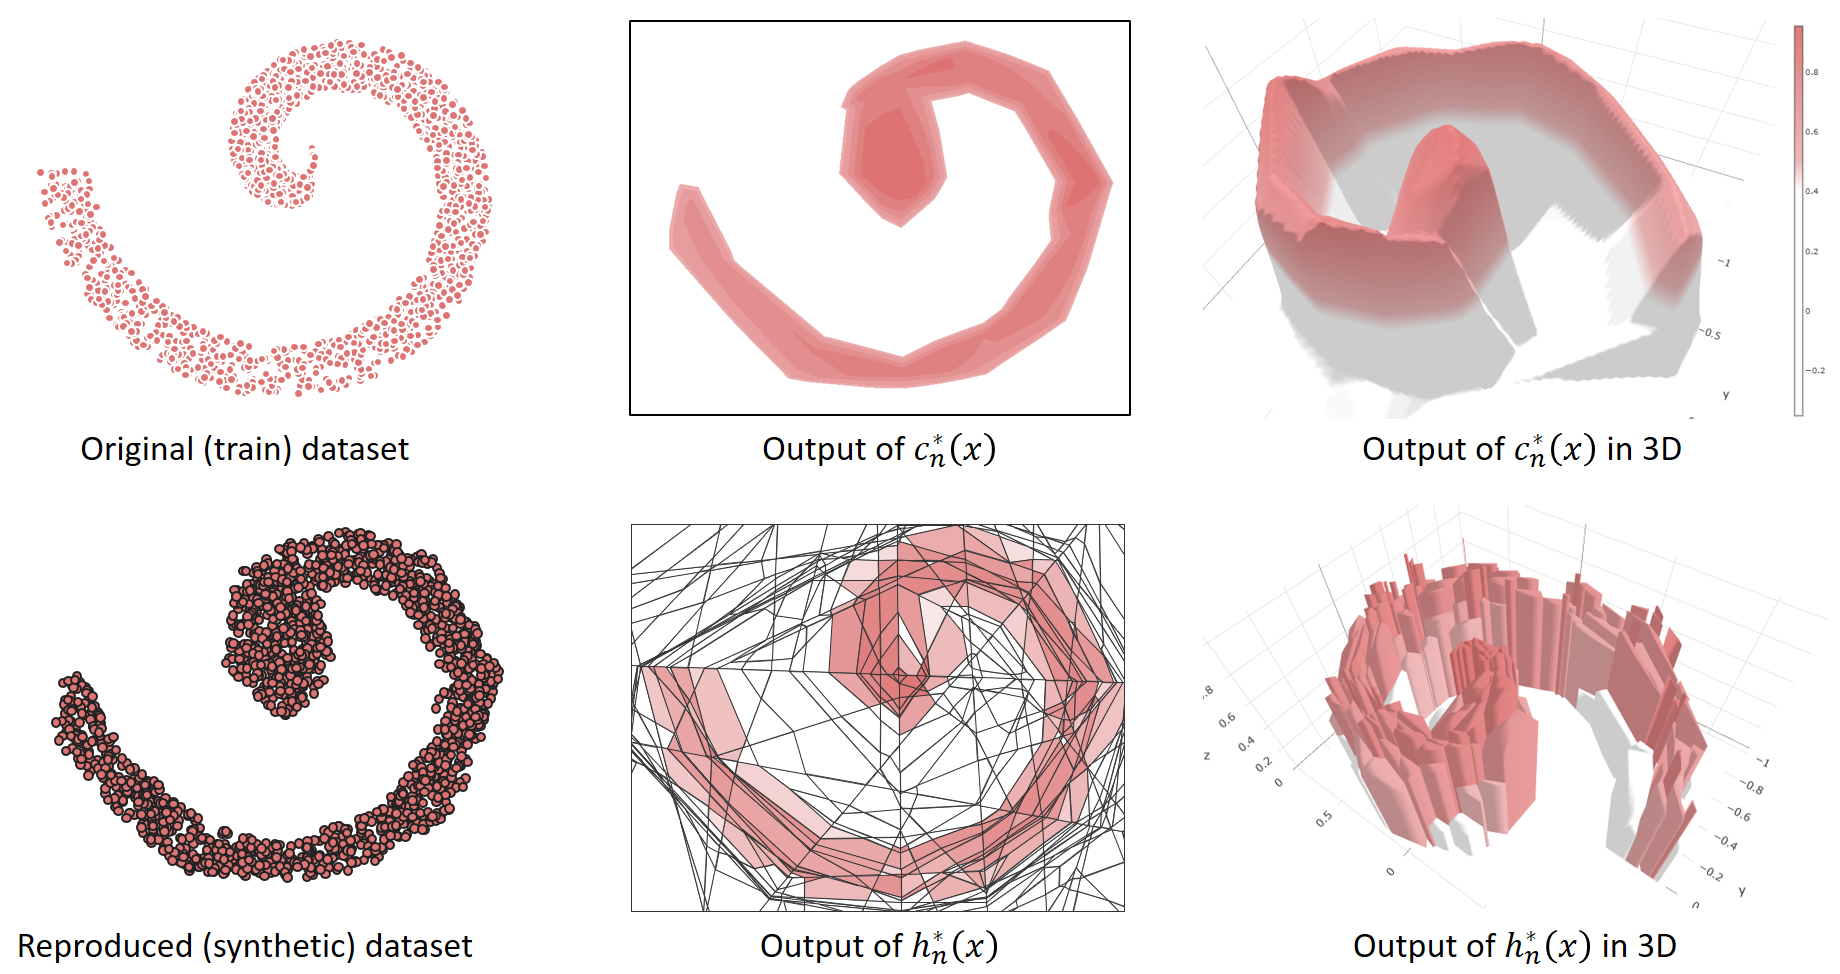
\includegraphics[width=0.32\linewidth]{Dissertation/images/ch3/reproduction/spiral.png}}
        \hfill
        \subcaptionbox{Два квадрата}{%
            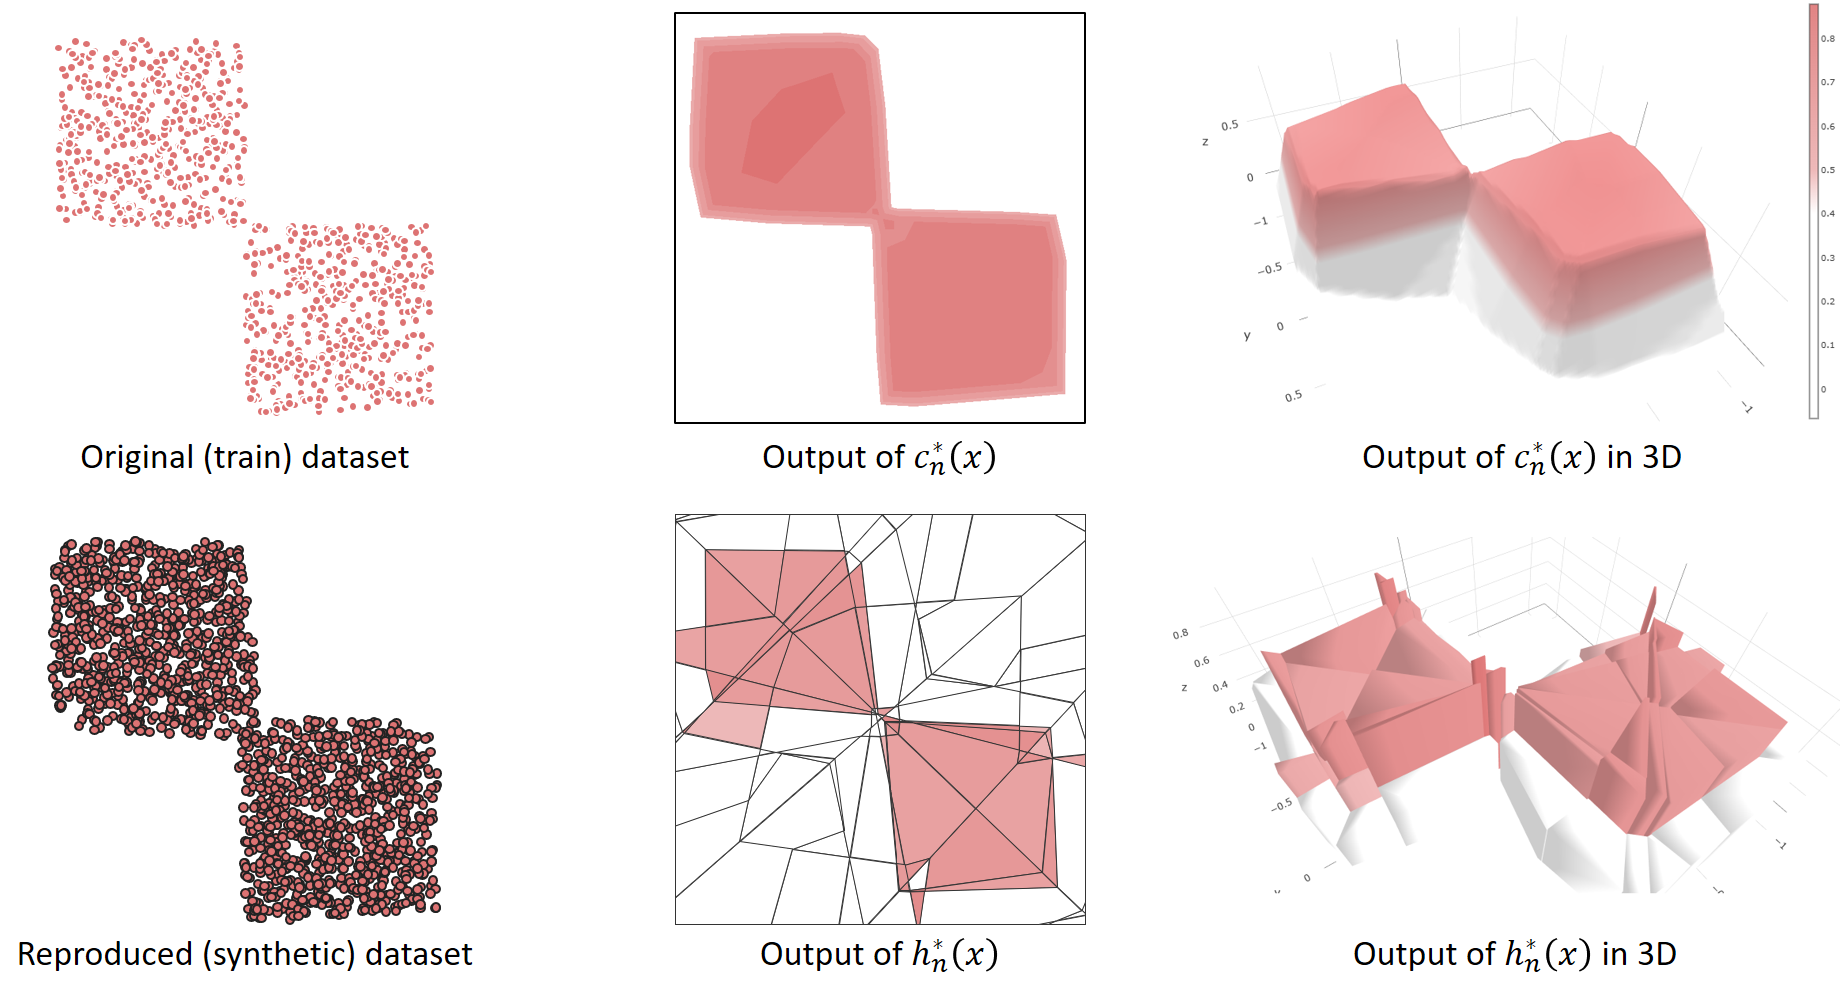
\includegraphics[width=0.32\linewidth]{Dissertation/images/ch3/reproduction/two-square.png}}
        \hfill
        \subcaptionbox{Смесь нормальных распределений}{%
            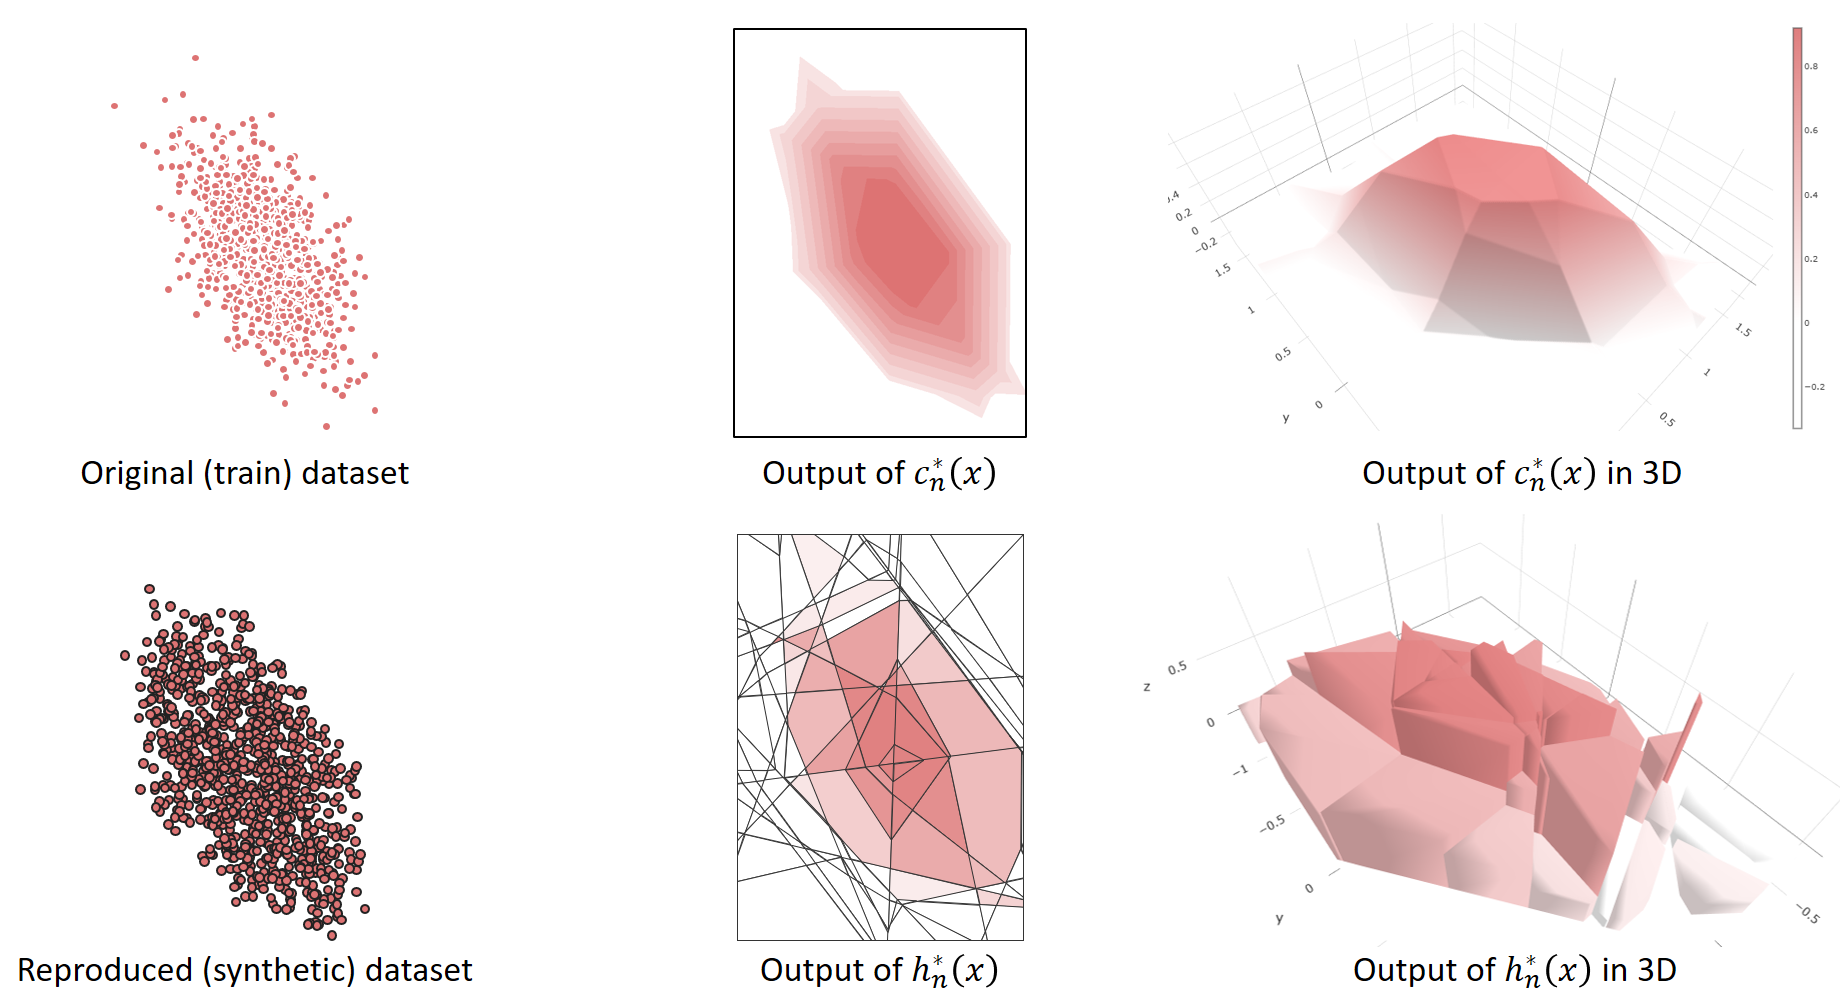
\includegraphics[width=0.32\linewidth]{Dissertation/images/ch3/reproduction/gaussian.png}}
        \hfill
    }
    \caption{результаты эксперимента с синтетическими данными}
    \label{fig:synthetic_results}
\end{figure}

\subsubsection{Архитектура и параметры обучения}

Модель обучалась на 100 эпохах, размер батча -- 32. Использовались различные архитектуры сети:
\begin{itemize}
  \item \textbf{d-10-1}: минималистичная модель с одним скрытым слоем.
  \item \textbf{d-10-100-1}: глубокая архитектура с повышенной ёмкостью.
  \item \textbf{d-10-10-10-1}: сбалансированная конфигурация.
\end{itemize}

Оптимизация осуществлялась методом Adam~\cite{adam2014method} с шагом обучения \(10^{-3}\). Функция активации -- модульная.

\subsubsection{Ограничения}

Преимущество предложенного подхода заключается в естественной аппроксимации плотности через сетевую структуру, эквивалентную адаптивной гистограмме. Однако с ростом размерности пространства наблюдается ухудшение качества генерации из-за разреженности, что требует более сложной архитектуры и дополнительных механизмов фильтрации. Одним из решений является введение более высокого порога уверенности \(\beta\), при котором в синтетическую выборку включаются только точки с \(c(x) > \beta\), снижая шум, но уменьшая разнообразие.

Кроме того, в отличие от генеративных моделей, основанных на латентных переменных (например, CTGAN \cite{habibi2023imbalanced}, TVAE \cite{ishfaq2018tvae}), рассматриваемый метод не требует обучения скрытого представления и обладает более прозрачной интерпретируемостью за счёт прямой связи с оценкой плотности.

Важно отметить, что модель может наследовать структурные и социальные смещения из обучающих данных. Поэтому при генерации синтетических выборок, особенно в задачах с социально значимой информацией, требуется дополнительный контроль справедливости.

\subsubsection{Выводы}

Таким образом, метод построения репродукционных выборок через унарную классификацию представляет собой эффективную альтернативу генеративным моделям. Он сочетает в себе простоту реализации, теоретическую интерпретируемость и способность воспроизводить сложные структуры данных. Это делает его перспективным инструментом для синтетической генерации данных, особенно в условиях ограниченного доступа к реальным выборкам.

\section{Обучение нейросети по некомплектным данным}

Отсутствие значений в данных (\emph{пропуски}) представляет собой одну из наиболее распространённых и при этом наименее формализованных проблем, с которой сталкиваются в прикладном машинном обучении и статистическом анализе. Согласно \cite{little1995statistical}, в любой области, где данные собираются при помощи опросов, сенсоров или в рамках наблюдательных исследований, практически неизбежно возникает неполнота -- отсутствие значений некоторых признаков у части объектов выборки. Такая ситуация наблюдается в биомедицинских данных~\cite{cismondi2013missing}, социологических опросах, прикладных инженерных задачах, финансовом моделировании и других областях.

Пропуски могут быть обусловлены множеством факторов: техническими сбоями~\cite{du2020missing}, отказами респондентов отвечать на конкретные вопросы, ограничениями ресурсоёмких измерений, фильтрацией данных, нарушениями сбора и хранения. При этом даже небольшое число пропущенных значений может существенно повлиять на результаты анализа, особенно при высокой размерности признакового пространства или в задачах, чувствительных к структуре выборки.

Корректное обращение с пропущенными значениями требует не только выбора соответствующей стратегии заполнения, но и понимания механизма возникновения пропусков. Как подчёркивается в \cite{little1995statistical, schafer1997analysis}, пренебрежение механизмом отсутствия может привести к систематическим ошибкам, смещению оценок, снижению статистической мощности и искажению выводов. Особенно это критично в задачах обучения нейросетей, где входные данные передаются в модели в виде числовых векторов, не допускающих наличия неопределённых компонент.

\subsection{Задача классификации данных с пропущенными значениями}

Пусть имеется обучающая выборка из \(n\) объектов: \( \{(X_i, Y_i)\}_{i=1}^n \), где \(X_i \in [0, 1]^d\) -- вектор признаков, а \(Y_i \in \{1, 2, \dots, C\}\) -- метка класса. Предполагается, что некоторые признаки могут быть пропущены. Для описания структуры отсутствующих данных вводится матрица \(M \in \{0, 1\}^{n \times d}\), где \(m_{ij} = 1\) означает, что признак \(j\) отсутствует у объекта \(i\), а \(m_{ij} = 0\) -- признак наблюдаем.

Обозначим через \(X_0\) множество наблюдаемых признаков, а через \(X_1\) -- множество отсутствующих.

\subsection{Типы механизмов пропусков}

Следуя формализации, приведённой в \cite{little1995statistical}, различают три основных типа пропусков:

\begin{itemize}
    \item Пропуски, отсутствующие полностью случайно (MCAR, missing completely at random): механизм пропусков не зависит ни от наблюдаемых, ни от ненаблюдаемых данных. Формально, \(P(M \mid X_0, X_1, Y) = P(M)\).
    \item Пропуски, отсутствующие случайно (MAR, missing at random): вероятность отсутствия значения может зависеть от наблюдаемых данных, но не от пропущенных. То есть \(P(M \mid X_0, X_1, Y) = P(M \mid X_0, Y)\).
    \item Пропуски, отсутствующие не случайно (NMAR, not missing at random): вероятность отсутствия значения зависит от ненаблюдаемых данных, т.е. \(P(M \mid X_0, X_1, Y)\) не сводится к предыдущим случаям.
\end{itemize}

При предположении MCAR и MAR допускается игнорирование механизма пропусков при построении модели. В случае NMAR необходимо явно моделировать процесс отсутствия данных, что усложняет задачу.

\subsection{Существующие методы обработки пропусков}

В литературе представлены различные стратегии, позволяющие бороться с неполнотой данных. Кратко охарактеризуем наиболее известные из них.

\subsubsection{Удаление некомплектных наблюдений}

Простейший метод -- исключение строк с пропущенными значениями. Такой подход корректен только при MCAR и при условии, что доля удаляемых объектов незначительна. Основной недостаток -- потеря потенциально полезной информации и возможное смещение выборки.

\subsubsection{Заполнение средним значением (mean imputation)}

Отсутствующие значения заменяются средним по соответствующему признаку, вычисленным по доступным наблюдениям:
\[
x_{ij} \leftarrow \frac{1}{|\mathcal{I}_j|} \sum_{i \in \mathcal{I}_j} x_{ij}, \quad \mathcal{I}_j = \{ i \mid m_{ij} = 0 \}.
\]
Метод не учитывает зависимость между признаками, занижает дисперсию и нарушает ковариационную структуру данных.

\subsubsection{Заполнение медианой или модой}

Применяется для категориальных признаков (мода) или числовых с выбросами (медиана). Устраняет чувствительность к экстремальным значениям, но по-прежнему игнорирует корреляции и структуру признаков.

\subsubsection{\(k\)-ближайших соседей (kNN imputation)}

Для объекта с пропущенным признаком ищется множество \(k\) ближайших (по наблюдаемым координатам) объектов, и пропущенное значение заполняется агрегатом (среднее, медиана) по этому множеству. Обозначим через \( \mathcal{N}_k(i) \) множество \(k\)-соседей объекта \(i\). Тогда:
\[
x_{ij} \leftarrow \frac{1}{k} \sum_{\ell \in \mathcal{N}_k(i)} x_{\ell j}.
\]
Метод чувствителен к выбору метрики, неустойчив при высокой разреженности и требует полного набора значений для вычисления расстояний~\cite{pujianto2019k}.

\subsubsection{Множественное заполнение и EM-алгоритм}

В рамках подхода максимального правдоподобия в \cite{dempster1977maximum} вводится вероятностная модель данных и итеративно оцениваются параметры и пропущенные значения. На шаге \textbf{E} оценивается распределение некомплектных данных при фиксированных параметрах, на шаге \textbf{M} -- параметры по комплектным данным. Подход требует априорных предположений о распределении данных (обычно гауссовское) и высоких вычислительных затрат. В случае множественного заполнения \cite{rubin1988overview} создаётся несколько возможных вариантов с последующей агрегацией.

\subsubsection{Методы на основе PCA и автокодировщиков}

Пропуски заполняются с помощью аппроксимации данных в латентном пространстве. В методах PCA недостающие значения восстанавливаются проекцией на подпространство главных компонент~\cite{moh2024missing}. В нейросетевом варианте -- автокодировщики обучаются на комплектных данных и используются для реконструкции пропущенных~\cite{roskams2023leveraging}.

\subsection{Ограничения классических методов}

Все перечисленные методы обладают рядом общих недостатков:
\begin{itemize}
    \item не учитывают апостериорную неопределённость заполнения;
    \item вводят систематическое смещение в оценки параметров модели;
    \item теряют вариативность по заполненным признакам;
    \item игнорируют структуру задачи (например, наличие классов в классификации).
\end{itemize}

Таким образом, возникает необходимость в методах, которые позволяли бы обрабатывать некомлпектные данные без грубых аппроксимаций, использовали бы информацию о метках классов и сохраняли бы стохастический характер восстановления недостающих признаков.

В работе~\cite{perminov2025missing} предлагается альтернативный метод, основанный на вероятностном заполнении признаков с помощью унарной классификации и многослойного персептрона.

\subsection{Метод вероятностного заполнения}

Пусть \(X \in [0, 1]^{n \times d}\) -- обучающая выборка с пропущенными значениями, \(Y \in \{0, 1, \dots, C\}^n\) -- вектор меток классов, \(M \in \{0, 1\}^{n \times d}\) -- матрица пропусков. Предполагается, что механизм пропусков является случайным (MCAR или MAR по классификации Рубина~\cite{little1995statistical}).

Предлагаемый метод обучения MLP при наличии пропусков в обучающей выборке применяется последовательно к каждому из \(C\) классов и состоит из трёх шагов (схематичное изображение методики изображено на рисунке~\cref{fig:missing_diagram}):

\begin{enumerate}

    \item \textbf{Начальное обучение.} Для комплектной подвыборки \(\{X\}_i^n\) \(j\)-го класса, \(j \in \{1, 2, \cdots C\}\), решить задачу унарной классификации и построить персептрон, реализующий кусочно-линейную непрерывную функцию \(c_n^{(j)}(X)\).
    
    \item \textbf{Дообучение.} Дообучение  осуществляется по всей обучающей выборке \(j\)-го класса отдельными эпохами. Перед текущей эпохой выполнить временное (для данной эпохи) заполнение некомплектных наблюдений. Для каждого некомплектного наблюдения \(X\):

    \begin{enumerate}
        \item Разделить множество индексов координат вектора \(X=(x_1, x_2, \cdots, x_d)\) на два подмножества \(M_0\) и \(M_1\), включающие соответственно индексы заполненных и пропущенных координат. 
        
        \item Заполнить координаты \(X\) из \(M_1\) наблюдениями равномерно распределенной случайной величины на отрезке \([0, 1]\), в результате чего будет получен комплектный вектор \(X'\). Вычислить \(c_n^{(j)}(X')\). Сгенерировать наблюдение биномиальной случайной величины с вероятностью успеха \(p=c_n^{(j)}(X')\).
        
        \item При успешном исходе временно заменить в обучающей выборке некомплектный вектор \(X\) на комплектный вектор \(X'\) и перейти к рассмотрению следующего некомплектного наблюдения. В противном случае повторить предыдущий шаг.
        
        \item Выполнить дообучение сети по ``доукомплектованной`` обучающей выборке.
    \end{enumerate}
    
    \item Перейти к следующей эпохе дообучения, повторяя шаги а-г, до полного завершения обучения \(MLP_j\) для \(j\)-го класса с функцией нейросетевой регрессии \(c_n^{(j)}(X)\).
\end{enumerate}

Повторяя шаги 1-3 для всех классов, получим \(C\) обученных нейросетей \(MLP_j\) и соответствующих им непрерывных кусочно-линейных функций \(\{c_n^{(1)}(X), c_n^{(2)}(X), \cdots, c_n^{(C)}(X)\}\), каждая из которых есть выборочная оценка апостериорной вероятности соответствующего класса в точке \(X\).

\begin{figure}[ht]
    \centerfloat{
        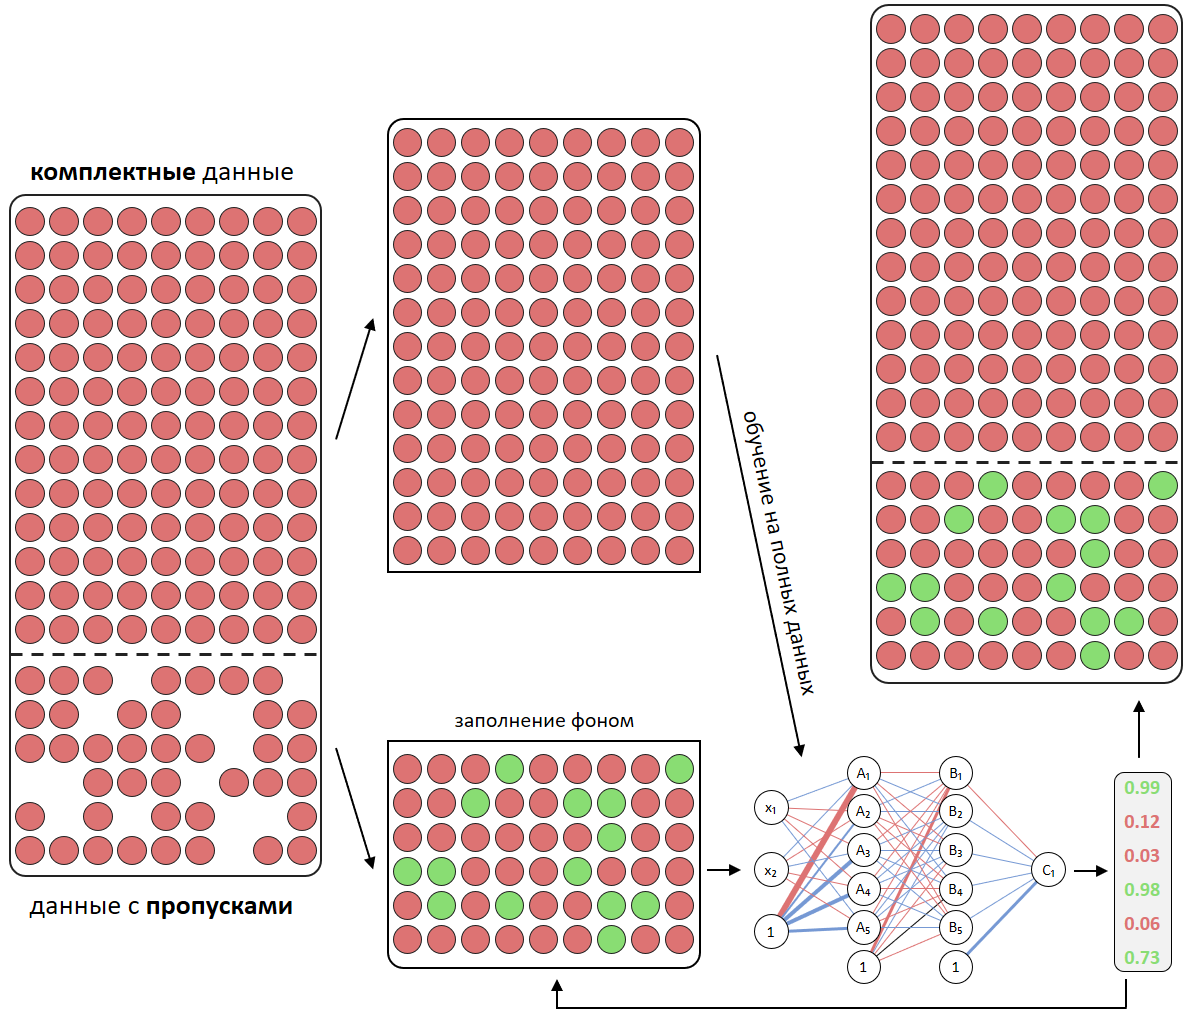
\includegraphics[width=\linewidth]{Dissertation/images/ch3/missing_data/diagram.png}
    }
    \caption{Схема обучения \(c_n^{(j)}(X)\) по некомплектным данным}
    \label{fig:missing_diagram}
\end{figure}


\subsection{Классификация комплектного наблюдения}

Для решения задачи классификации комплектного наблюдения \(X\) возможны различные стратегии. Простейшая состоит в выборе класса, для которого апостериорная вероятность максимальна. Другой вариант -- выбрать в качестве решения все классы, значения апостериорной вероятности для которых больше некоторого заданного порога, и продолжить решение задачи классификации, например, в другом признаковом пространстве.

\subsection{Экспериментальное исследование}

Для экспериментального анализа были подготовлены несколько модельных наборов данных с чёткой визуальной и статистической интерпретацией классов. Это позволило обеспечить контролируемую среду и надёжную оценку устойчивости моделей к пропущенным значениям.

\subsubsection{Используемые наборы данных}
\begin{itemize}
    \item \textbf{Гауссианы} -- два нормально распределённых кластера с равной дисперсией и небольшим перекрытием (рисунок~\cref{fig:missed_datasets}\subcaptionref{fig:missed_datasets_gaussians}).
    \item \textbf{Спирали} -- классы формируют витки спиралей с общей точкой начала координат, разделение классов сильно нелинейное (рисунок~\cref{fig:missed_datasets}\subcaptionref{fig:missed_datasets_spiral}).
    \item \textbf{Кольцо и круг} -- один класс расположен внутри круга, второй образует кольцо с зазором между границами (рисунок~\cref{fig:missed_datasets}\subcaptionref{fig:missed_datasets_circle}).
\end{itemize}

\begin{figure}[ht]
    \centerfloat{
        \hfill
        \subcaptionbox{Гауссианы\label{fig:missed_datasets_gaussians}}{%
            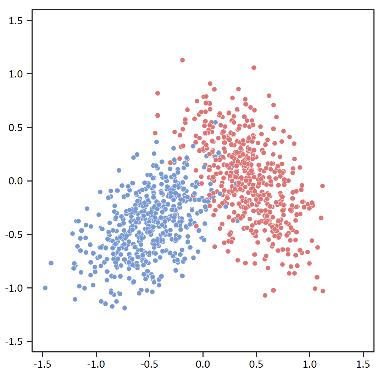
\includegraphics[width=0.32\linewidth]{Dissertation/images/ch3/missing_data/gaussians.png}}
        \hfill
        \subcaptionbox{Спираль\label{fig:missed_datasets_spiral}}{%
            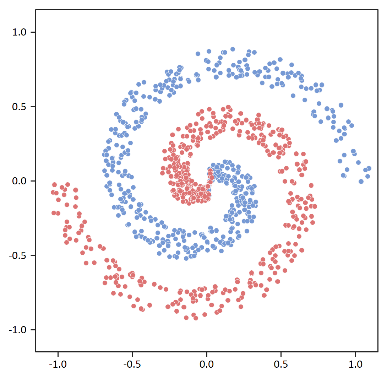
\includegraphics[width=0.32\linewidth]{Dissertation/images/ch3/missing_data/spirals.png}}
        \hfill
        \subcaptionbox{Кольцо и круг\label{fig:missed_datasets_circle}}{%
            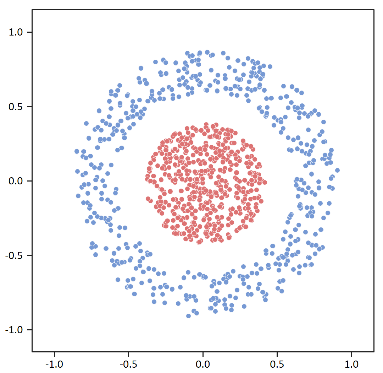
\includegraphics[width=0.32\linewidth]{Dissertation/images/ch3/missing_data/circles.png}}
        \hfill
    }
    \caption{Использованные наборы для обучения модели на данных с пропусками}
    \label{fig:missed_datasets}
\end{figure}

\subsubsection{Обработка пропущенных значений}
Во всех наборах данных искусственно вводились пропуски в признаках с уровнями 20\%, 40\%, 50\%, 60\%, 80\% и 90\%. Пропуски вносились случайно и только в признаках (целевые метки всегда сохранялись). Были рассмотрены следующие классические методы обработки пропусков:

\begin{itemize}
    \item \textbf{mean} -- заполнение по среднему значению признака;
    \item \textbf{mode} -- заполнение наиболее частым значением;
    \item \textbf{\(kNN (k=3)\)} -- заполнение по ближайшим трём соседям в евклидовом пространстве;
    \item \textbf{\(kNN (k=7)\)} -- аналогично, но с \(k=7\);
    \item \textbf{reproduction} (предложенный метод) -- метод, основанный на унарной классификации.
\end{itemize}

\subsubsection{Сценарии обучения}
Для каждой комбинации набора данных и уровня пропусков модель обучалась в следующих режимах:

\begin{itemize}
    \item \textbf{full} -- обучение на полном наборе без пропусков;
    \item \textbf{complete} -- обучение только на тех примерах, где отсутствуют пропуски;
    \item \textbf{imputed} -- обучение на наборе, где пропуски заполнялись одним из методов.
\end{itemize}

В качестве модели использовался многослойный персептрон с \(L=2\) скрытыми слоями по \(k=20\) нейронов в каждом и одним выходным слоем. Обучение осуществлялось на протяжении 500 эпох.

Каждая комбинация набора данных, уровня пропусков и метода заполнения запускалась 50 раз с различными начальными инициализациями весовых коэффициентов. В качестве основной метрики использовалась точность классификации (accuracy) на тестовом множестве из соответствующего набора данных из 5000 элементов. Все тестовые наборы содержали только комплектные данные.

Для метода репродукции персептрон обучался в течение 50 эпох на данных без пропусков, а затем каждую эпоху запускался процесс вероятностного заполнения пропусков и обучение продолжалось уже на обновлённых заполненных данных.

\subsubsection{Результаты}
Сводные таблицы \cref{tab:missing_results_gaussians}, \cref{tab:missing_results_spiral} и \cref{tab:missing_results_circle} по accuracy (в среднем по 50 запускам) представлены ниже. Визуальный анализ показывает, что метод репродукции демонстрирует более высокую устойчивость при высоких уровнях пропусков, особенно на сложных наборах данных, как например "кольцо и круг". Традиционные методы заполнения (среднее, мода) показывают ожидаемое снижение качества, особенно при пропусках выше 60\%. Метод \(kNN\) даёт умеренное улучшение, но чувствителен к плотности выборки.

\begin{table} [htbp]
    \centering
    \begin{threeparttable}
        \caption{Оценка метода репродукции для заполнения пропусков на наборе данных ``Гауссианы``}\label{tab:missing_results_gaussians}
        \begin{SingleSpace}
        \begin{tabular}{|c|c|c|c|c|c|}
            \hline
            Доля & full & complete & reproduce & mean & knn 7 \\
            \hline
            20\% &       & 0.919±0.006 & \textbf{0.925±0.004} & 0.917±0.007 & 0.921±0.006 \\
            40\% &       & \textbf{0.919±0.006} & 0.917±0.009 & 0.897±0.008 & 0.915±0.005 \\
            50\% & 0.925 & 0.917±0.005 & \textbf{0.918±0.008} & 0.904±0.014 & 0.917±0.005 \\
            60\% &   ±   & 0.910±0.013 & \textbf{0.921±0.009} & 0.866±0.018 & 0.894±0.012 \\
            80\% & 0.003 & 0.875±0.011 & \textbf{0.912±0.008} & 0.752±0.047 & 0.851±0.011 \\
            90\% &       & 0.842±0.023 & \textbf{0.906±0.007} & 0.593±0.092 & 0.806±0.015 \\
            \hline
        \end{tabular}
        \end{SingleSpace}
    \end{threeparttable}
\end{table}


\begin{table} [htbp]
    \centering
    \begin{threeparttable}
        \caption{Оценка метода репродукции для заполнения пропусков на наборе данных ``Спираль``}\label{tab:missing_results_spiral}
        \begin{SingleSpace}
        \begin{tabular}{|c|c|c|c|c|c|}
            \hline
            Доля & full & complete & reproduce & mean & knn 7 \\
            \hline
            20\% &       & 0.936±0.031 & \textbf{0.945±0.025} & 0.922±0.032 & 0.941±0.020 \\
            40\% &       & 0.924±0.023 & \textbf{0.930±0.021} & 0.899±0.034 & 0.918±0.025 \\
            50\% & 0.941 & \textbf{0.926±0.016} & 0.910±0.034 & 0.893±0.031 & 0.868±0.062 \\
            60\% &   ±   & \textbf{0.913±0.030} & 0.898±0.047 & 0.890±0.027 & 0.853±0.040 \\
            80\% & 0.024 & \textbf{0.869±0.039} & 0.861±0.044 & 0.750±0.095 & 0.773±0.062 \\
            90\% &       & \textbf{0.827±0.042} & 0.812±0.067 & 0.545±0.082 & 0.695±0.040 \\
            \hline
        \end{tabular}
        \end{SingleSpace}
    \end{threeparttable}
\end{table}

\begin{table} [htbp]
    \centering
    \begin{threeparttable}
        \caption{Оценка метода репродукции для заполнения пропусков на наборе данных ``Кольцо и круг``}\label{tab:missing_results_circle}
        \begin{SingleSpace}
        \begin{tabular}{|c|c|c|c|c|c|}
            \hline
            Доля & full & complete & reproduce & mean & knn 7 \\
            \hline
            20\% &       & 0.987±0.009 & \textbf{0.989±0.006} & 0.941±0.058 & 0.927±0.086 \\
            40\% &       & 0.984±0.011 & \textbf{0.986±0.011} & 0.865±0.103 & 0.846±0.123 \\
            50\% & 0.981 & 0.971±0.019 & \textbf{0.984±0.016} & 0.852±0.094 & 0.751±0.149 \\
            60\% &   ±   & 0.974±0.018 & \textbf{0.981±0.016} & 0.763±0.083 & 0.705±0.103 \\
            80\% & 0.014 & 0.892±0.136 & \textbf{0.964±0.031} & 0.609±0.148 & 0.618±0.069 \\
            90\% &       & 0.852±0.080 & \textbf{0.952±0.038} & 0.295±0.126 & 0.562±0.055 \\
            \hline
        \end{tabular}
        \end{SingleSpace}
    \end{threeparttable}
\end{table}
           % Глава 3
\chapter{Интеллектуальная система машинного обучения для визуализации и исследования методов классификации}

\section{Общая характеристика интеллектуальной системы машинного обучения}

В рамках выполненного исследования была разработана интеллектуальная система машинного обучения, предназначенная для визуального и экспериментального изучения поведения моделей классификации в условиях ограниченного объёма обучающих данных, дисбаланса классов, а также в присутствии фона и пропущенных значений. Система представляет собой автономное клиентское приложение, реализованное на языке JavaScript~\cite{flanagan2013javascript}, не требующее установки, интернет-соединения или использования графического ускорителя, что обеспечивает его широкую доступность и воспроизводимость экспериментов.

Интеллектуальная система предназначена для комплексной демонстрации, отладки и тестирования алгоритмов, описанных в теоретических разделах настоящей работы. Предоставляется интуитивно понятный графический интерфейс с возможностью гибкой настройки параметров моделей, наборов данных и условий обучения. Благодаря использованию визуальных компонентов пользователь может в интерактивном режиме наблюдать за процессом формирования разделяющих поверхностей, анализировать выходы моделей, а также проводить тестирование устойчивости классификаторов.

Разработка велась с учётом необходимости масштабируемости архитектуры: структура системы разделена на независимые функциональные блоки, что обеспечивает возможность расширения и модификации без необходимости переписывания всего кода. Интерфейс системы логически организован по вкладкам, каждая из которых отвечает за определённую группу задач: генерация и загрузка данных, обучение модели, проведение экспериментов, визуализация и анализ результатов.

На момент завершения работы интеллектуальная система машинного обучения включает в себя следующие ключевые функциональные возможности:
\begin{itemize}
    \item настройка параметров архитектуры многослойного персептрона, включая размеры и количество слоёв, выбор функции активации, установку порогов доверия;
    \item управление параметрами обучения (функция потерь, оптимизатор, регуляризация, и т.д.);
    \item пошаговая визуализация процесса обучения, включая изменение выходов модели, метрик и формирование ячеек;
    \item реализация как классических методов бинарной классификации, так и модифицированного метода с фоном;
    \item визуализация, построение и загрузка обучающих и тестовых множеств;
    \item проведение экспериментальных исследований по созданию синтетических данных, обработке данных с пропусками, а также анализ объясняющего двоичного дерева eXBTree.
\end{itemize}

Таким образом, система реализует весь цикл исследования: от генерации обучающего множества до визуализации результатов и анализа поведения модели в различных условиях. Её применение позволяет не только демонстрировать основные методы, описанные в главах 1–3, но и проводить дополнительный количественный и качественный анализ, направленный на верификацию теоретических положений.

\section{Архитектура и интерфейс интеллектуальной системы}

Разработанная система реализована на JavaScript с использованием стандартных веб-технологий: HTML5~\cite{hickson2011html5}, CSS3~\cite{lunn2012css3}, SVG~\cite{quint2003scalable} и Canvas API~\cite{lubbers2010using}. Для стилизации применяется собственный CSS без привлечения сторонних фреймворков. Взаимодействие между компонентами построено на событийной модели с использованием собственного класса-эмиттера событий (EventEmitter). Основным управляющим объектом является класс Playground, который инкапсулирует логику координации работы всех компонентов и обмена данными между ними. Все вычисления производятся на стороне клиента, что исключает необходимость обращения к внешним серверам и обеспечивает полную автономность работы.

%%%%%%%%%%%%%%%%%%%%%%%%%%%%%%%%%%%%%%%%%%%%%%%%%%%%%%%%%%%%%%%%%%%%%%%%%%%%%%%%%%%%%%%%%%%%%%%%%%%%%%%%%%%%%%%
\subsection{Архитектура интеллектуальной системы}

Архитектура системы выполнена по модульному принципу, включая следующие ключевые блоки:

\begin{itemize}
    \item \textbf{Модуль данных} -- отвечает за генерацию, хранение и загрузку обучающих и тестовых наборов.
    \item \textbf{Модуль модели} -- реализует обучение персептрона и его использование для анализа.
    \item \textbf{Модуль обучения} -- реализует методы градиентного спуска, алгоритмы оптимизации и функций потерь, а также формирование модифицированных обучающих выборок с фоновым распределением.
    \item \textbf{Модуль визуализации} -- занимается отрисовкой данных, иерархии ячеек, карты предсказаний, структурных элементов модели, а также графиков метрик и гистограмм. Визуализация осуществляется с помощью Canvas API и SVG.
    \item \textbf{Модуль экспериментов} -- обеспечивает выполнение преднастроенных экспериментов, таких как анализ дерева eXBTree, создание синтетических данных и обучение модели на данных с пропусками.
    \item \textbf{Модуль управления} -- реализует пользовательский интерфейс, включая меню, формы настройки параметров и кнопки управления, а также обработку событий от пользователя.
\end{itemize}

Все модули взаимодействуют между собой через механизм событий, что обеспечивает слабую связанность и гибкость расширения. Класс Playground выступает центральным контроллером, инициализирующим компоненты, регистрирующим слушатели событий и передающим данные между модулями.

%%%%%%%%%%%%%%%%%%%%%%%%%%%%%%%%%%%%%%%%%%%%%%%%%%%%%%%%%%%%%%%%%%%%%%%%%%%%%%%%%%%%%%%%%%%%%%%%%%%%%%%%%%%%%%%
\subsection{Структура интерфейса}

Интерфейс интеллектуальной системы структурирован по трём основным вкладкам, каждая из которых реализована как независимый набор компонентов с собственным меню и областью отображения:

\begin{itemize}
    \item \textbf{Вкладка ``Данные``} -- предоставляет средства генерации и файловой загрузки наборов данных. Отображение данных осуществляется в табличном виде и на графике с цветовой кодировкой для обучающего и тестового разбиений. Имеются инструменты нормализации и экспорта данных.

    \item \textbf{Вкладка ``Обучение``} -- главный визуально насыщенный раздел, где происходит настройка архитектуры модели (число слоёв, размер слоёв, функции активации, порог доверия), параметров обучения (скорость, функция потерь, оптимизатор, регуляризация) и параметров визуализации (отображение выходов модели и формируемых ячеек, точки обучающего, тестового и фонового множеств). Обучение может как запускаться и останавливаться по желанию, так и выполняться в виде единственного шага. Область просмотра динамически отображает состояние модели, метрики и распределение выходов персептрона на обучающих данных в виде гистограмм.

    \item \textbf{Вкладка ``Эксперименты``} -- содержит инструменты для запуска и анализа различных сценариев: анализ двоичного объясняющего дерева, создание синтетических данных, а также обучение модели на данных с пропусками. Результаты представлены в виде интерактивных таблиц, графиков и гистограмм, позволяющих детально исследовать поведение модели.
\end{itemize}

Интерфейс спроектирован с акцентом на интерактивность и прозрачность процесса: изменение параметров мгновенно отражается на визуализации, что позволяет пользователю оперативно оценивать влияние настроек.

%%%%%%%%%%%%%%%%%%%%%%%%%%%%%%%%%%%%%%%%%%%%%%%%%%%%%%%%%%%%%%%%%%%%%%%%%%%%%%%%%%%%%%%%%%%%%%%%%%%%%%%%%%%%%%%
\subsection{Аппаратные и программные требования}

Интеллектуальная система машинного обучения не требует установки дополнительных библиотек или серверной инфраструктуры. Для работы необходим любой современный браузер с поддержкой Javascript, HTML5 Canvas и SVG. Ресурсоёмкость минимальна, что позволяет запускать систему на большинстве персональных компьютеров без специальных требований.

\section{Реализованные алгоритмы и методы визуализации}

В интеллектуальной системе реализован широкий спектр алгоритмов и методов, необходимых для обучения, визуализации и анализа моделей нейросетевой классификации, а также для работы с неполными и синтетическими данными. Приведённые ниже компоненты составляют ядро вычислительного и аналитического функционала системы.

%%%%%%%%%%%%%%%%%%%%%%%%%%%%%%%%%%%%%%%%%%%%%%%%%%%%%%%%%%%%%%%%%%%%%%%%%%%%%%%%%%%%%%%%%%%%%%%%%%%%%%%%%%%%%%%
\subsection{Многослойный персептрон}
В качестве основной вычислительной модели реализован многослойный персептрон, представленный в виде набора последовательно соединённых полносвязных слоёв. Каждый слой выполняет матрично-векторное преобразование входных признаков с последующим применением нелинейной активации. Архитектура поддерживает произвольную глубину и размерность слоёв, задаваемую пользователем.

Особое внимание уделено производительности реализации. В целях обеспечения вычислительной эффективности произведено разворачивание вложенных циклов~\cite{huang1999generalized} и оптимизация операций умножения с использованием предварительного выделения буферов. Все операции реализованы в терминах низкоуровневых операций над типизированными массивами~\cite{matsakis2014typed} JavaScript, без применения сторонних библиотек.

%%%%%%%%%%%%%%%%%%%%%%%%%%%%%%%%%%%%%%%%%%%%%%%%%%%%%%%%%%%%%%%%%%%%%%%%%%%%%%%%%%%%%%%%%%%%%%%%%%%%%%%%%%%%%%%
\subsection{Оптимизационные алгоритмы}
Для обучения нейросетевых моделей реализованы различные варианты стохастического градиентного спуска:

\begin{itemize}
    \item SGD -- базовый метод без накопления импульса;
    \item SGD с импульсом (momentum) -- учитывает направление предыдущих градиентов;
    \item Adam -- использует адаптивную нормализацию градиентов на основе скользящих средних;
    \item Adamax, Adagrad, RMSprop, Adadelta~\cite{zeiler2012adadelta} — альтернативные адаптивные модификации~\cite{ruder2016overview}, отличающиеся способами обновления весов.
\end{itemize}

Каждый из алгоритмов может быть выбран пользователем, параметры (скорость обучения, размер пакета) доступны для настройки в пользовательском интерфейсе.

%%%%%%%%%%%%%%%%%%%%%%%%%%%%%%%%%%%%%%%%%%%%%%%%%%%%%%%%%%%%%%%%%%%%%%%%%%%%%%%%%%%%%%%%%%%%%%%%%%%%%%%%%%%%%%%
\subsection{Функции потерь}
Система поддерживает несколько типов функций потерь, применяемых как для задач классификации, так и регрессии:

\begin{itemize}
    \item Среднеквадратичная ошибка (MSE);
    \item Средняя абсолютная ошибка (MAE);
    \item Потеря Хубера~\cite{meyer2021alternative} (Huber loss);
    \item Логарифмическая гиперболическая косинус-функция~\cite{saleh2022statistical} (Log-Cosh).
\end{itemize}

Функции потерь реализованы вручную, с учётом числовой устойчивости и эффективности вычислений.

%%%%%%%%%%%%%%%%%%%%%%%%%%%%%%%%%%%%%%%%%%%%%%%%%%%%%%%%%%%%%%%%%%%%%%%%%%%%%%%%%%%%%%%%%%%%%%%%%%%%%%%%%%%%%%%
\subsection{Объясняющее двоичное дерево}
Для анализа принятия решений реализован алгоритм построения объясняющего двоичного дерева. Дерево формируется по реальным выходам модели на имеющихся данных, без рассмотрения всех гипотетических состояний пространства (что позволяет избежать экспоненциального роста сложности). Структура дерева отображается в виде таблицы ячеек, с указанием статистических характеристик.

%%%%%%%%%%%%%%%%%%%%%%%%%%%%%%%%%%%%%%%%%%%%%%%%%%%%%%%%%%%%%%%%%%%%%%%%%%%%%%%%%%%%%%%%%%%%%%%%%%%%%%%%%%%%%%%
\subsection{Визуализация модели и метрик}
Визуализация является ключевой частью интеллектуальной системы машинного обучения. Реализованы следующие возможности:

\begin{itemize}
    \item Построение выходной поверхности модели (в двумерном или трёхмерном виде) с применением различных цветовых схем (рисунок~\cref{fig:vis_model_output}), а также иерархическое разбиение пространства на ячейки (рисунок~\cref{fig:vis_cells}).
    \item Отображение архитектуры модели, включая весовые коэффициенты и их градиенты на каждом слое.
    \item Графики метрик (ошибки регрессии, классификации, доли отказов) на обучающих и тестовых выборках (рисунок~\cref{fig:vis_metrics_hist}\subcaptionref{fig:vis_metrics_hist_metrics}).
    \item Гистограммы распределения выходных значений модели по каждому из классов и фону (рисунок~\cref{fig:vis_metrics_hist}\subcaptionref{fig:vis_metrics_hist_hist}).
\end{itemize}

\begin{figure}[ht]
    \centerfloat{
        \hfill
        \subcaptionbox{Линейный режим}{
            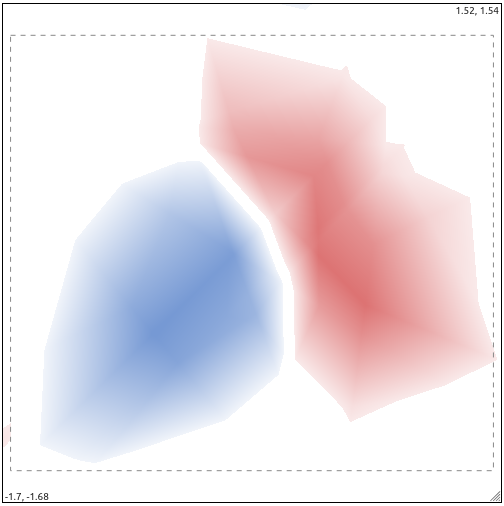
\includegraphics[width=0.24\linewidth]{Dissertation/images/ch4/algorithms_and_visualizations/model_output_linear.png}}
        \hfill
        \subcaptionbox{Дискретный режим}{
            \includegraphics[width=0.24\linewidth]{Dissertation/images/ch4/algorithms_and_visualizations/model_output_discrete.png}}
        \hfill
        \subcaptionbox{Дискретный режим на 10 уровней}{
            \includegraphics[width=0.24\linewidth]{Dissertation/images/ch4/algorithms_and_visualizations/model_output_discrete10.png}}
        \hfill
        \subcaptionbox{3D режим}{
            \includegraphics[width=0.24\linewidth]{Dissertation/images/ch4/algorithms_and_visualizations/model_output_3d.png}}
        \hfill
    }
    \caption{Визуализация выхода модели}
    \label{fig:vis_model_output}
\end{figure}

\begin{figure}[ht]
    \centerfloat{
        \hfill
        \subcaptionbox{Ячейки первого скрытого слоя}{%
            \includegraphics[width=0.3\linewidth]{Dissertation/images/ch4/algorithms_and_visualizations/cells1.png}}
        \hfill
        \subcaptionbox{Ячейки второго скрытого слоя}{%
            \includegraphics[width=0.3\linewidth]{Dissertation/images/ch4/algorithms_and_visualizations/cells2.png}}
        \hfill
        \subcaptionbox{Ячейки выходного слоя}{%
            \includegraphics[width=0.3\linewidth]{Dissertation/images/ch4/algorithms_and_visualizations/cells3.png}}
        \hfill
    }
    \caption{Визуализация иерархического разбиения на ячейки}
    \label{fig:vis_cells}
\end{figure}

\begin{figure}[ht]
    \centerfloat{
        \hfill
        \subcaptionbox{Метрики\label{fig:vis_metrics_hist_metrics}}{%
            \includegraphics[width=0.4\linewidth]{Dissertation/images/ch4/algorithms_and_visualizations/metrics.png}}
        \hfill
        \subcaptionbox{Гистограммы выхода модели\label{fig:vis_metrics_hist_hist}}{%
            \includegraphics[width=0.59\linewidth]{Dissertation/images/ch4/algorithms_and_visualizations/histograms.png}}
        \hfill
    }
    \caption{Визуализация метрик и гистограмм распределения выхода персептрона на обучающих данных}
    \label{fig:vis_metrics_hist}
\end{figure}

Для генерации графических представлений используются встроенные средства Canvas API и SVG с ручной реализацией всех визуальных компонентов. Визуализация обновляется в реальном времени по мере обучения модели. Для трёхмерного отображения выхода модели используется единственная внешняя зависимость Plotly.js~\cite{sievert2021package}.

%%%%%%%%%%%%%%%%%%%%%%%%%%%%%%%%%%%%%%%%%%%%%%%%%%%%%%%%%%%%%%%%%%%%%%%%%%%%%%%%%%%%%%%%%%%%%%%%%%%%%%%%%%%%%%%
\subsection{Анализ отказов от классификации}
Оценка надёжности классификации осуществляется с использованием порогового механизма, основанного на параметре доверия \(\beta\). При выходном значении, не превышающем порог \(\beta\), модель отказывается от классификации, помечая объект как нераспознанный. Это позволяет существенно повысить доверие к решениям, принятым моделью, особенно в задачах с высокой ценой ошибки.

Реализована визуализация распределения отказов: гистограммы выходных значений и графики зависимости доли отказов и точности от выбранного порога.

%%%%%%%%%%%%%%%%%%%%%%%%%%%%%%%%%%%%%%%%%%%%%%%%%%%%%%%%%%%%%%%%%%%%%%%%%%%%%%%%%%%%%%%%%%%%%%%%%%%%%%%%%%%%%%%
\subsection{Генерация и модификация данных}
Система включает инструменты генерации заранее подготовленных наборов данных для обучения и тестирования (рисунок~\cref{fig:vis_data}). Пользователь может настраивать следующие параметры:

\begin{itemize}
    \item Размер обучающей и тестовой выборки и их соотношение.
    \item Пропорции (баланс) классов.
    \item Доля ошибочно размеченных наблюдений.
    \item Нормализация, стандартизация и масштабирование признаков.
\end{itemize}

\begin{figure}[ht]
    \centerfloat{
        \hfill
        \subcaptionbox{набор данных ``Спираль``}{%
            \includegraphics[width=0.24\linewidth]{Dissertation/images/ch4/algorithms_and_visualizations/data_spiral.png}}
        \hfill
        \subcaptionbox{набор данных ``Окружность``}{%
            \includegraphics[width=0.24\linewidth]{Dissertation/images/ch4/algorithms_and_visualizations/data_circle.png}}
        \hfill
        \subcaptionbox{набор данных ``Moons``}{%
            \includegraphics[width=0.24\linewidth]{Dissertation/images/ch4/algorithms_and_visualizations/data_moons.png}}
        \hfill
        \subcaptionbox{набор данных ``Гауссианы``}{%
            \includegraphics[width=0.24\linewidth]{Dissertation/images/ch4/algorithms_and_visualizations/data_gaussians.png}}
        \hfill
    }
    \caption{Примеры наборов данных, доступных в интеллектуальной системе}
    \label{fig:vis_data}
\end{figure}

\section{Структура и функциональные компоненты пользовательского интерфейса}

Разработанная интеллектуальная система машинного обучения имеет модульную архитектуру пользовательского интерфейса, организованного в виде тематических вкладок. Такой подход позволяет изолировать различные этапы исследования и обеспечить пользователю интуитивно понятную навигацию между функциональными блоками. Вкладки интерфейса включают: ``Данные``, ``Обучение`` и ``Эксперименты``. Каждая из вкладок реализует отдельный аспект взаимодействия с системой.

\paragraph{Вкладка ``Данные``.} На данной вкладке пользователь может создавать обучающие и тестовые выборки, управляя их параметрами с помощью наглядных графических контроллеров, а также загружать данные из csv файлов. В числе доступных настроек:
\begin{itemize}
    \item выбор числа объектов и размерности признаков;
    \item задание доли тестовых данных;
    \item задание доли объектов каждого класса;
    \item включение ошибок разметки;
    \item выполнение нормализации и стандартизации признаков.
\end{itemize}

Созданные или загруженные данные визуализируются на двумерной плоскости с использованием цветовой кодировки классов.

\paragraph{Вкладка ``Обучение``.} Данный раздел интерфейса предназначен для настройки архитектуры модели, параметров её обучения и визуального отображения различных элементов. Пользователь может:
\begin{itemize}
    \item выбирать структуру многослойного персептрона (число слоёв, нейронов, функций активации);
    \item задавать параметры оптимизации (тип оптимизатора, скорость обучения, параметры регуляризации, функцию потерь);
    \item управлять отображение данных, сетки, ячеек и режимом выхода модели;
    \item запускать процесс обучения с возможностью пошагового анализа и прерывания.
\end{itemize}

Обучение сопровождается в реальном времени визуализацией различных характеристик: поверхности выходной функции модели, изменения функции ошибки, доли ошибок на обучающем и тестовом множествах, а также показателей отказа от классификации в зависимости от порога доверия.

\paragraph{Вкладка ``Эксперименты``.} Этот раздел агрегирует инструменты для проведения углублённого анализа результатов. В частности, доступны:
\begin{itemize}
    \item визуализация объясняющего двоичного дерева;
    \item создание синтетических данных на основе обученной модели;
    \item обучение модели на данных с искусственно внесёнными пропусками.
\end{itemize}

Для каждой из опций предусмотрено графическое отображение и интуитивно понятная система управления с наглядными пояснениями каждого шага и полученных результатов. Это делает модуль эффективным инструментом для анализа моделей в условиях ограниченного количества данных, дисбаланса классов и наличия пропусков.

\section{Алгоритмы визуализации}

Графическая составляющая интеллектуальной системы реализована с использованием низкоуровневых возможностей браузера, таких как SVG и HTML5 Canvas API. Отказ от сторонних библиотек в пользу чистого JavaScript и CSS обусловлен требованиями к производительности, контролю над прорисовкой и необходимости точной синхронизации между визуальными компонентами.

Отрисовка данных, поверхности выхода модели, границ принятия решений, зон отказа от классификации, а также метрик качества осуществляется в режиме реального времени. Обновление изображений происходит по мере поступления новых данных или изменения параметров модели.

Основные принципы реализации визуализации включают:

\begin{itemize}
    \item использование Canvas API для эффективной отрисовки цветных карт выхода модели;
    \item применение SVG для отрисовки больших массивов точек, осей, подписей, интерактивных маркеров и других элементов управления;
    \item разделение визуальных компонентов на независимые модули, каждый из которых регистрирует себя как подписчик событий модели и наборов данных;
    \item организация обмена сообщениями между компонентами через реализацию событийной модели на базе шаблона EventEmitter;
    \item использование аппаратного ускорения браузера при отрисовке и обновлении графических элементов;
    \item минимизация количества полных перерисовок за счёт дифференциального обновления слоёв.
\end{itemize}

Особое внимание уделяется синхронности всех отображаемых компонентов и их согласованности с текущим состоянием модели. Каждый визуализируемый объект автоматически обновляется при изменении состояния, что позволяет пользователю в реальном времени отслеживать последствия своих действий.

\section{Примеры использования}

Интеллектуальная система машинного обучения была разработана с целью поддержки полного цикла исследования поведения нейросетевых моделей, включая этапы создания данных, обучения классификатора, анализа и интерпретации результатов. Ниже приведены ключевые сценарии использования системы, иллюстрирующие её функциональные возможности.

%%%%%%%%%%%%%%%%%%%%%%%%%%%%%%%%%%%%%%%%%%%%%%%%%%%%%%%%%%%%%%%%%%%%%%%%%%%%%%%%%%%%%%%%%%%%%%%%%%%%%%%%%%%%%%%
\subsection{Бинарная классификация}
Для проверки способности модели к нелинейной аппроксимации границ принятия решений решается задача классификации двух переплетённых спиралей (рисунок~\cref{fig:vis_binary_classification}). В системе предусмотрена генерация соответствующего набора данных и обучение модели с возможностью пошагового отображения изменения решения по мере выполнения эпохи градиентного спуска. Интеллектуальная система машинного обучения позволяет наблюдать как локальные ошибки, так и итоговую зону классификации, что особенно полезно при выборе архитектуры сети и прочих гиперпараметров.

\begin{figure}[ht]
    \centerfloat{
        \includegraphics[width=0.9\linewidth]{Dissertation/images/ch4/usage/binary_classification.png}
    }
    \caption{Пример выполнения бинарной классификации}
    \label{fig:vis_binary_classification}
\end{figure}

%%%%%%%%%%%%%%%%%%%%%%%%%%%%%%%%%%%%%%%%%%%%%%%%%%%%%%%%%%%%%%%%%%%%%%%%%%%%%%%%%%%%%%%%%%%%%%%%%%%%%%%%%%%%%%%
\subsection{Унарная классификация}
Режим унарной классификации допускает обучение модели только по положительным примерам, дополненным фоновыми объектами (рисунок~\cref{fig:vis_unary_classification}). В качестве примера используется одна из спиралей из предыдущего эксперимента. Пользователь может задать уровень порога \(\beta\), визуализировать полученную область принятия положительного класса, а также проследить, каким образом меняется зона отказа при варьировании параметров. Данный сценарий позволяет исследовать свойство доверия, характерное для унарных моделей.

\begin{figure}[ht]
    \centerfloat{
        \includegraphics[width=0.9\linewidth]{Dissertation/images/ch4/usage/unary_classification.png}
    }
    \caption{Пример выполнения унарной классификации}
    \label{fig:vis_unary_classification}
\end{figure}

%%%%%%%%%%%%%%%%%%%%%%%%%%%%%%%%%%%%%%%%%%%%%%%%%%%%%%%%%%%%%%%%%%%%%%%%%%%%%%%%%%%%%%%%%%%%%%%%%%%%%%%%%%%%%%%
\subsection{Создание синтетических данных}
Одной из оригинальных функций системы является реализация метода синтетической генерации данных на основе репродукции, предложенного в рамках диссертационного исследования. Данный метод позволяет строить приближённую аппроксимацию распределения положительного класса в пространстве признаков, используя предварительно обученную унарную модель (рисунок~\cref{fig:vis_synthetic_data}).

\begin{figure}[ht]
    \centerfloat{
        \includegraphics[width=0.9\linewidth]{Dissertation/images/ch4/usage/synthetic_data.png}
    }
    \caption{Пример построения синтетических данных}
    \label{fig:vis_synthetic_data}
\end{figure}

Пользователь может интерактивно варьировать пороговое значение, наблюдать за плотностью отобранных объектов, а также визуализировать геометрию полученного множества. Данная возможность особенно важна при построении новых обучающих выборок, моделировании редких классов и оценке обобщающей способности модели на слабо покрытых областях признакового пространства.

%%%%%%%%%%%%%%%%%%%%%%%%%%%%%%%%%%%%%%%%%%%%%%%%%%%%%%%%%%%%%%%%%%%%%%%%%%%%%%%%%%%%%%%%%%%%%%%%%%%%%%%%%%%%%%%
\subsection{Построение объясняющего дерева решений}
Одним из компонентов системы является модуль построения объясняющего дерева решений, предназначенного для геометрического описания поведения и интерпретации решения обученного персептрона (рисунок~\cref{fig:vis_extree}). Пользователь может выбрать интересующую ячейку и подробно изучить как её содержимое, так и геометрию пространства. Это позволяет проводить интерпретацию решения в выбранной области и служит средством повышения доверия к результатам классификации.

\begin{figure}[ht]
    \centerfloat{
        \includegraphics[width=0.9\linewidth]{Dissertation/images/ch4/usage/extree.png}
    }
    \caption{Пример работы с объясняющим деревом}
    \label{fig:vis_extree}
\end{figure}

\section{Роль интеллектуальной системы в исследовании}

Разработанная интеллектуальная система машинного обучения стала ключевым инструментом, обеспечивающим как реализацию предложенных в диссертации методов, так и всестороннюю экспериментальную проверку их свойств. Её архитектура ориентирована на гибкую настройку параметров моделей, визуальный контроль над процессом обучения, а также глубокий анализ поведения классификатора в условиях, приближённых к реальным сценариям применения.

Интеллектуальная система позволила оперативно проверять влияние архитектурных параметров нейронной сети на её аппроксимационные способности. Использование многослойного персептрона в качестве доверенного аппроксиматора вероятности принадлежности объекта к классу потребовало детальной настройки числа слоёв, функции активации и порога отказа \(\beta\). Все эти параметры доступны для интерактивного изменения в ходе экспериментов.

Интеллектуальная система была использована для воспроизведения поведения модели на данных с перекрытием классов и в условиях неопределённости. Визуализация границ принятия решений и отказа от классификации показала, как повышение порога \(\beta\) повышает надёжность предсказаний за счёт исключения сомнительных точек. Такие наблюдения трудно формализовать численно, но они критичны для практической интерпретации поведения модели.

Кроме того, интеллектуальная система оказалась удобной платформой для отладки и тестирования предложенной модификации классификатора в условиях ограниченного объёма данных и несбалансированности классов. Возможность быстрой генерации обучающих выборок и отображения результатов классификации в реальном времени позволила провести сотни запусков, лежащих в основе статистической оценки качества.

Таким образом, интеллектуальная система машинного обучения выполнила не только вспомогательную, но и методологически значимую роль, обеспечив воспроизводимость, наглядность и полноту исследования. Её использование позволило обосновать теоретические положения диссертации эмпирически, за счёт детального анализа поведения моделей на управляемых синтетических данных.

           % Глава 4

\chapter*{Заключение}                       % Заголовок
\addcontentsline{toc}{chapter}{Заключение}  % Добавляем его в оглавление

%% Согласно ГОСТ Р 7.0.11-2011:
%% 5.3.3 В заключении диссертации излагают итоги выполненного исследования, рекомендации, перспективы дальнейшей разработки темы.
%% 9.2.3 В заключении автореферата диссертации излагают итоги данного исследования, рекомендации и перспективы дальнейшей разработки темы.
%% Поэтому имеет смысл сделать эту часть общей и загрузить из одного файла в автореферат и в диссертацию:

Основные результаты работы заключаются в следующем.
%% Согласно ГОСТ Р 7.0.11-2011:
%% 5.3.3 В заключении диссертации излагают итоги выполненного исследования, рекомендации, перспективы дальнейшей разработки темы.
%% 9.2.3 В заключении автореферата диссертации излагают итоги данного исследования, рекомендации и перспективы дальнейшей разработки темы.

\begin{enumerate}
    \item Разработан и реализован метод построения классификатора, обеспечивающего состоятельную аппроксимацию апостериорных вероятностей при дисбалансе классов и некомплектности данных за счёт использования модифицированного байесовского классификатора на основе многослойного персептрона.
    \item Разработаны методы генерации синтетических табличных данных и обработки некомплектных табличных данных на основе предложенного метода построения классификатора.
    \item Проведено экспериментальное исследование разработанных методов на модельных и прикладных данных для оценки устойчивости классификатора к дисбалансу классов, неполноте данных и корректности обработки объектов вне носителя обучающего распределения.
    \item Разработана интеллектуальная система машинного обучения, реализующая предложенные методы и обеспечивающая решение задач классификации табличных данных в условиях дисбаланса классов, некомплектности данных и высокой неопределённости вне носителя распределения.
\end{enumerate}


Полученные результаты относятся к направлениям исследований 4, 7, 8 и 9 паспорта специальности 2.3.5.
      % Заключение
\printnomenclature[3.5cm] % Значение ширины столбца с обозначениями стоит подбирать вручную
        % Список сокращений и условных обозначений
\chapter*{Словарь терминов}             % Заголовок
\addcontentsline{toc}{chapter}{Словарь терминов}  % Добавляем его в оглавление

\textbf{Классификация} -- задача машинного обучения, в которой требуется отнести объект к одному из заранее определённых классов.

\textbf{Унарная классификация} -- подход, при котором обучение производится только на объектах одного (целевого) класса, а остальные данные считаются фоновыми или неизвестными.

\textbf{Отказ от классификации} -- механизм, позволяющий модели не принимать решение о принадлежности к какому-либо классу при низком уровне уверенности.

\textbf{Порог доверия \(\beta\)} -- значение, определяющее минимальный уровень уверенности модели, при котором принимается решение о классификации объекта.

\textbf{Многослойный персептрон} -- класс искусственных нейронных сетей, состоящий из нескольких слоёв нейронов, каждый из которых связан с предыдущим полносвязным образом. Используется для аппроксимации сложных функций.

\textbf{Полносвязный слой} -- слой нейронной сети, в котором каждый нейрон соединён со всеми выходами предыдущего слоя.

\textbf{Аппроксимация} -- приближённое представление функции, заданной неявно, с помощью некоторой модели, например нейросети или гистограммы.

\textbf{Градиентный спуск} -- метод оптимизации, основанный на итеративном обновлении параметров модели в направлении антиградиента функции потерь.

\textbf{Оптимизаторы градиентного спуска} -- алгоритмы, используемые для настройки параметров модели в процессе обучения.

\textbf{Синтетические данные} -- искусственно сгенерированные данные, используемые для проверки гипотез, обучения моделей и проведения контролируемых экспериментов при отсутствии достаточного количества реальных данных.

\textbf{Объясняющее дерево} -- структура, позволяющая в интерпретируемой форме представить поведение модели путём построения дерева решений на выходных значениях модели.

\textbf{Нормализация признаков} -- преобразование признаков, приводящее их к единому масштабу для повышения устойчивости и скорости обучения.
      % Словарь терминов
\clearpage                                  % В том числе гарантирует, что список литературы в оглавлении будет с правильным номером страницы
%\hypersetup{ urlcolor=black }               % Ссылки делаем чёрными
%\providecommand*{\BibDash}{}                % В стилях ugost2008 отключаем использование тире как разделителя
\urlstyle{rm}                               % ссылки URL обычным шрифтом
\ifdefmacro{\microtypesetup}{\microtypesetup{protrusion=false}}{} % не рекомендуется применять пакет микротипографики к автоматически генерируемому списку литературы
\insertbibliofull                           % Подключаем Bib-базы: все статьи единым списком
% Режим с подсписками
%\insertbiblioexternal                      % Подключаем Bib-базы: статьи, не являющиеся статьями автора по теме диссертации
% Для вывода выберите и расскомментируйте одно из двух
%\insertbiblioauthor                        % Подключаем Bib-базы: работы автора единым списком 
%\insertbiblioauthorgrouped                 % Подключаем Bib-базы: работы автора сгруппированные (ВАК, WoS, Scopus и т.д.)
\ifdefmacro{\microtypesetup}{\microtypesetup{protrusion=true}}{}
\urlstyle{tt}                               % возвращаем установки шрифта ссылок URL
%\hypersetup{ urlcolor={urlcolor} }          % Восстанавливаем цвет ссылок
      % Список литературы
\clearpage
\ifdefmacro{\microtypesetup}{\microtypesetup{protrusion=false}}{} % не рекомендуется применять пакет микротипографики к автоматически генерируемым спискам
\listoffigures  % Список изображений

%%% Список таблиц %%%
% (ГОСТ Р 7.0.11-2011, 5.3.10)
\clearpage
\listoftables   % Список таблиц
\ifdefmacro{\microtypesetup}{\microtypesetup{protrusion=true}}{}
\newpage           % Списки таблиц и изображений (иллюстративный материал)

\setcounter{totalchapter}{\value{chapter}} % Подсчёт количества глав

% Настройки для приложений
\appendix
% Оформление заголовков приложений ближе к ГОСТ:
\setlength{\midchapskip}{20pt}
\renewcommand*{\afterchapternum}{\par\nobreak\vskip \midchapskip}
\renewcommand\thechapter{\Asbuk{chapter}} % Чтобы приложения русскими буквами нумеровались

\chapter{Свидетельства о государственной регистрации программ и ЭВМ}\label{app:A}

\includepdf[pages=-]{Dissertation/images/registrations/rid1.pdf}
\includepdf[pages=-]{Dissertation/images/registrations/rid2.pdf}
\includepdf[pages=-]{Dissertation/images/registrations/rid3.pdf}
\includepdf[pages=-]{Dissertation/images/registrations/rid4.pdf}

\chapter{Доказательства теорем}\label{app:B}

\section{Доказательство \cref{theorem:modified_bayesian}}\label{app:B1}

Доказательство опубликовано в работе~\cite{lukyanov2024extrapolation} совместно с Лукьяновым К.С., Яськовым П.А., Коваленко А.П. и Турдаковым Д.Ю..

\textbf{ДОПИСАТЬ ДОКАЗАТЕЛЬСТВО}

% \clearpage
% \refstepcounter{chapter}
        % Приложения

\setcounter{totalappendix}{\value{chapter}} % Подсчёт количества приложений

\end{document}
